% Options for packages loaded elsewhere
\PassOptionsToPackage{unicode}{hyperref}
\PassOptionsToPackage{hyphens}{url}
\PassOptionsToPackage{dvipsnames,svgnames,x11names}{xcolor}
%
\documentclass[
  letterpaper,
  DIV=11,
  numbers=noendperiod]{scrreprt}

\usepackage{amsmath,amssymb}
\usepackage{iftex}
\ifPDFTeX
  \usepackage[T1]{fontenc}
  \usepackage[utf8]{inputenc}
  \usepackage{textcomp} % provide euro and other symbols
\else % if luatex or xetex
  \usepackage{unicode-math}
  \defaultfontfeatures{Scale=MatchLowercase}
  \defaultfontfeatures[\rmfamily]{Ligatures=TeX,Scale=1}
\fi
\usepackage{lmodern}
\ifPDFTeX\else  
    % xetex/luatex font selection
\fi
% Use upquote if available, for straight quotes in verbatim environments
\IfFileExists{upquote.sty}{\usepackage{upquote}}{}
\IfFileExists{microtype.sty}{% use microtype if available
  \usepackage[]{microtype}
  \UseMicrotypeSet[protrusion]{basicmath} % disable protrusion for tt fonts
}{}
\makeatletter
\@ifundefined{KOMAClassName}{% if non-KOMA class
  \IfFileExists{parskip.sty}{%
    \usepackage{parskip}
  }{% else
    \setlength{\parindent}{0pt}
    \setlength{\parskip}{6pt plus 2pt minus 1pt}}
}{% if KOMA class
  \KOMAoptions{parskip=half}}
\makeatother
\usepackage{xcolor}
\setlength{\emergencystretch}{3em} % prevent overfull lines
\setcounter{secnumdepth}{5}
% Make \paragraph and \subparagraph free-standing
\makeatletter
\ifx\paragraph\undefined\else
  \let\oldparagraph\paragraph
  \renewcommand{\paragraph}{
    \@ifstar
      \xxxParagraphStar
      \xxxParagraphNoStar
  }
  \newcommand{\xxxParagraphStar}[1]{\oldparagraph*{#1}\mbox{}}
  \newcommand{\xxxParagraphNoStar}[1]{\oldparagraph{#1}\mbox{}}
\fi
\ifx\subparagraph\undefined\else
  \let\oldsubparagraph\subparagraph
  \renewcommand{\subparagraph}{
    \@ifstar
      \xxxSubParagraphStar
      \xxxSubParagraphNoStar
  }
  \newcommand{\xxxSubParagraphStar}[1]{\oldsubparagraph*{#1}\mbox{}}
  \newcommand{\xxxSubParagraphNoStar}[1]{\oldsubparagraph{#1}\mbox{}}
\fi
\makeatother

\usepackage{color}
\usepackage{fancyvrb}
\newcommand{\VerbBar}{|}
\newcommand{\VERB}{\Verb[commandchars=\\\{\}]}
\DefineVerbatimEnvironment{Highlighting}{Verbatim}{commandchars=\\\{\}}
% Add ',fontsize=\small' for more characters per line
\usepackage{framed}
\definecolor{shadecolor}{RGB}{241,243,245}
\newenvironment{Shaded}{\begin{snugshade}}{\end{snugshade}}
\newcommand{\AlertTok}[1]{\textcolor[rgb]{0.68,0.00,0.00}{#1}}
\newcommand{\AnnotationTok}[1]{\textcolor[rgb]{0.37,0.37,0.37}{#1}}
\newcommand{\AttributeTok}[1]{\textcolor[rgb]{0.40,0.45,0.13}{#1}}
\newcommand{\BaseNTok}[1]{\textcolor[rgb]{0.68,0.00,0.00}{#1}}
\newcommand{\BuiltInTok}[1]{\textcolor[rgb]{0.00,0.23,0.31}{#1}}
\newcommand{\CharTok}[1]{\textcolor[rgb]{0.13,0.47,0.30}{#1}}
\newcommand{\CommentTok}[1]{\textcolor[rgb]{0.37,0.37,0.37}{#1}}
\newcommand{\CommentVarTok}[1]{\textcolor[rgb]{0.37,0.37,0.37}{\textit{#1}}}
\newcommand{\ConstantTok}[1]{\textcolor[rgb]{0.56,0.35,0.01}{#1}}
\newcommand{\ControlFlowTok}[1]{\textcolor[rgb]{0.00,0.23,0.31}{\textbf{#1}}}
\newcommand{\DataTypeTok}[1]{\textcolor[rgb]{0.68,0.00,0.00}{#1}}
\newcommand{\DecValTok}[1]{\textcolor[rgb]{0.68,0.00,0.00}{#1}}
\newcommand{\DocumentationTok}[1]{\textcolor[rgb]{0.37,0.37,0.37}{\textit{#1}}}
\newcommand{\ErrorTok}[1]{\textcolor[rgb]{0.68,0.00,0.00}{#1}}
\newcommand{\ExtensionTok}[1]{\textcolor[rgb]{0.00,0.23,0.31}{#1}}
\newcommand{\FloatTok}[1]{\textcolor[rgb]{0.68,0.00,0.00}{#1}}
\newcommand{\FunctionTok}[1]{\textcolor[rgb]{0.28,0.35,0.67}{#1}}
\newcommand{\ImportTok}[1]{\textcolor[rgb]{0.00,0.46,0.62}{#1}}
\newcommand{\InformationTok}[1]{\textcolor[rgb]{0.37,0.37,0.37}{#1}}
\newcommand{\KeywordTok}[1]{\textcolor[rgb]{0.00,0.23,0.31}{\textbf{#1}}}
\newcommand{\NormalTok}[1]{\textcolor[rgb]{0.00,0.23,0.31}{#1}}
\newcommand{\OperatorTok}[1]{\textcolor[rgb]{0.37,0.37,0.37}{#1}}
\newcommand{\OtherTok}[1]{\textcolor[rgb]{0.00,0.23,0.31}{#1}}
\newcommand{\PreprocessorTok}[1]{\textcolor[rgb]{0.68,0.00,0.00}{#1}}
\newcommand{\RegionMarkerTok}[1]{\textcolor[rgb]{0.00,0.23,0.31}{#1}}
\newcommand{\SpecialCharTok}[1]{\textcolor[rgb]{0.37,0.37,0.37}{#1}}
\newcommand{\SpecialStringTok}[1]{\textcolor[rgb]{0.13,0.47,0.30}{#1}}
\newcommand{\StringTok}[1]{\textcolor[rgb]{0.13,0.47,0.30}{#1}}
\newcommand{\VariableTok}[1]{\textcolor[rgb]{0.07,0.07,0.07}{#1}}
\newcommand{\VerbatimStringTok}[1]{\textcolor[rgb]{0.13,0.47,0.30}{#1}}
\newcommand{\WarningTok}[1]{\textcolor[rgb]{0.37,0.37,0.37}{\textit{#1}}}

\providecommand{\tightlist}{%
  \setlength{\itemsep}{0pt}\setlength{\parskip}{0pt}}\usepackage{longtable,booktabs,array}
\usepackage{multirow}
\usepackage{calc} % for calculating minipage widths
% Correct order of tables after \paragraph or \subparagraph
\usepackage{etoolbox}
\makeatletter
\patchcmd\longtable{\par}{\if@noskipsec\mbox{}\fi\par}{}{}
\makeatother
% Allow footnotes in longtable head/foot
\IfFileExists{footnotehyper.sty}{\usepackage{footnotehyper}}{\usepackage{footnote}}
\makesavenoteenv{longtable}
\usepackage{graphicx}
\makeatletter
\def\maxwidth{\ifdim\Gin@nat@width>\linewidth\linewidth\else\Gin@nat@width\fi}
\def\maxheight{\ifdim\Gin@nat@height>\textheight\textheight\else\Gin@nat@height\fi}
\makeatother
% Scale images if necessary, so that they will not overflow the page
% margins by default, and it is still possible to overwrite the defaults
% using explicit options in \includegraphics[width, height, ...]{}
\setkeys{Gin}{width=\maxwidth,height=\maxheight,keepaspectratio}
% Set default figure placement to htbp
\makeatletter
\def\fps@figure{htbp}
\makeatother

\KOMAoption{captions}{tableheading}
\makeatletter
\@ifpackageloaded{tcolorbox}{}{\usepackage[skins,breakable]{tcolorbox}}
\@ifpackageloaded{fontawesome5}{}{\usepackage{fontawesome5}}
\definecolor{quarto-callout-color}{HTML}{909090}
\definecolor{quarto-callout-note-color}{HTML}{0758E5}
\definecolor{quarto-callout-important-color}{HTML}{CC1914}
\definecolor{quarto-callout-warning-color}{HTML}{EB9113}
\definecolor{quarto-callout-tip-color}{HTML}{00A047}
\definecolor{quarto-callout-caution-color}{HTML}{FC5300}
\definecolor{quarto-callout-color-frame}{HTML}{acacac}
\definecolor{quarto-callout-note-color-frame}{HTML}{4582ec}
\definecolor{quarto-callout-important-color-frame}{HTML}{d9534f}
\definecolor{quarto-callout-warning-color-frame}{HTML}{f0ad4e}
\definecolor{quarto-callout-tip-color-frame}{HTML}{02b875}
\definecolor{quarto-callout-caution-color-frame}{HTML}{fd7e14}
\makeatother
\makeatletter
\@ifpackageloaded{bookmark}{}{\usepackage{bookmark}}
\makeatother
\makeatletter
\@ifpackageloaded{caption}{}{\usepackage{caption}}
\AtBeginDocument{%
\ifdefined\contentsname
  \renewcommand*\contentsname{Table of contents}
\else
  \newcommand\contentsname{Table of contents}
\fi
\ifdefined\listfigurename
  \renewcommand*\listfigurename{List of Figures}
\else
  \newcommand\listfigurename{List of Figures}
\fi
\ifdefined\listtablename
  \renewcommand*\listtablename{List of Tables}
\else
  \newcommand\listtablename{List of Tables}
\fi
\ifdefined\figurename
  \renewcommand*\figurename{Figure}
\else
  \newcommand\figurename{Figure}
\fi
\ifdefined\tablename
  \renewcommand*\tablename{Table}
\else
  \newcommand\tablename{Table}
\fi
}
\@ifpackageloaded{float}{}{\usepackage{float}}
\floatstyle{ruled}
\@ifundefined{c@chapter}{\newfloat{codelisting}{h}{lop}}{\newfloat{codelisting}{h}{lop}[chapter]}
\floatname{codelisting}{Listing}
\newcommand*\listoflistings{\listof{codelisting}{List of Listings}}
\makeatother
\makeatletter
\makeatother
\makeatletter
\@ifpackageloaded{caption}{}{\usepackage{caption}}
\@ifpackageloaded{subcaption}{}{\usepackage{subcaption}}
\makeatother

\ifLuaTeX
  \usepackage{selnolig}  % disable illegal ligatures
\fi
\usepackage{bookmark}

\IfFileExists{xurl.sty}{\usepackage{xurl}}{} % add URL line breaks if available
\urlstyle{same} % disable monospaced font for URLs
\hypersetup{
  pdftitle={Open Science: Wie sich die Wissenschaft öffnet},
  pdfauthor={Lukas Röseler},
  colorlinks=true,
  linkcolor={blue},
  filecolor={Maroon},
  citecolor={Blue},
  urlcolor={Blue},
  pdfcreator={LaTeX via pandoc}}


\title{Open Science: Wie sich die Wissenschaft öffnet}
\author{Lukas Röseler}
\date{}

\begin{document}
\maketitle

\renewcommand*\contentsname{Table of contents}
{
\hypersetup{linkcolor=}
\setcounter{tocdepth}{2}
\tableofcontents
}

\bookmarksetup{startatroot}

\chapter*{Willkommen}\label{willkommen}
\addcontentsline{toc}{chapter}{Willkommen}

\markboth{Willkommen}{Willkommen}

\begin{tcolorbox}[enhanced jigsaw, bottomrule=.15mm, toprule=.15mm, opacitybacktitle=0.6, breakable, colback=white, coltitle=black, bottomtitle=1mm, toptitle=1mm, titlerule=0mm, title=\textcolor{quarto-callout-caution-color}{\faFire}\hspace{0.5em}{Warnung}, rightrule=.15mm, arc=.35mm, opacityback=0, leftrule=.75mm, left=2mm, colbacktitle=quarto-callout-caution-color!10!white, colframe=quarto-callout-caution-color-frame]

Dieses Projekt befindet sich in Arbeit und ist aktuell noch unfertig!
Texte sind unvollständig oder fehlen, Quellenangaben und Abbildungen
sind vorläufig, und es wimmelt von Rechtschreibfelehrn\ldots{}

\end{tcolorbox}

Viele wissenschaftliche Disziplinen haben sich in den letzten Jahren
stark verändert. Neue Zeitschriften, Methoden, Initiativen,
Gesellschaften, Strukturen, und vieles mehr sind entstanden. Es ist die
Rede von einer Krise {[}@Mede.2020{]}, einer Revolution {[}@Nosek.{]}
oder einer Renaissance {[}@Nelson.2018.{]}. All diese Veränderungen
haben gemeinsam zu einem stärkeren Grad an Offenheit und Transparenz
geführt und das Wissenschaftssystem maßgeblich verändert.

In diesem Buch werden niedrigschwellig der Begriff der Offenheit, die
Ursprünge des Wandels, und die Open Science Bewegung erklärt. Es werden
Hintergründe des wissenschaftlichen Systems, neu entwickelte Methoden,
und Probleme amtierender Methoden erläutert. Dabei wird vorwiegend auf
Beispiele und Entwicklungen aus der Psychologie zurückgegriffen.

\section*{Literatur}\label{literatur}
\addcontentsline{toc}{section}{Literatur}

\markright{Literatur}

\bookmarksetup{startatroot}

\chapter{Über das Buch}\label{uxfcber-das-buch}

Wissenschaft wird zu einem Maßgeblichen Teil von Steuergeldern
finanziert. Das bedeutet, eine Gesellschaft fördert einzelne Personen,
um ein tieferes Verständnis von der Welt zu erlangen und im Gegenzug
Unterstützung bei der Lösung verschiedener Probleme zu erhalten. Dadurch
sind Wissenschaftler*innen der Gesellschaft in einem gewissen Maße
Rechenschaft schuldig. Dabei geht es nicht darum, dass jede
wissenschaftliche Erkenntnis notwendigerweise Früchte tragen muss, aber,
dass sie wissenschaftlichen Gütekriterien entspricht und zumindest für
andere Forschende nachvollziehbar und nachprüfbar ist. Inwiefern das in
verschiedenen Disziplinen der Fall ist und wie Personen sich dafür
einsetzen, diese Rechenschaft zu ermöglichen, möchte ich in diesem Buch
darlegen.

\begin{tcolorbox}[enhanced jigsaw, bottomrule=.15mm, toprule=.15mm, opacitybacktitle=0.6, breakable, colback=white, coltitle=black, bottomtitle=1mm, toptitle=1mm, titlerule=0mm, title=\textcolor{quarto-callout-note-color}{\faInfo}\hspace{0.5em}{Über mich}, rightrule=.15mm, arc=.35mm, opacityback=0, leftrule=.75mm, left=2mm, colbacktitle=quarto-callout-note-color!10!white, colframe=quarto-callout-note-color-frame]

Mein Name ist Lukas Röseler und ich bin Wissenschaftler. Ich habe in
Wernigerode Psychologie und Wirtschaftswissenschaften studiert, mich
darüber hinaus mit Philosophie und Wissenschaftstheorie beschäftigt, und
habe 2021 in Bamberg meinen Doktortitel in Psychologie erhalten. Seit
2023 bin ich Geschäftsführer des Münster Center for Open Science, darf
mich im Rahmen dessen mit transparenter und vertrauenswürdiger
Wissenschaft in zahlreichen Disziplinen auseinandersetzen. Dabei
betreibe ich Meta-Wissenschaft, also \emph{Wissenschaft über
Wissenschaft}.

Ich habe dieses Buch geschrieben, um das Thema \emph{Open Science}
anderen Wissenschaftler*innen, Studierenden, und allen anderen Personen
auf einem einfachen aber ausführlichen Niveau zu erklären. Ein großer
Aspekt von offener Wissenschaft ist nämlich, dass auch Personen von
außerhalb zumindest teilweise verstehen können, was dort vor sich geht.
Angesichts dieses Zieles ist das Buch kostenlos und online verfügbar.

\begin{figure}[H]

{\centering 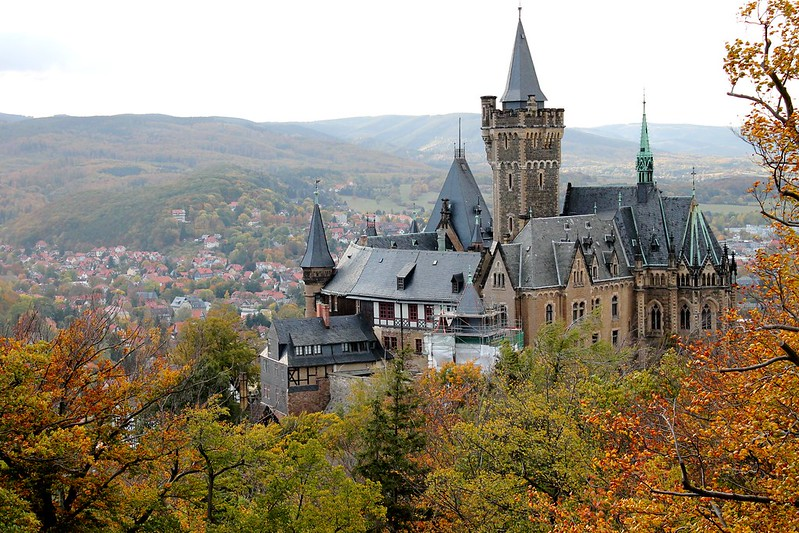
\includegraphics[width=6.25in,height=\textheight]{images/wernigerode.jpg}

}

\caption{Blick über Wernigerode}

\end{figure}%

\end{tcolorbox}

\part{Einleitung}

\section*{Einleitung}\label{einleitung-1}
\addcontentsline{toc}{section}{Einleitung}

\markright{Einleitung}

\part{Überschrift passend zum Beispiel}

-~~~~~~~~~ Beispiel, bei dem Psychologische Wissenschaft wichtig ist

-~~~~~~~~~ Befunde aus der Wissenschaft zitieren

-~~~~~~~~~ Diese Befunde sind eventuell falsch

-~~~~~~~~~ Wie finden wir heraus, ob sie falsch sind?

-~~~~~~~~~ Wie stark können wir uns darauf verlassen?

-~~~~~~~~~ Wie stellen wir sicher, dass wir uns stärker auf Wissenschaft
verlassen können?

\hyperref[_ftnref2]{{[}2{]}} Durch die Ungewissheit über genaue Ursachen
von geringen Replikationsraten wird teilweise auch eher zu dem Begriff
„Vertrauenskrise'' geraten (z.B. Feest, 2023).

~\hyperref[_msoanchor_1]{{[}LR1{]}}hier noch Wissenschaftsskepsis
erwähnen: \url{https://osf.io/preprints/psyarxiv/7u4fg} ~

~\hyperref[_msoanchor_2]{{[}LR2{]}}OS Taxonomie:
\url{https://periodicos.ufsc.br/index.php/eb/article/view/91712}

Bild

\url{https://zenodo.org/records/7940641}

~\hyperref[_msoanchor_3]{{[}LR3{]}}\url{https://www.researchgate.net/publication/374381552_What_is_the_Replication_Crisis_a_Crisis_of}

~\hyperref[_msoanchor_4]{{[}LR4{]}}hier Bild vom Spektrum und der
Verortung dieses Buches hintun; evtl. Umfrageergebnisse von
Wissenschaftler*innen dazutun und zitieren, da gibt es was

~\hyperref[_msoanchor_5]{{[}LR5{]}}Als Infobox

\chapter{Was ist Open Science?}\label{was-ist-open-science}

In der Wissenschaft dreht es sich oft um Details: Was genau passierte in
der Studie? Welche Bilder sahen Versuchspersonen auf was für einem
Bildschirm? Was war die Bildwiederholungsrate des Bildschirmes, und
waren die Farben dabei mittels Spektralphotometer kalibriert?
Wissenschaftliche Untersuchungen und ihre Befunde werden heutzutage in
Zeitschriftenartikeln beschrieben. Es kommt nicht selten vor, dass darin
eines der oben aufgeführten Details fehlt, in den Zusatzmaterialien
nicht auffindbar ist, oder die Autor*innen nicht gefragt werden können,
weil ihre E-Mail-Adresse nicht mehr aktuell ist. Wenn nun aber der
Befund von genauso einem Detail abhängt, werden zukünftige Forschende
Probleme haben, ihn zum Vorschein zu bringen. Auf dieser konkreten Ebene
bedeutet Open Science die Möglichkeit für jede Person, im Rahmen von
ethischen und legalen Einschränkungen (z.B. Anonymität), detaillierte
Einsicht in den gesamten wissenschaftlichen Prozess der
Erkenntnisgewinnung zu erhalten. Es sollte also genau beschrieben
werden, wie die Untersuchung ablief, welche Materialien dafür verwendet
werden, welche Daten daraus resultierten, wie diese weiterverarbeitet
und ausgewertet wurden, und schließlich, was daraus zu lernen ist.

Auf einer abstrakten Ebene meint Open Science einen höheren Grad an
Offenheit und Transparenz in allen Facetten der Wissenschaft. Dazu
gehören wie beschrieben Studienmaterialien (z.B. Fragebögen, Bilder,
oder Videos), der wissenschaftliche Bericht, oder der Diskurs im Rahmen
der Begutachtung wissenschaftlicher Berichte durch ihre Kolleg*innen
(Peer-Review). Aber auch auf der systemischen Ebene kann der Grad an
Transparenz steigen: Beispielsweise gibt es Listen mit Zeitschriften
(\url{https://doaj.org}) oder Listen mit Professuren in einem bestimmten
Wissenschaftsbereich (z.B. für die
\href{https://docs.google.com/spreadsheets/d/1XwO4n88zkdH1bDGpW6Uz8f4sH24P5FG0ihUp7i0Y-gY/edit\#gid=1684024252}{Persönlichkeitspsychologie
in Deutschland}). Schließlich kann mit Offenheit auch die Durchführung
einer Konferenz im „hybriden Format'', also an einem bestimmten Ort aber
mit der Möglichkeit zur Online-Teilnahme angeboten werden, um Personen,
die nicht Anreisen (können) nicht auszuschließen, ihnen gegenüber also
\emph{offen} zu sein.

Insgesamt wird Open Science als Lösung für zahlreiche aktuelle, meist
zusammenhängende Probleme verstanden, allen vorweg das Problem, dass
sich ungefähr 50\% aller wissenschaftlichen Studien in der Psychologie
nicht replizieren lassen {[}@OpenScienceCollaboration.2015{]}. Fecher
und Friesike ({[}@fecher2014open{]}, S. 19) reden von fünf „schools of
thought'', also Denkkollektiven, die verschiedene Ziele verfolgen:
Infrastruktur (z.B. Plattformen zum Speichern oder Veröffentlichen von
Forschungsmaterialien), Öffentlichkeit und Involvierung der Gesellschaft
in den wissenschaftlichen Prozess (z.B. Citizen Science), Messbarkeit
wissenschaftlichen Erfolgs (z.B. Alternativen zum Impact Factor),
Demokratie (z.B. Zugang zum Wissen), und Pragmatismus (z.B. höhere
Effizienz von Wissenschaften durch öffentliche Forschungsdaten). Eine
Übersicht über unsortierte Facetten von Open Science ist unten
abgebildet. Genaue Schätzungen sind schwierig, grob lässt sich dennoch
sagen: Sucht man sich eine zufällige sozialwissenschaftliche Studie aus
einer Fachzeitschrift aus, führt sie nach wissenschaftlichem
Goldstandard erneut aus, und prüft die dort getestete Hypothese ein
weiteres Mal, dann ist die Wahrscheinlichkeit, zum selben Ergebnis zu
kommen, so hoch, wie bei einem Münzwurf ``Zahl'' (vs.~Kopf) zu erhalten.
Damit teilweise verbundene Probleme sind Betrug bei wissenschaftlichen
Publikationen {[}@Gopalakrishna.2021{]}, oder psychische Probleme bei
Jungwissenschaftler*innen {[}@Satinsky.2021{]}.

\begin{figure}[H]

{\centering 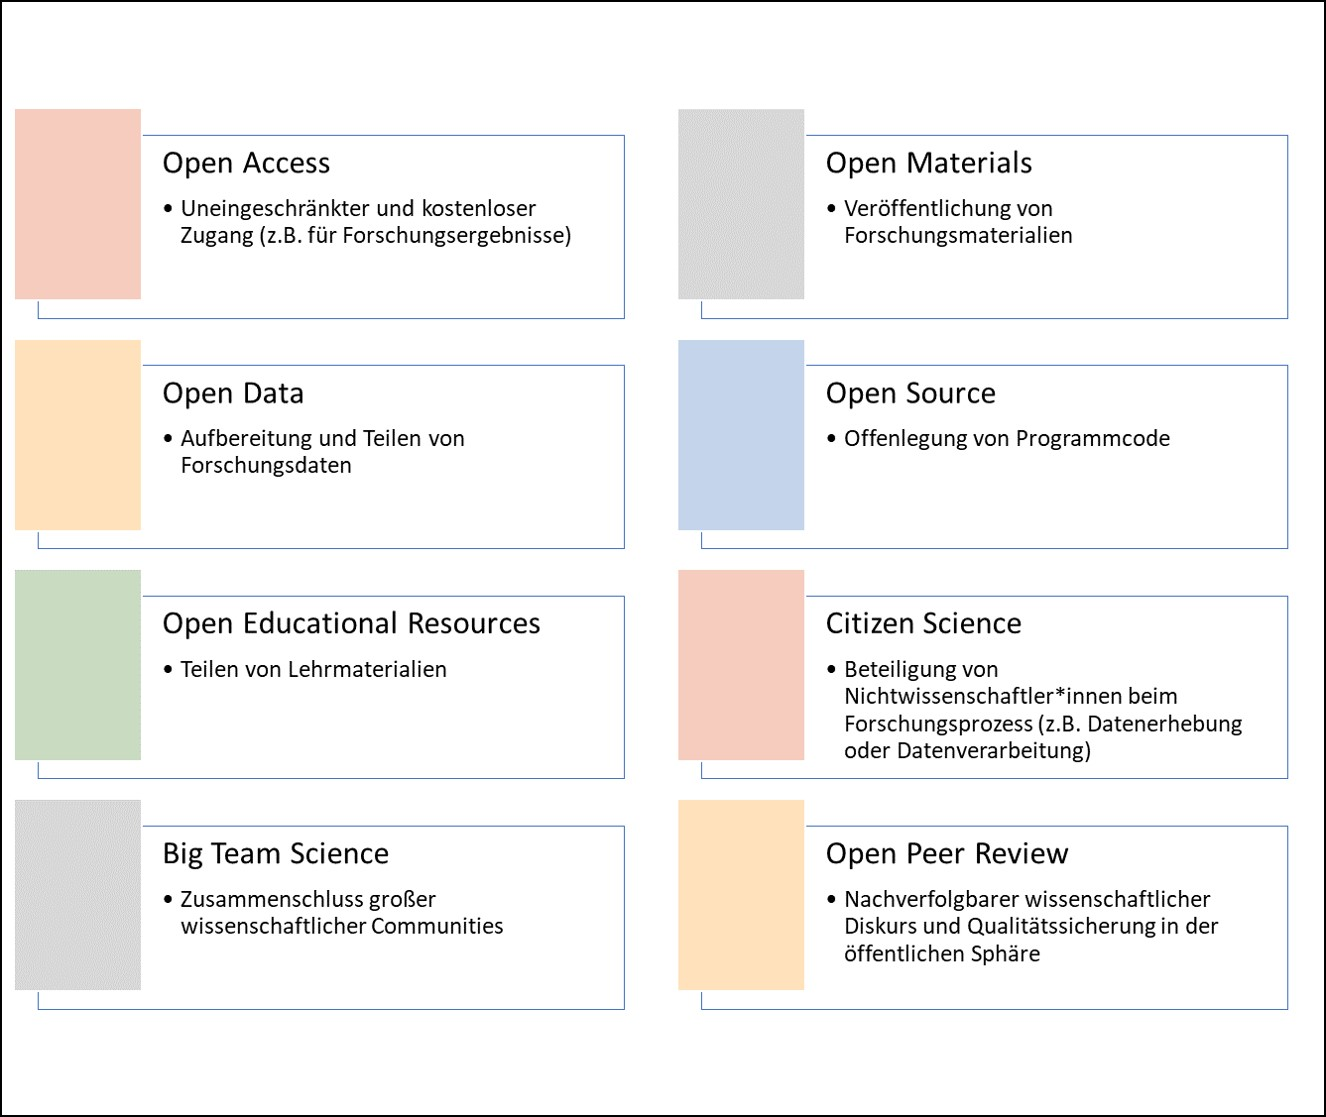
\includegraphics{images/facetten.jpg}

}

\caption{Facetten von Open Science}

\end{figure}%

\chapter{Wie ist mit Open Science
umzugehen?}\label{wie-ist-mit-open-science-umzugehen}

\textbf{Wie ist mit Open Science umzugehen?}

Das Thema Open Science und Replikationskrise beziehungsweise
Vertrauenskrise ist aus mehreren Gründen schwer kommunizierbar: Zuerst
einmal ist es harte Kritik an der Wissenschaft und dem
Wissenschaftssystem, die dazu missbraucht werden kann, wissenschaftliche
Befunde kleinzureden und das Vertrauen in Wissenschaft insgesamt
gefährdet. Mithilfe der hier präsentierten Argumente und Befunde lassen
sich zum Beispiel auf Wissenschaft beruhende politische oder
individuelle Entscheidungen kritisieren. Dagegen sei gesagt: Weitaus
nicht alle wissenschaftlichen Befunde sind ``falsch'' oder nicht
replizierbar. Bei vielen Punkten herrscht immer noch ein großer Konsens.

Auf der anderen Seite gehen die hier diskutierten Probleme über das
hinaus, was ganz natürlich in fast jedem wissenschaftlichen Zweig
wiederfindet. Denn je genauer man hinschaut, desto wahrscheinlicher ist
es, dass ein wissenschaftlicher Befund relativierbar ist. Widersprüche
oder Konflikte lassen sich überall finden, treten natürlicherweise auf,
und werden von Wissenschaftler*innen ins Visier genommen. Jede*r
Forschende kann berichten: Bei genauerem Hinschauen bleibt nichts
schwarz oder weiß, sondern zerfließt in viele Grautöne. Bei den im
Folgenden behandelten Replikationsfehlschlägen handelt es sich um mehr
als die wissenschaftsinhärente Ungewissheit: Sie gefährden gesamte
Wissenschaftsstränge.

Bevor wir in die Details fortschreiben, ist es außerdem wichtig
festzuhalten, dass aktuell (Herbst, 2023) die meisten der in diesem Buch
besprochenen Probleme noch nicht oder erst teilweise gelöst wurden und
auf wöchentlicher Basis heiß diskutiert werden. Nach einem Jahrzehnt der
Open Science Bewegungen ist ein Punkt erreicht, an dem die meisten
Wissenschaftler*innen ein Bewusstsein über das Problem haben. Einige
sind mit Lösungsansätzen vertraut, doch haben sich diese weder komplett
durchgesetzt, noch ist klar, welche Probleme überhaupt bereits gelöst
worden sind.

Ich verstehe Open Science als eine große Trigger-Warnung, die vor die
Sozialwissenschaften vorgeschaltet sein sollte und lautet: Achtung, wir
haben hier gerade sehr große Probleme. Es ist gut möglich, dass die
Hälfte von allem, was wir zu wissen glauben, schlichtweg falsch ist.
Meinungen über die Open Science Bewegung sind aber keineswegs homogen:
Es lässt sich hier ein Spektrum spannen zwischen ``Sollen wir wirklich
die nächsten 20 Jahre damit verbringen, herauszufinden, welche
Erkenntnisse der letzten 100 Jahre korrekt sind? Fangen wir doch einfach
nochmal bei Null an.'' und ``Eigentlich ist das ganz normal, ich sehe
keinen Grund, hier von einer `Krise' zu sprechen''.

\begin{figure}[H]

{\centering 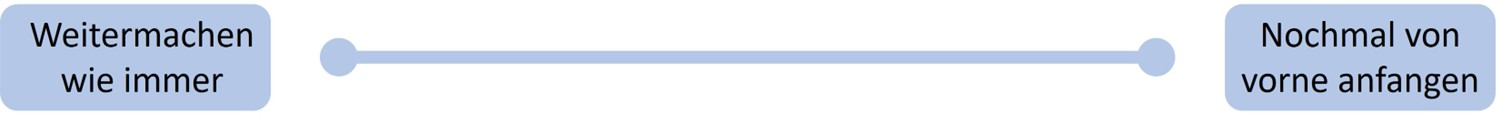
\includegraphics{images/spektrumreaktionen.jpg}

}

\caption{Spektrum der Reaktionen auf die Replikationskrise}

\end{figure}%

Besonders groß ist das Problem bei Lehrbüchern: Stellen Sie sich vor,
sie haben ein Buch über einen Teil der Psychologie (Aushängeschild ist
hier oft die Sozialpsychologie) verfasst, das auf Jahrzehnten an
Forschung besteht, hunderten Veröffentlichungen, und tausenden Studien.
Hier hilft es kaum, das Buch komplett zu ignorieren. Praktikabel, alle
Studien selbst zu replizieren, ist es allerdings auch nicht. Klar ist
den meisten Wissenschaftler*innen hierbei: So wie es bisher gelaufen
ist, kann es nicht weitergehen. Eine fünfzig prozentige Garantie für
wissenschaftliche Erkenntnisse sollte nicht der Anspruch von etwas sein,
das sich Wissenschaft nennt. Von vorne müssen wir aber auch nicht
starten.

\part{Die Geschichte der Open Science Bewegung}

\section*{Geschichte}\label{geschichte}
\addcontentsline{toc}{section}{Geschichte}

\markright{Geschichte}

Im Rahmen dieses Buches wird die Open Science Bewegung also als eine
Reaktion auf identifizierte Probleme und damit als
Selbstkorrektur-Prozess der Wissenschaft verstanden. In im Zentrum steht
ein mangelndes Vertrauen in Befunde, die in wissenschaftlichen
Fachzeitschriften veröffentlicht wurden. Einige Probleme sind schon seit
Jahrzehnten in ähnlicher Form bekannt. Bis sie allerdings öffentlich
diskutiert wurden und Lösungsvorschläge erarbeiteten, benötigte es
einschneidende Ereignisse. Aufgrund von Problemen, vergangene und für
sicher geglaubte Ergebnisse nicht \emph{replizieren} zu können (also bei
wiederholten Untersuchungen zum selben Ergebnis zu kommen) ist häufig
die Sprache von einer \emph{Replikationskrise}. Durch die Ungewissheit
über genaue Ursachen von geringen Replikationsraten wird teilweise auch
eher zu dem Begriff „Vertrauenskrise'' geraten {[}@Feest.c{]}.

\section*{Literatur}\label{literatur-1}
\addcontentsline{toc}{section}{Literatur}

\markright{Literatur}

\chapter{Anfänge einer Revolution}\label{anfuxe4nge-einer-revolution}

Um das Jahr 2010 herum häuften sich in der Psychologie Ereignisse, die
für sich genommen als Einzelfälle abgetan werden konnten, gemeinsam aber
ein negatives Bild der Wissenschaft zeichneten.

\subsection{Stapel-Affäre}\label{stapel-affuxe4re}

Durch einen Zufall entdeckten Nachwuchswissenschaftler im Jahr 2011,
dass die Daten einer Studie ihres Kollegen, Diederik Stapel, von
niemandem jemals erhoben wurden. Sie waren ausgedacht, bzw. fabriziert.
Stand Juli 2024 wurden 58 von Stapels Fachartikel identifiziert und
zurückgezogen, deren Daten fabriziert oder geschönt wurden.\footnote{Mittels
  der Retraction Database lassen sich nach Thema, Autor*in, Zeitschrift,
  usw. zurückgezogene Artikel durchsuchen:
  http://retractiondatabase.org/} Wissenschaftliche Institutionen wie
der Begutachtungsprozess von Artikeln durch Fachkolleg*inen, deren Zweck
die Qualitätssicherung war, hatten versagt. Seit dem Vorfall sind einige
weitere Fälle bekannt geworden, teilweise durch erneute Analyse von
Daten der jeweiligen Studien {[}@o2021honesty{]} und oft durch
Whistleblower, also durch Personen, die zu ihrem Schutz anonym bleiben
wollen. Umfragen in den Niederlanden unter Forschenden haben ergeben,
dass Fälschung oder Schönigung von Daten von bis zu 10\% aller Personen
durchgeführt wird {[}@Gopalakrishna.2021b{]}. Dabei ist zu beachten,
dass Studien durch gefälschte Daten besonders innovativ, überraschend,
oder klar werden - Eigenschaften, die die Veröffentlichung in einer
Fachzeitschrift wahrscheinlicher machen.

\subsection{Bem: Die Zukunft
erfühlen}\label{bem-die-zukunft-erfuxfchlen}

Kurze Zeit später veröffentliche Daryl Bem, bekannt durch grundlegende
psychologisch-philosophische Theorien wie der Self-Perception-Theory
{[}@Bem.1967{]}, den Befund, dass Personen die Zukunft vorhersagen
können {[}@Bem.2011{]}. Genauer gesagt, können manche Personen unter
bestimmten Dingen, die Zukunft vorhersagen. In 8 Studien fand die
Forschendengruppe, dass Personen Vorhersagen über erotische Bilder
machen konnten. Die Ergebnisse wurden in der hoch angesehenen
Fachzeitschrift \emph{Journal of Personality and Social Psychology}
veröffentlicht. Vielen Psycholog*innen war sofort klar: Entweder,
Grundlegende Annahmen ihres Weltbildes waren falsch (``Personen können
nicht die Zukunft vorhersagen'') oder es stimmte etwas mit den
Ergebnissen nicht. Mehrere Forschende versuchten sich daran, zu
erklären, wie es zu den Ergebnissen kam. Analysen mit alternativen
statistischen Methoden führten zur selben Schlussfolgerung
{[}@Wagenmakers.2011{]}, Replikationen durch unabhängige Forschende
schlugen jedoch fehl {[}@robinson2011not, @muhmenthaler2022future,
@roe2012feeling{]}.

\subsection{\texorpdfstring{Bargh: Beeinflussen durch
\emph{Priming}}{Bargh: Beeinflussen durch Priming}}\label{bargh-beeinflussen-durch-priming}

Seine Studien wurden im Marketing gefeiert und als
Neurowissenschaftliche Erkenntnisse verkauft: Wer ein heißes Getränk (im
Vergleich zu einem kalten) trinkt, schätzt andere Personen als
``wärmer'' (großzügig, rücksichtsvoll) ein
{[}@williams2008experiencing{]}. Wer Anagramme löst, die etwas mit hohem
Alter zu tun haben (z.B. PFLEGEHEIM, GRAU, oder zum selbst probieren
GHOSTECK), geht danach in langsamerem Tempo
{[}@bargh1996automaticity{]}. Viele dieser Studien wurden repliziert:
Forschenden fiel in der Anagramme-Studie auf, dass Bargh und
Kolleg*innen die Zeit mit Stoppuhren gemessen hatten und dabei wussten,
welche Person die ``Alt''-Wörter und welche die neutralen Anagramme
gelöst hatten - dabei lernt jede*r Psychologie-Studierende im ersten
Jahr, dass das nicht der Fall sein sollten und Versuchsleiter*innen
``blind'' gegenüber dem Untersuchungszweck und der Zuordnung der
Personen zu den Gruppen sein sollte. In ihrer Replikation
{[}@Doyen.2012{]} ließen Doyen und Kolleg*innen die Zeit mit
Lichtschranken erfassen und maßen selbst wie Bargh et al.~in der
Originalstudie. Bei der problematischen Messung kam dasselbe raus, die
Lichtschranken, denen vorher nicht verraten wurde, welche Hypothese mit
ihnen untersucht werden sollten und welche Personen welche Anagramme
lösen mussten, konnten den Effekt jedoch nicht replizieren.

\subsection{Literatur}\label{literatur-2}

\chapter{Bestandsaufnahme}\label{bestandsaufnahme}

Eine ähnliche Vertrauenskrise gab es in der Sozialpsychologie in den
1960er Jahren {[}@Lakens.2023{]}. Ein entscheidender Unterschied war
diesmal die Bestandsaufnahme: Parallel zu diesen eigenartigen Befunden
oder \emph{Anomalien} vernetzten sich Psycholog*innen um Brian Nosek
international und untersuchten die Replizierbarkeit von 100 Studien aus
namhaften psychologischen Fachzeitschriften
{[}@OpenScienceCollaboration.2015{]}. Sie fanden heraus, dass sich nur
39 der 100 Originalbefunde replizieren ließen. Bei allen anderen
Studien, waren die Replikationsergebnisse anders als die ursprünglichen
Ergebnisse. Viele weitere Großprojekte folgten, alle mit ähnlichen
Ergebnissen: Die Replikationsraten lagen weit unter den Gewünschten.

\begin{tcolorbox}[enhanced jigsaw, bottomrule=.15mm, toprule=.15mm, opacitybacktitle=0.6, breakable, colback=white, coltitle=black, bottomtitle=1mm, toptitle=1mm, titlerule=0mm, title=\textcolor{quarto-callout-note-color}{\faInfo}\hspace{0.5em}{Kritische Betrachtung der Open Science Collaboration, 2015}, rightrule=.15mm, arc=.35mm, opacityback=0, leftrule=.75mm, left=2mm, colbacktitle=quarto-callout-note-color!10!white, colframe=quarto-callout-note-color-frame]

Obgleich dieses „Reproducibility Project Psychology'' die gesamte
Fachgemeinschaft zutiefst erschütterte und den Weg für einen
Paradigmenwechsel ebnete, bemängeln manche Forschende auch negative
Auswirkungen auf nachfolgende Replikationsforschung. Indem 100 Studien
gleichzeitig von einer Gruppe aus über 100 Forschenden veröffentlicht
wurden, setzte das Projekt unrealistische Maßstäbe für
Replikationsforschung. Gleichzeitig war die Qualitätskontrolle dabei
weniger streng, da die einzelnen Studien nicht alle in dem Maße
begutachtet werden konnten, wie es bei einer traditionellen
Veröffentlichung der Fall gewesen wäre (z.B. @Roseler.2022d). Einige
gleichermaßen ambitionierte Vorhaben wurden veröffentlicht, wie zum
Beispiel die ManyLabs Studien (z.B. @Klein.2014; @Klein.2018) oder
Versuche, bei denen unabhängige Gruppen dieselben Hypothesen testeten
und replizierten {[}@Landy.2020{]}. Oft beschränken sich diese Vorhaben
auf Studien, die sich im Rahmen einer Online-Befragung replizieren
lassen. Formate wie Längsschnittstudien oder Verhaltensbeobachtungen
sind dabei unterrepräsentiert.

\end{tcolorbox}

Zahlreiche Verbünde folgten. Einige Projekte konzentrierten sich auf
einzelne Phänomene. Beispielsweise haben sich 17 Forschungsgruppen
zusammengetan, um den Befund des \emph{Facial Feedback}
{[}@Strack.1988{]} zu replizieren {[}@Wagenmakers.2016{]}. Dabei geht
darum, dass Personen einen Stift mit den Zähnen festhalten und dabei je
nach Ausrichtung des Stiftes entweder diejenigen Muskeln anspannen, die
sie auch zum Lachen benötigen oder eben nicht. In der
``Lachen''-Bedingung fanden die Versuchspersonen im Anschluss Comics
witziger. Die Replikation schlug fehl. 2022 wurde eine weitere Studie
mit über 3000 Versuchspersonen aus 19 Ländern veröffentlicht - diesmal
auch mit direkter Beteiligung von Fritz Strack, der die Originalstudie
durchgeführt hatte {[}@Coles.2022{]}. Wieder zeigte sich, dass die
Position eines Stiftes im Mund sich nicht auf die Bewertung von Stimuli
auswirkt. Jenseits von sozialpsychologischen Befunden konzentrierten
sich Forschende auch auf Bereiche wie Forschung mit Babys
{[}@byers2020building{]} oder auf ganze Zeitschriften
{[}@Camerer.2018{]}.

\textbf{Liste großer Replikationsprojekte (siehe auch
\href{https://forrt.org/replication-hub/}{FORRT Replication Hub})}

\begin{longtable}[]{@{}
  >{\raggedright\arraybackslash}p{(\columnwidth - 4\tabcolsep) * \real{0.1990}}
  >{\raggedright\arraybackslash}p{(\columnwidth - 4\tabcolsep) * \real{0.2618}}
  >{\raggedright\arraybackslash}p{(\columnwidth - 4\tabcolsep) * \real{0.5340}}@{}}
\toprule\noalign{}
\endhead
\bottomrule\noalign{}
\endlastfoot
\textbf{Projekt} & \textbf{Thema} & \textbf{Link} \\
Reproducibility Project: Psychology & Psychologie &
\url{https://osf.io/ezcuj/} \\
CORE & Entscheidungsforschung & \url{https://osf.io/5z4a8/} \\
Data Replicada & Konsumentenverhalten und Entscheidungsforschung &
\url{https://datacolada.org/archives/category/replication} \\
Many Labs 1 & Psychologie & \url{https://osf.io/wx7ck/} \\
Many Labs 2 & Psychologie & \url{https://osf.io/8cd4r/} \\
Many Labs 3 & Psychologie & \url{https://osf.io/ct89g/} \\
Many Labs 4 & Psychologie & \url{https://osf.io/8ccnw/} \\
Many Labs 5 & Psychologie & \url{https://osf.io/7a6rd/} \\
Soto & Persönlichkeitspsychologie &
\url{https://doi.org/10.1177/0956797619831612} \\
Social Sciences Replication Project & Verhaltensforschung &
\href{http://www.socialsciencesreplicationproject.com/}{http://www.socialsciencesreplicationproject.com} \\
Registered Replication Reports & Verschiedene & -- \\
Many Babies 1 & Entwicklungspsychologie &
\href{https://manybabies.org/}{https://manybabies.org} \\
Sports Sciences Replications & Sportwissenschaften &
\href{https://ssreplicationcentre.com/}{https://ssreplicationcentre.com} \\
Hagen Cumulative Science Project & Psychologie &
\url{https://osf.io/d7za8/} \\
I4R Replications & Politikwissenschaften &
\url{https://i4replication.org/reports.html} \\
Experimental Philosophy & Experimentelle Philosophie &
h\href{https://doi.org/10.1007/s13164-018-0400-9}{ttps://doi.org/10.1007/s13164-018-0400-9} \\
Reproducibility Project: Cancer & Krebsforschung (Medizin) &
\url{https://www.cos.io/rpcb} \\
SCORE & Sozialwissenschaften & \url{https://www.cos.io/score} \\
REPEAT & Gesundheitssystem &
\href{https://www.repeatinitiative.org/}{https://www.repeatinitiative.org} \\
CREP & Psychologie &
\href{https://www.crep-psych.org/}{https://www.crep-psych.org} \\
Boyce et al., 2023 & Psychologie &
\url{https://doi.org/10.1098/rsos.231240} \\
ReproSci & Biologie &
\href{https://reprosci.epfl.ch/}{https://reprosci.epfl.ch} \\
Boyce et al.~2024 & Psychologie &
\url{https://doi.org/10.31234/osf.io/an3yb} \\
\end{longtable}

\subsection{Definition von
Replizierbarkeit}\label{definition-von-replizierbarkeit}

Zu sagen, was repliziert werden konnte und was nicht, ist erst nach
einer Definition möglich. Im Sprachgebrauch von Forschenden wird mit
„wurde repliziert'' gemeint, dass ein Replikationsversuch zu gleichen
Ergebnissen wie eine Originalstudie gekommen ist. Zu
Replikationsfehlschläge wird „konnte nicht repliziert werden'' gesagt,
subtil davon abweichend kann „wurde nicht repliziert'' meinen, dass
keine Replikationsversuche existieren oder sie fehlschlugen. Für eine
Wissenschaft, die über 100 Jahre alt ist, scheint es überraschend, dass
noch immer keine klare Definition wichtiger Konzepte rund um das Thema
Replikation vorliegt, geschweige denn es zur Routine gehört, Studien zu
replizieren. Während sich in verschiedenen Feldern abweichende
Taxonomien durchgesetzt haben, sieht die Verwendung in diesem Buch wie
in der Tabelle beschrieben aus.

\begin{longtable}[]{@{}llll@{}}
\caption{Replikations-Taxonomie nach Turing Way
{[}@turingwaycommunity2024illustrations{]}}\tabularnewline
\toprule\noalign{}
& & Daten & \\
\midrule\noalign{}
\endfirsthead
\toprule\noalign{}
& & Daten & \\
\midrule\noalign{}
\endhead
\bottomrule\noalign{}
\endlastfoot
& & gleich & unterschiedlich \\
\textbf{Analyse} & gleich & reproduzierbar & replizierbar \\
& unterschiedlich & robust & verallgemeinerbar \\
\end{longtable}

\subsection{Weiterführende Literatur}\label{weiterfuxfchrende-literatur}

Für eine systematischere, in den Informationswissenschaften verankerte
Taxonomie zur Art der Replikation siehe {[}@Plesser2018{]}. Eine an den
statistischen Methoden angelehnte Taxonomie für die Ergebnisse von
Replikationsstudien haben LeBel et al. {[}@LeBel.2019{]} vorgeschlagen.
Philosophisch diskutiert wird Replikationsnähe zum Beispiel von
{[}@Choi2023{]} und {[}@Leonelli2023{]}.~

\begin{longtable}[]{@{}
  >{\raggedright\arraybackslash}p{(\columnwidth - 2\tabcolsep) * \real{0.5628}}
  >{\raggedright\arraybackslash}p{(\columnwidth - 2\tabcolsep) * \real{0.4372}}@{}}
\caption{Replikationstaxonomie}\tabularnewline
\toprule\noalign{}
\begin{minipage}[b]{\linewidth}\raggedright
\textbf{Unterscheidungskriterium}
\end{minipage} & \begin{minipage}[b]{\linewidth}\raggedright
\textbf{Ausprägungen}
\end{minipage} \\
\midrule\noalign{}
\endfirsthead
\toprule\noalign{}
\begin{minipage}[b]{\linewidth}\raggedright
\textbf{Unterscheidungskriterium}
\end{minipage} & \begin{minipage}[b]{\linewidth}\raggedright
\textbf{Ausprägungen}
\end{minipage} \\
\midrule\noalign{}
\endhead
\bottomrule\noalign{}
\endlastfoot
Ergebnisse einer Replikationsstudie & Erfolgreich

Fehlgeschlagen

Unklar oder gemischt \\
Nähe einer Replikationsstudie zur Originalstudie (in Anlehnung an Lebel
REF und Hüffmeier et al REF) &
\begin{minipage}[t]{\linewidth}\raggedright
\textbf{Direkte Replikation}\\
(selbe Versuchsleiter*innen,\\
selbe Versuchsmaterialien,\\
neue Versuchspersonen)

\textbf{Nahe Replikation}\\
(andere Versuchsleiter*innen,\\
möglichst ähnliche Versuchsmaterialien,\\
neue Versuchspersonen)

\textbf{Konzeptuelle oder konstruktive Replikation}\\
(andere Versuchsleiter*innen,\\
andere Versuchsmaterialien,\\
neue Versuchspersonen)\strut
\end{minipage} \\
Ziel der Replikation & \begin{minipage}[t]{\linewidth}\raggedright
\textbf{Reproduktion}\\
Mit selben Daten und selbem Programmiercode zu denselben Ergebnissen
gelangen

\textbf{Replikation}\\
Mit anderen Daten zu denselben Ergebnissen gelangen\strut
\end{minipage} \\
\end{longtable}

\subsection{~„Eine Schwalbe macht noch keinen
Sommer''}\label{eine-schwalbe-macht-noch-keinen-sommer}

Ob an einem wissenschaftlichen Befund „etwas dran ist'', er also einen
Wahrheitsanspruch hat, hängt -- neben seiner eigentlichen Art der
Etablierung -- bei der Replikationsforschung von vielen Faktoren ab. Was
waren die Ergebnisse der Replikationsstudie? Wie viele und wie
unterschiedliche Studien wurden durchgeführt? Wie sahen die genauen
Methoden aus? Was waren die Unterschiede zwischen Replikationen und
Originalstudie? Während Einzelstudien immer einen Erkenntnisgewinn
liefern (mindestens, ob eine bestimmte Methode praktikabel ist,
{[}@Sikorski2023-qp{]}, können sie je nach Forschungsgebiet stark
variieren {[}@McShane2022-yd, @Landy.2020{]}. Für das Gesamtbild braucht
es mehr, wie zum Beispiel eine statistische Aggregation aller
Einzelbefunde im Rahmen einer Meta-Analyse. Ein Beispiel mit
Fantasiedaten befindet sich dazu in Abbildung X.

ABBILDUNG X: Forest plot mit simulierten Ergebnissen von Original +
vielen Einzelstudien; in den Notes dann ausführliche Erklärung.

\begin{Shaded}
\begin{Highlighting}[]
\NormalTok{title: "Wald Diagramm (Forest Plot)"}
\NormalTok{format:}
\NormalTok{  html:}
\NormalTok{    code{-}fold: true}
\NormalTok{{-}{-}{-}}
  
\NormalTok{\{r\}}
\NormalTok{library(ggplot2)}
\NormalTok{library(metafor)}

\NormalTok{set.seed(10)}
\NormalTok{k \textless{}{-} 15}
\NormalTok{cors \textless{}{-} data.frame("Stichprobenumfang" = round(rchisq(n = k, df = 2, ncp = 0)*5+10, digits = 0)}
\NormalTok{                   , "Korrelation" = rnorm(n = k, mean = .05, sd = .3)}
\NormalTok{                   , "Studie" = paste("Studie", toupper(letters[1:k]), sep = " ")}
\NormalTok{                   , "yi" = NA}
\NormalTok{                   , "vi" = NA}
\NormalTok{                   )}

\NormalTok{cors[, 4:5] \textless{}{-} metafor::escalc(ni = cors$Stichprobenumfang, ri = cors$Korrelation, measure = "COR")}
\NormalTok{cors$ucb \textless{}{-} cors$yi + qnorm(.975)*cors$vi}
\NormalTok{cors$lcb \textless{}{-} cors$yi {-} qnorm(.975)*cors$vi}



\NormalTok{ggplot(cors, aes(x = Korrelation, y = reorder(Studie, Korrelation))) + }
\NormalTok{  geom\_point() + geom\_errorbar(xmin = cors$lcb, xmax = cors$ucb) + }
\NormalTok{  geom\_vline(xintercept = 0, lty = 2) + theme\_classic() + ylab("") + }
\NormalTok{  xlim(c({-}.4, .6))}
\end{Highlighting}
\end{Shaded}

\subsection{Phänomen-zentrierte
Replikationsprojekte}\label{phuxe4nomen-zentrierte-replikationsprojekte}

Im Gegensatz zu dem breit gefächerten RPP und anderen Versuchen, die
Replikationsrate zu schätzen, haben sich andere Versuche auf
grundlegende Phänomene fokussiert. Dutzende Gruppen auf der ganzen Welt
haben sich in solchen Fällen zusammengeschlossen, auf einen
Versuchsaufbau geeinigt, und führen die Studien mit einer enormen Anzahl
an Versuchspersonen durch. Die meisten dieser Vorhaben stammen aus der
Psychologie. Während die dabei gefundenen Effektstärken, also sozusagen
die Deutlichkeit eines Zusammenhanges oder Befundes, in fast allen
Fällen weit unter denen bisheriger Studien lagen {[}@Kvarven.2020{]},
waren sie zudem beim Großteil der Studien null, die Phänomene waren also
„nicht sichtbar'' {[}@Alogna.2014; @Eerland.2016; @Bouwmeester.2017;
@ODonnell.2018; @Wagenmakers.2016.; @Cheung.2016; @vaidis2024multilab;
@rife2024registered{]}. So konnte beispielsweise mit einer enormen
Präzision gezeigt werden, dass eine Geschichte über einen Professor
Versuchspersonen in einem anschließenden Leistungstest *nicht* schlauer
macht {[}@ODonnell.2018{]}.

\begin{tcolorbox}[enhanced jigsaw, bottomrule=.15mm, toprule=.15mm, opacitybacktitle=0.6, breakable, colback=white, coltitle=black, bottomtitle=1mm, toptitle=1mm, titlerule=0mm, title=\textcolor{quarto-callout-note-color}{\faInfo}\hspace{0.5em}{Effiziente Nutzung von Ressourcen?}, rightrule=.15mm, arc=.35mm, opacityback=0, leftrule=.75mm, left=2mm, colbacktitle=quarto-callout-note-color!10!white, colframe=quarto-callout-note-color-frame]

Wie geht man mit Ressourcen bei Replikationen um? Bei Zusammenschlüssen
vieler Forschender stellt sich diese Frage unweigerlich. Erstellen alle
Gruppen unabhängig voneinander die Studie? Halten sich alle an ein zuvor
abgestimmtes Protokoll? Führen sie die Studie nacheinander durch um
voneinander zu lernen? Bei \emph{Registered Replication Reports} wird
für gewöhnlich von einem zuvor mit anderen Forschenden (z.B. den
Autor*innen der Originalstudie) ein Versuchsaufbau abgestimmt. In
anderen Fällen wird gemeinsam ein Versuchsaufbau erarbeitet, der zum
Testen der Theorie ideal sein sollte (\emph{Creative Destruction
Approach}, @tierney2020creative). Teams in verschiedenen Ländern
übersetzen das Protokoll dann und halten sich bei der Durchführung eng
daran. Diese Protokolle sind manchmal nicht im Vorhinein getestet
{[}@Buttliere2024-iq{]}, basieren oft aber auf erfolgreichen, namhaften
Studien. Das hat den Vorteil, dass Unterschiede zwischen den Gruppen
nicht auf Unterschiede in der Durchführung zurückzuführen sind und sich
Kulturen vergleichen lassen {[}@Kakinohana.2022{]}. Ein Nachteil dabei
ist jedoch, dass, wenn an einem, zwei, oder fünf Standorten das
Experiment schon nicht funktioniert, es fraglich ist, ob die übrigen 30
Gruppen es auch probieren sollten. In den Worten von @Buttliere2024-iq:
``Wer bekommt bessere Ergebnisse? 39 Personen, die etwas zum ersten Mal
tun, oder eine Person, die etwas 39 Mal tut?''

\end{tcolorbox}

\subsection{Disziplin-zentrierte
Replikationsprojekte}\label{disziplin-zentrierte-replikationsprojekte}

Ungefähr die Hälfte aller psychologischen Befunde ist also nicht
replizierbar. Heißt das, alle Sozialwissenschaftlichen Lehrbücher aus
allen Disziplinen sind zur Hälfte falsch? Die klare Antwort heißt
\emph{nein}. Die akkurate Antwort lautet \emph{kommt darauf an}.

\subsubsection{Jenseits der Psychologie}\label{jenseits-der-psychologie}

Inwiefern es auf die Disziplin innerhalb der Sozialwissenschaften
ankommt wurde bisher vor allem in der Psychologie untersucht. Aktuelle
Tendenzen weisen darauf hin, dass Replikationsraten in der
Persönlichkeitspsychologie und kognitiven Psychologie {[}@Soto.2019{]}
höher liegen als die in der Sozialpsychologie
{[}@OpenScienceCollaboration.2015{]} oder im Marketing
{[}@Charlton.2022{]}. Während schon hunderte Replikationsversuche für
sozialpsychologische Studien veröffentlicht sind, sind es in anderen
Bereichen wie dem Marketing aktuell weniger - Stand Oktober 2022 sogar
nur 9. Bereiche außerhalb der Psychologie sind von Replikationsproblemen
ebenfalls betroffen. Von Problemen der Replizierbarkeit,
Reproduzierbarkeit, und Nachvollziehbarkeit sind fast alle Disziplinen
betroffen. Neue Lösungsansätze werden in Medizin, Biologie, Chemie,
Physik, Geschichtswissenschaften, Politikwissenschaften,
Erziehungswissenschaften, Informatik, und vielen weiteren Bereichen
diskutiert.

\begin{longtable}[]{@{}
  >{\raggedright\arraybackslash}p{(\columnwidth - 4\tabcolsep) * \real{0.0991}}
  >{\raggedright\arraybackslash}p{(\columnwidth - 4\tabcolsep) * \real{0.8936}}
  >{\raggedright\arraybackslash}p{(\columnwidth - 4\tabcolsep) * \real{0.0055}}@{}}
\toprule\noalign{}
\endhead
\bottomrule\noalign{}
\endlastfoot
\multirow{2}{=}{\begin{minipage}[t]{\linewidth}\raggedright
\chapter{Disziplin}\label{disziplin}

Psychologie (Subdisziplinen)
\end{minipage}} &
\multirow{2}{=}{\begin{minipage}[t]{\linewidth}\raggedright
\chapter{Diskussionen zum Thema Open
Science}\label{diskussionen-zum-thema-open-science}

\begin{itemize}
\item
  Animal Cognition
  \url{https://www.animalbehaviorandcognition.org/article.php?id=1197}
\item
  System Justification Theory estimate:
  \url{https://onlinelibrary.wiley.com/doi/full/10.1002/ejsp.2858}
\item
  Persönlichkeitspsychologie:
\end{itemize}

\begin{verbatim}
-    <https://doi.org/10.1016/j.jrp.2023.104435>

-    Soto
\end{verbatim}

\begin{itemize}
\item
  Sportpsychologie

  \begin{itemize}
  \item
    \url{https://econtent.hogrefe.com/doi/full/10.1026/1612-5010/a000406}
    {[}special issue{]}
  \item
    \url{https://econtent.hogrefe.com/doi/full/10.1026/1612-5010/a000404}
  \item
    https://epub.ub.uni-muenchen.de/37148/1/Geukes\_Schoenbrodt\_F\_Utesch\_Geukes\_Back\_Wege\_aus\_der\_Vertrauenskrise.pdf
  \end{itemize}
\item
  Spracherwerb \url{https://osf.io/zk5qg/}
\item
  Entwicklungspsychologie:
  \url{https://onlinelibrary.wiley.com/doi/10.1002/icd.2495}
\item
\item
  Unterschiede zwischen Feldern

  \begin{itemize}
  \item
  \item
    Bei Psychological Science Artikeln Social -- Cognition --
    Development (und andere)
    \href{https://onlinelibrary.wiley.com/doi/10.1002/icd.2361\%20Figure\%201}{https://onlinelibrary.wiley.com/doi/10.1002/icd.2361
    Figure 1}
  \item
  \end{itemize}
\item
\item
  Suizidforschung: \url{https://osf.io/preprints/osf/fwsr3}
\item
\end{itemize}
\end{minipage}} & \\
& & \\
Medizin & \begin{minipage}[t]{\linewidth}\raggedright
\begin{itemize}
\item
  Krise in \textbf{Medizin}: Milliarden 28 USD \$ Kosten
  \url{https://journals.plos.org/plosbiology/article/info:doi/10.1371/journal.pbio.1002165}
  UND \url{https://www.nature.com/articles/483531a} UND
  \url{https://www.nature.com/articles/nrd3439-c1}
\item
  Krise in Krebsforschung:
  \url{https://www.nature.com/articles/483531a?error=cookies_not_supported&code=1c1d343e-b688-4ecc-b62c-891bc2bd1017}
  \url{https://www.nature.com/articles/nrd3439-c1?error=cookies_not_supported&code=ed06429a-e279-4b03-9270-c9c8a33aecba}
  \url{https://jamanetwork.com/journals/jama/fullarticle/201218\#note-joc50060-1}
\end{itemize}

\begin{verbatim}
-    Die hälfte kann man nicht mal replizieren, weil im Originalartikel nicht genug beschrieben ist

-    Von denen, die repliziert werden konnten, haben wenige geklappt
\end{verbatim}

\begin{itemize}
\item
  Krise in Medizin:
  \url{https://www.ncbi.nlm.nih.gov/pmc/articles/PMC7817176/}
\item
  Schätzung der Kosten:
  \url{https://journals.plos.org/plosbiology/article?id=10.1371/journal.pbio.1002165}
\item
  \url{https://link.springer.com/article/10.1007/s00103-023-03797-y}
\item
  Präklinische Forschung: Effekte korrelieren nur schwach mit denen in
  klinischen Studien
\end{itemize}

\begin{verbatim}
-   <https://link.springer.com/article/10.1007/s11060-022-04092-7>

-    <https://www.science.org/doi/full/10.1126/scitranslmed.adg8656>

-    overview: <https://www.jci.org/articles/view/177383>
\end{verbatim}

\begin{itemize}
\tightlist
\item
  Präregistrierungen in Toxikologie
  (\url{https://www.tandfonline.com/doi/full/10.1080/2833373X.2024.2314303})
\end{itemize}
\end{minipage} & \\
Physik &
\multicolumn{2}{>{\raggedright\arraybackslash}p{(\columnwidth - 4\tabcolsep) * \real{0.8991} + 2\tabcolsep}@{}}{%
\begin{minipage}[t]{\linewidth}\raggedright
\begin{itemize}
\tightlist
\item
  Reproduzierbarkeitsprobleme in Condensed Matter Physics
  https://www.technologyreview.com/2024/05/15/1092535/a-wave-of-retractions-is-shaking-physics/,
  dazu Konferenz:
  https://www.pqi.org/international-conference-reproducibility-condensed-matter-physics
\end{itemize}
\end{minipage}} \\
Sportwissenschaften & \begin{minipage}[t]{\linewidth}\raggedright
-~~~~~~~~~ Auswahl von Replikationsstudien:
\url{https://link.springer.com/article/10.1007/s40279-022-01749-1} (z.B.
Publikationsjahr, Zitationen, Disziplin, Studientyp, Frage, Variablen,
Machbarkeit)

-~~~~~~~~~ \url{https://ssreplicationcentre.com/about/}

-~~~~~~~~~ \url{https://www.bmj.com/content/345/bmj.e4797} kaum Studien
mit Poweranalysen zwischen 1971 und 2012

-~~~~~~~~~
\url{https://ssreplicationcentre.com/publication/publication_bias/}

-~~~~~~~~~ \url{https://ssreplicationcentre.com/publication/survey/}

-~~~~~~~~~ \url{https://storkinesiology.org}

\begin{itemize}
\item
\item
  In Sportwissenschaft wird Krise vermutet:
  \url{https://royalsocietypublishing.org/doi/full/10.1098/rsos.220946}
\item
\end{itemize}

§~ technology education research:
\url{https://link.springer.com/article/10.1007/s10798-022-09787-6}
\end{minipage} & \\
Wirtschaftswissenschaften & \begin{minipage}[t]{\linewidth}\raggedright
\begin{itemize}
\item
\item
  Camerer replication studies
\item
\item
  Ökonomie Bestandsaufnahe (reproduce):
  \url{https://www.econstor.eu/handle/10419/250076}
\item
\item
  P-hacking in organizational research:
  \url{https://journals.plos.org/plosone/article?id=10.1371/journal.pone.0281938}
\item
\end{itemize}

§~ Management Science (Reproducibility): \url{https://osf.io/mydzv/}

\begin{itemize}
\item
\item
  Preisgekrönte Kollaboration zur Durchführung von Replikationsstudien:
  \url{https://wzb.eu/en/news/new-research-hub-lab2}\\
  \url{https://wzb.eu/en/jobs/post-doctoral-research-fellow-fmx-id-nr-243-282-243}
\item
\item
  Inventur, wie viel Replikationen es in Ökonomie gibt:
  \url{https://doi.org/10.1016/j.jebo.2023.05.009}
\item
\item
  Open Economics Guide vom ZBW
  \url{https://www.b-i-t-online.de/heft/2024-01-fachbeitrag-fingerle.pdf}
\item
\item
  Inventur, wie viele Replikationen in welchen Zeitschriften
  veröffentlicht werden:
  \url{https://ideas.repec.org/p/stg/wpaper/2020_01.html}
\item
\end{itemize}\strut
\end{minipage} & \\
Marketing / Konsumentenverhalten & -~~~~~~~~~ P-curve analyse zu menu
design
\href{http://dx.doi.org/10.1016/j.ijhm.2022.103378}{10.1016/j.ijhm.2022.103378}

-~~~~~~~~~ ~Charlton
\url{https://openmkt.org/research/replications-of-marketing-studies/}

-~~~~~~~~~ Adler, Röseler, \& Schöniger, 2023

-~~~~~~~~~ Management Science: einige Replikationsversuche und grober
Leitfaden
\url{https://journals.sagepub.com/doi/full/10.1177/27550311241232661}

-~~~~~~~~~ Toward Open Science in Marketing Research:
\url{https://osf.io/f7a8c/}

-~~~~~~~~~ Wird trotzdem als positiv ausgelegt, indem internal
replications mitgezählt werden
\url{https://academic.oup.com/jcr/article/51/1/157/7672979} & \\
Biologie & -~~~~~~~~~ Human Genome Project: große Gruppe an
Wissenschaftler*innen, Sequenzierung des menschlichen Gens, Konflikte
wegen Bestrebungen, das Gen zu patentieren
\url{https://www.science.org/doi/10.1126/science.287.5462.2396}

o~~
\url{https://www.yourgenome.org/theme/how-did-patenting-cause-conflicts-within-the-human-genome-project/}
& \\
Kriminologie & -~~~~~~~~~ Diskussion:
\url{https://www.annualreviews.org/doi/abs/10.1146/annurev-criminol-032317-091849}
& \\
Geowissenschaften & -~~~~~~~~~ Beispiele für Replikationen
\url{https://www.sciencedirect.com/science/article/pii/S1674987124000458}

-~~~~~~~~~ Reproduzierbarkeit in GeoInformatik
\url{https://o2r.info/publications/} & \\
Kommunikationswissenschaften / Medienwissenschaften & -~~~~~~~~~ Need
for Replication
\url{https://www.cogitatiopress.com/mediaandcommunication/article/viewFile/7935/3695}

-~~~~~~~~~ Are we replicating yet?
\url{https://doi.org/10.17645/mac.i429}

-~~~~~~~~~ Wie Replikationen aussehen müssten:
\url{https://www.cogitatiopress.com/mediaandcommunication/article/viewFile/7971/3812}
(Special Issue bei Media and Communication)

-~~~~~~~~~ Offenheit für Replikationen und Kommentare bei Zeitschrift
„Sexuality \& Culture"
\url{https://link.springer.com/article/10.1007/s12119-023-10164-1}

-~~~~~~~~~ Liste mit Zeitschriften, die Open Science Fokus haben:
\url{https://docs.google.com/spreadsheets/d/1WDTBIop2Eg9CKsvQ1BUgMXJdmrh1TAreyS02SiWEJDY/edit?gid=0\#gid=0}

-~~~~~~~~~ Replikationsstudie (erfolgreich)
\url{https://www.tandfonline.com/doi/abs/10.1080/00224499.2021.1999893}

-~~~~~~~~~ OS Primer für CommSci:
\url{https://doi.org/10.1080/19312458.2019.1685660}

-~~~~~~~~~ Große Gruppe an Kommunikationswissenschaftler*innen
positioniert sich für OS:
\url{https://academic.oup.com/joc/article/71/1/1/5803422}

-~~~~~~~~~ Konkrete Umsetzungsvorschläge:
\url{https://academic.oup.com/joc/article/71/5/855/6339986}

-~~~~~~~~~ In Diskussion noch z.B.: unklare Definition von Open Science,
Mangel an Aufmerksamkeit für Replikationsprobleme mit Social Media Daten
\url{https://academic.oup.com/joc/article/71/5/686/6363639}

-~~~~~~~~~ OS Praktiken hängen nicht mit Impact zusammen:
\url{https://doi.org/10.1080/23808985.2023.2201601}

-~~~~~~~~~ Replikationen in ComSci 2007-2016 gibt es, sind aber vor
allem konzeptuell: \url{https://doi.org/10.1080/23808985.2019.1632218}

-~~~~~~~~~ Reproduzierbarkeit von Ergebnissen:
\url{https://www.cogitatiopress.com/mediaandcommunication/article/viewFile/7789/3726}
& \\
Soziologie & \begin{minipage}[t]{\linewidth}\raggedright
In Anlehnung an Breznau, 2021

-~~~~~~~~~ Von großen Diskussionen weitgehend abwesend
\url{https://www.annualreviews.org/doi/10.1146/annurev-soc-060116-053450}

-~~~~~~~~~ Bekannte Soziologen wie Robert Merton haben Probleme, die in
Open Science Bewegung diskutiert werden, schon in der ersten Hälfte des
20. Jahrhundert angesprochen (z.B. Mertonsche Normen von Wissenschaft);
umgekehrt wird Open Science als soziale Bewegung verstanden
(REF\hyperref[_msocom_1]{{[}LR1{]}}~)

-~~~~~~~~~ Habermas hat vor Kontrolle der „public sphere" durch „private
Interest" gewarnt, wie es aktuell durch wissenschaftliche Zeitschriften
geschieht
(\url{https://books.google.de/books?hl=de&lr=&id=e799caakIWoC&oi=fnd&pg=PR11&ots=5SCCe_SYy1&sig=hS4ZXlACeY-BH4eFJqjJCfCJSIo&redir_esc=y\#v=onepage&q&f=false},
p.~94-101)

-~~~~~~~~~ Bekanntes Open Access Journal „Sociological Science"
(\url{https://sociologicalscience.com/articles-v3-6-109/}) erlaubt
direkte Reaktion und schnellen wissenschaftlichen Austausch

-~~~~~~~~~ Breznau, 2021 (\url{https://www.mdpi.com/2075-4698/11/1/9}):
„If you are using quantitative methods, immediately stop hiding your
work. If you ran 100 models and 99 did not support your hypothesis, then
this is your finding. If a journal does not want to publish this, point
the editors and reviewers to the importance of null results and the
problems of publication bias. If they still refuse, consider boycotting
this journal and sharing your negative experience in public."

-~~~~~~~~~ Probleme mit Publikationssystem auch schon seit 50 Jahren
bekannt: \url{https://doi.org/10.2307/2064432}

-~~~~~~~~~ Diskussionen um Replikationsstandards seit 2007:
\url{https://doi.org/10.1177/0049124107306659}

-~~~~~~~~~ Vereinzelte Replikationen, z.B.
\url{https://sociologicalscience.com/articles-v2-20-420/?utm_content=buffer9ff03&utm_medium=social&utm_source=twitter.com&utm_campaign=buffer}

-~~~~~~~~~ Retractions aufgrund von Fehlern nur sehr schwer und nur
durch Druck des Originalautors möglich, dieselben Hinweise durch
unabhängige Wissenschaftler*innen wurden vorher ignoriert:
\url{https://www.science.org/doi/10.1126/sciadv.aba5491}

-~~~~~~~~~ Transparenz auch verankert in großen nationalen
soziologischen Vereinigungen: American Sociological Association, German
Sociological Society, Japanese Sociological Society (Breznau, 2021,
Table 1)

-~~~~~~~~~ Leipziger Replikationsstudien:
\url{https://home.uni-leipzig.de/lerep/}

-~~~~~~~~~ Widerstände gegen Open Science groß, v.a. in qualitativer
Soziologie\\
z.T. nur 15\% bereit, Daten öffentlich zu teilen
(\url{https://www.konsortswd.de/wp-content/uploads/forschungsinfrastrukturen_qualitative_sozialforschung.pdf\#page=98},
\url{https://books.google.de/books?hl=de&lr=&id=KPWpCgAAQBAJ&oi=fnd&pg=PA75&ots=aAz18pO-A-&sig=MHbvPzJeYcnJt150NWEIPWTthXA&redir_esc=y\#v=onepage&q&f=false})

~\hyperref[_msoanchor_1]{{[}LR1{]}}\url{https://osf.io/preprints/socarxiv/4dsqa}\strut
\end{minipage} & \\
Politikwissenschaften & -~~~~~~~~~ Probleme mit gefälschten Daten
(\url{https://www.science.org/content/article/science-retracts-gay-marriage-paper-without-agreement-lead-author-lacour})

-~~~~~~~~~ Replication Blog:
\url{https://politicalsciencereplication.wordpress.com}

-~~~~~~~~~ Vorschlag für Replikationen-Policy für Journals und viele
andere Arbeiten von Gary King
(\url{https://gking.harvard.edu/pages/data-sharing-and-replication})

-~~~~~~~~~ Qualitative Data Repository: \url{https://qdr.syr.edu}
erlaubt abspeichern von Reden, Pressekonferenzen,
Interview-Protokolle/-Aufnahmen, Offiziellen Dokumenten, Broschüren,
Fernsehaufnahmen, Radiosendungen, Büchern, Fotos, usw.

-~~~~~~~~~ Diskussion zur Erweiterung von Reviewer Guidelines (Daten
prüfen, Codesheet reviewen):
\url{https://scholar.google.com/citations?view_op=view_citation&hl=en&user=Alfd3g8AAAAJ&citation_for_view=Alfd3g8AAAAJ:d1gkVwhDpl0C}

-~~~~~~~~~ Auch bereits Special Issues, also Zeitschriftenausgaben, bei
denen viele Artikel zu einem Thema sind, zu Open Science:
\url{https://www.cambridge.org/core/journals/ps-political-science-and-politics/issue/FDA7996E28CFB6DD9A2052575DBABBB6}

-~~~~~~~~~ Reproduzierbarkeit:
\url{https://doi.org/10.1017/S1049096520001717} fast 80\% nicht
erfolgreich

Qualitative Forschung hier auch hoher Stellenwert:
\url{https://doi.org/10.1017/S1049096520000955} Beispiel für
Präregistrierung einer qualitativen Studie:
\url{https://doi.org/10.1017/S1049096520000955} & \\
Erziehungswissenschaften & -~~~~~~~~~ Frage der Zeit, bis die Diskussion
in das Fach übergeht, v.a. Präregistrierung, Open Materials, Open Data;
Vorschläge:
\url{https://link.springer.com/article/10.1007/s35834-020-00286-z}

-~~~~~~~~~ Call for Papers in Zeitschrift für Erziehungswissenschaften:
\url{https://zfe-online.de/wp-content/uploads/2024/06/CfP_ZfE_Themenschwerpunkt_Open-Science-in-der-Bildungsforschung_final.pdf}

-~~~~~~~~~
\href{http://dx.doi.org/10.1007/s10798-023-09827-9}{10.1007/s10798-023-09827-9}
& \\
Informatik / Künstliche Intelligenz & -~~~~~~~~~
\url{https://www.technologyreview.com/2020/11/12/1011944/artificial-intelligence-replication-crisis-science-big-tech-google-deepmind-facebook-openai/}
& \\
Rechnungswesen / Accounting & Viele Replikationen und hohe Erfolgsrate
im Accounting \url{https://doi.org/10.2308/HORIZONS-2022-152} & \\
Homöopathie & Datenbank für Replikationsbefunde wurde vorgeschalgen:
\url{https://www.highdilution.org/index.php/ijhdr/article/view/1354}
& \\
Epidemiologie & -~~~~~~~~~
\url{https://www.researchgate.net/publication/367025586_Toward_open_and_reproducible_epidemiology}
& \\
Geisteswissenschaften allgemein & -~~~~~~~~~ .a. digital Humanities, die
quantitativ arbeiten

-~~~~~~~~~ Konzeptualisierung von „repetitiver Forschung"
\url{https://link.springer.com/article/10.1007/s42803-023-00073-y\#Sec5}
& \\
Geschichte & o~~
\url{https://research.vu.nl/en/publications/brooke-on-the-merton-thesis-a-direct-replication-of-john-hedley-b}

o~~
\url{https://research.vu.nl/en/publications/jewish-responses-to-copernican-thought-a-conceptual-replication-o}

o~~
\url{https://research.vu.nl/en/publications/introduction-to-thematic-part-replicating-john-hedley-brookes-wor}
& \\
\end{longtable}

\subsection*{Literatur}\label{literatur-3}
\addcontentsline{toc}{subsection}{Literatur}

\chapter{Wandel im System}\label{wandel-im-system}

Seit dem Bekanntwerden der geringen Replizierbarkeit psychologischer
Studien wurde das wissenschaftliche System in vielen Aspekten
hinsichtlich seiner Offenheit und Transparenz verändert. Einige
Zeitschriften setzen für die Veröffentlichung wissenschaftlicher Artikel
voraus, dass die Daten öffentlich zugänglich sind beziehungsweise
erklärt ist, weshalb das nicht der Fall ist (z.B. bei Daten, die sich
schwierig anonymisieren lassen). In seltenen Fällen wie bei der
Zeitschrift Meta-Psychology rechnen Wissenschaftler*innen alle
Ergebnisse nach. Als Antithese zum ``Impact Factor'', einer Kennzahl,
die angibt wie oft eine Zeitschrift zitiert wird und nachweislich nichts
mit der Qualität der darin enthaltenen Forschung zu tun hat
{[}@Brembs.2018{]}, wurde der TOP-Factor eingeführt (TOP: Transparency
and Openness Promotion). Dieser gibt für eine Liste von Kriterien an, in
welchem Maße sie von verschiedenen Zeitschriften erfüllt werden. In
anderen Feldern wie Betriebswirtschaftslehre oder Marketing werden
Zeitschriften sogar von wenigen ausgewählten Forschenden über
Ratingskalen bewertet, die jährlich als Rankings veröffentlicht werden.
TOP-Factors hingegen sind objektiv, werden stetig aktualisiert, und sind
unter topfactor.org öffentlich einsehbar und nachvollziehbar. Für jeden
Faktor gibt es vier Stufen: Keine erwähnung, Level 1, Level 2, und Level
3. Level 3 ist dabei das Ideal, zum Beispiel hieße das im Hinblick auf
Transparenz von Daten, dass ein Artikel erst dann veröffentlicht wird,
wenn die Daten öffentlich verfügbar sind und die Analysen von einer
unabhängigen Person erfolgreich nachgerechnet (\emph{reproduziert})
wurden. Zum Scoring einer Zeitschrift werden für die Levels 1-3
entsprechende Punkte vergeben und aufsummiert.\footnote{Sozialwissenschaftler*innen
  wissen, dass das Aufsummieren der Werte unsinnig ist, da Level 2 nicht
  ``doppelt so gut'' wie Level 1 ist, und die verschiedenen Faktoren
  nicht immer gleich gewichtet werden sollten - rechnerisch wird aber
  genau das angenommen. Als heuristische Schätzung der Offenheit von
  Zeitschriften ist dieses Vorgehen jedenfalls sinnvoller als
  bibliometrische Maße.}

\begin{longtable}[]{@{}
  >{\raggedright\arraybackslash}p{(\columnwidth - 2\tabcolsep) * \real{0.2361}}
  >{\raggedright\arraybackslash}p{(\columnwidth - 2\tabcolsep) * \real{0.7639}}@{}}
\caption{Übersicht über TOP Richtlinien}\tabularnewline
\toprule\noalign{}
\begin{minipage}[b]{\linewidth}\raggedright
Faktor
\end{minipage} & \begin{minipage}[b]{\linewidth}\raggedright
Erklärung
\end{minipage} \\
\midrule\noalign{}
\endfirsthead
\toprule\noalign{}
\begin{minipage}[b]{\linewidth}\raggedright
Faktor
\end{minipage} & \begin{minipage}[b]{\linewidth}\raggedright
Erklärung
\end{minipage} \\
\midrule\noalign{}
\endhead
\bottomrule\noalign{}
\endlastfoot
Zitation von Daten & Den meisten Forschungsartikeln liegen Daten
zugrunde. Spezifisch geht es hier um die Möglichkeit, Daten unabhängig
von den Artikeln zitieren zu können (z.B. über eine eigene Kennung, wie
ein \emph{Digital Object Identifier} {[}DOI{]}). \\
Transparenz von Daten & Wenn möglich sollten Daten veröffentlicht
werden. Das ist direkt über Fachzeitschriften oder über sogenannte
\emph{Forschungsdaten-Repositorien} möglich. \\
Transparenz vom Analyse-Code & Mit dem Analyse-Code werden die
Forschungsdaten ausgewertet. Andere Forschende sollten die Möglichkeit
haben, den Code auszuführen und die Ergebnisse zu \emph{reproduzieren}
bzw. zu prüfen. \\
Transparenz der Forschungsmaterialien & Bei Forschungsmaterialien kann
es sich um Fragebögen, gezeigte Bilder oder Filme, aber auch
präsentierte Gerüche, verkostete Früchte, oder Programme handeln. Wenn
möglich, sollten auch sie (in digitaler Form) in einem Repositorium
abgelegt werden. Das ist bei Gegenständen selbstverständlich nicht
möglich. Bei Genen gibt es beispielsweise \emph{alphanumerische Codes},
mittels welchen sich Forschende verständigen. \\
Richtlinien zum Beschreiben des Versuchsaufbaus und der Analysen & Zum
Verständnis aber auch zur Nachbildung einer Studie ist es wichtig, den
Versuchsaufbau genau zu beschreiben. Einige Zeitschriften haben in den
letzten Jahren beispielsweise die Wortbegrenzung für die entsprechende
Abschnitte in Forschungsartikeln aufgehoben. \\
Präregistrierung von Studien & Siehe auch Abschnitt zu
Präregistrierungen in diesem Buch: Sofern eine Studie Hypothesen testet
(also z.B. Erwartungen oder Vorhersagen für das Ergebnis), sollten diese
im Vorhinein festgelegt sein und nach dem Sehen der Ergebnisse nicht an
diese angepasst werden. Idealerweise fordern Fachzeitschriften für
solche Studien Präregistrierungen und verpflichten Forschende den Link
zu ihnen anzugeben. \\
Präregistrierung des Analyseplans & Der Weg von den Daten zu den
Ergebnissen ist ein langer. Die Ergebnisse hängen von vielen
Entscheidungen ab. Um sich dieser Flexibilität zu berauben, sollten
Forschende den Analyseplan in der Präregistrierung beschreiben. \\
Replikation & Trotz ihres Wertes gibt es noch immer viele Zeitschriften,
die keine Replikationsstudien veröffentlichen. Im Mindestfall ermutigen
Zeitschriften Forschende dazu, Replikationsstudien bei ihnen
einzureichen. \\
\end{longtable}

Am Wandel beteiligt sind vor allem Jungwissenschaftler*innen oder
Forschende im frühen Karrierestadium (\emph{Early Career Researchers},
ECR). An vielen Universitäten haben sich in den letzten Jahren Open
Science Initiativen oder regelmäßige Treffen („Reproducibili-Tea'')
herausgebildet, die fast ausschließlich aus ``Post Docs'' (Personen nach
der Promotion ohne Professur), Promovierenden (Doktoranden), und
Studierenden bestehen. In Deutschland haben sie sich zum NOSI (Netzwerk
der Open Science Initiativen Deutschland) vernetzt
{[}@Schonbrodt2022-zn{]}.

\subsection{Hat sich die Replizierbarkeitsrate
erhöht?}\label{hat-sich-die-replizierbarkeitsrate-erhuxf6ht}

Die Replikationskrise dauert nun schon über ein Jahrzehnt an und einiges
hat sich geändert. Ist dadurch auch das Problem der Replizierbarkeit
gelöst? Zum einen ist für viele Bereiche noch gar nicht klar, was sich
replizieren lässt. Im Marketing führte die Zeitschrift \emph{Journal of
Business Research} kurzzeitig eine Replikationsecke ein
{[}@\url{https://doi.org/10.1016/j.jbusres.2012.05.001}{]}, welche dann
jedoch in eine andere Zeitschrift verlagert wurde. Aktuell sind Projekte
in Arbeit, die die Replizierbarkeit für verschiedene Disziplinen
schätzen. Deren Ergebnisse sind größtenteils noch vorläufig und unklar.
In einem eigenen Projekt, sammeln wir Replikationsergebnisse, um
langfristig je Disziplin und über die Zeit zu schauen, wie sich
Replikationsraten verändert haben. Tagesaktuelle Werte sind online
verfügbar (https://forrt-replications.shinyapps.io/fred\_explorer/).
Eine Evaluation über mehrere Disziplinen und Jahre erfordert noch
hunderte weitere Replikationsstudien.

\subsection{Die Open Science Revolution als
Paradigmenwechsel}\label{die-open-science-revolution-als-paradigmenwechsel}

Wissenschaftshistoriker oder -theoretiker beschreiben die Entwicklung
der Wissenschaft als nicht-stetig. Lehrbücher werden nicht immer dicker,
stattdessen werden manche Kapitel kürzer, weil das darin beschriebene
Wissen verworfen wird, andere werden dicker, weil neue Erkenntnisse
hinzukommen. Zeitweise verschwinden Kapitel sogar vollständig. Eines der
bekanntesten Wissenschaftsmodelle stammt von Thomas @Kuhn.19701996, der
selbst Psychologe war und große Teile vom Mediziner und Soziologen
Ludwik @Fleck.19352015 übernommen hat. Darin wird angenommen, dass
zeitweise das Wissen wächst, sich jedoch dabei Befunde anhäufen, die mit
allem anderen Wissen nicht vereinbar sind. Diese sogenannten Anomalien
lassen sich ab einem bestimmten Punkt nicht mehr ignorieren. Ab dort
kippt das wissenschaftliche Weltbild: Neue Theorien werden entworfen,
die die Anomalien erklären können und altes Wissen wird verworfen oder
in die neuen Theorien integriert. Dieses Kippen wird als
Paradigmenwechsel oder wissenschaftliche Revolution bezeichnet.
Paradebeispiel für so einen Paradigmenwechsel ist der Übergang vom
geozentrischen zum heliozentrischen Weltbild in der Astronomie, die
Prospect Theory {[}@Kahneman.1979{]} in den Wirtschaftswissenschaften,
oder, so die Behauptung hier im Buch und auch anderorts
{[}@Sonning.2021{]}: Die Replikationskrise in der Psychologie. Anomalien
sind in diesem Fall die Befunde von Bem oder Bargh oder vereinzelte
Replikationsfehlschläge. Sie waren mit bisherigem Wissen nicht vereinbar
und nachdem sich viele solcher Befunde häuften, ließen sie sich nicht
mehr ignorieren oder abtun. Dass die Replikationsforscher*innen etwas
falsch gemacht hatten, nicht qualifiziert waren, oder Pech hatten, war
keine gute Erklärung mehr. Im Gegensatz zu klassischen Kuhnschen
Revolutionen steht bei der Open Science Revolution keine bestimmte
Theorie oder Forschungsdisziplin die verworfen wird im Fokus, sondern
die wissenschaftliche Methode und das Wissenschaftssystem der
Sozialwissenschaften. Sozialwissenschaften haben darüber hinaus nicht
jeweils nur ein Paradigma sondern mehrere unabhängige
{[}@Hoyningen-Huene2023-ec{]}. In Anlehnung an die
wissenschaftstheoretische Terminologie von Kuhn wird neben
Replikationskrise auch der Begriff \emph{Glaubwürdigkeits-Revolution}
{[}Credibility revolution; @Korbmacher.2023{]} verwendet. Für
philosophische Betrachtungen siehe auch @Rubin2023-uu.

\begin{figure}[H]

{\centering 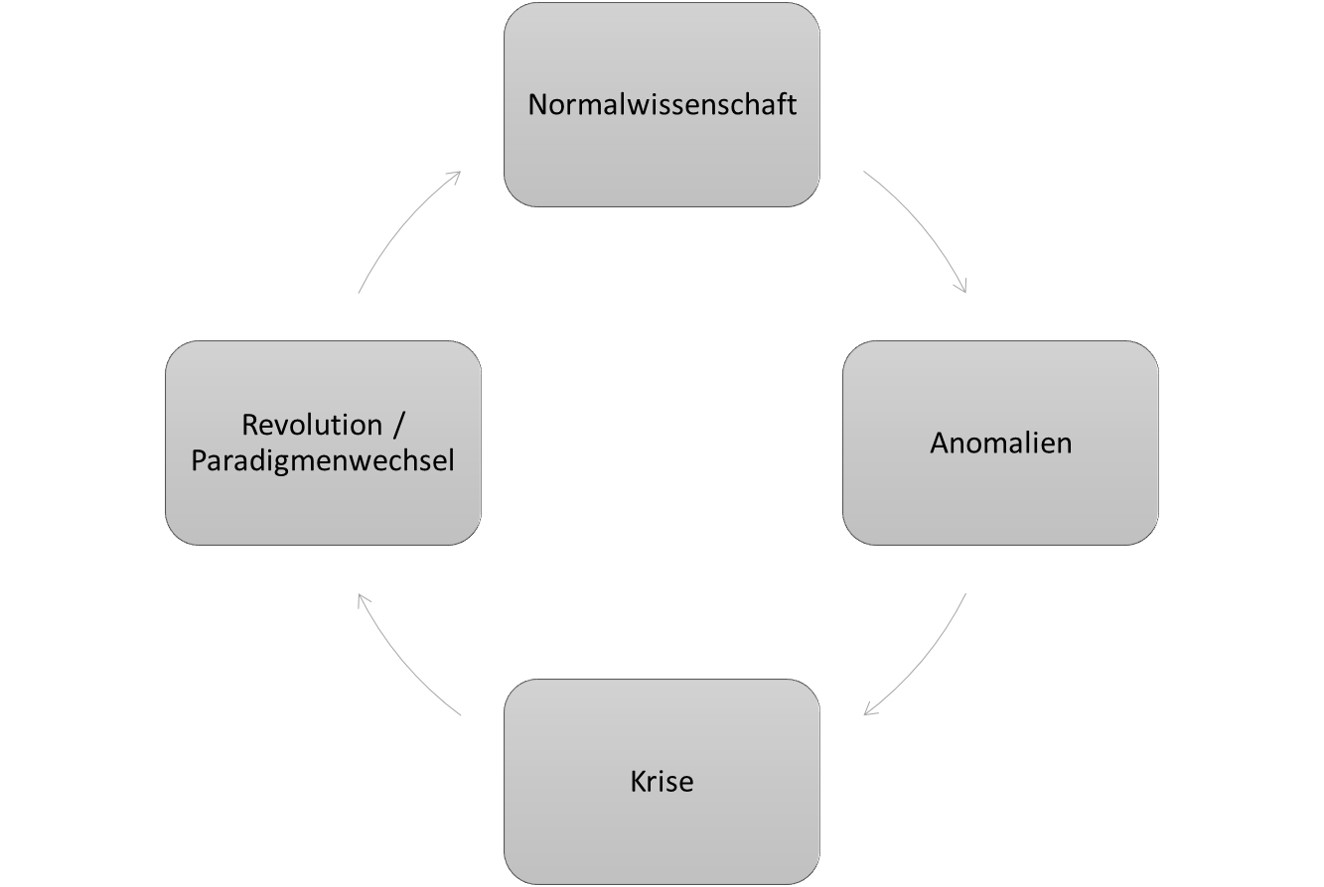
\includegraphics{images/paradigmenwechsel.jpg}

}

\caption{Wissenschaftliche Revolution nach {[}@Kuhn.19701996{]},
Darstellung in Anlehnung an {[}@Fiorentino2014-lr{]}}

\end{figure}%

Ein Paradigmenwechsel ist vergleichbar mit einem Kippbild die dem
Hase-Ente-Bild (\textbf{Abbildung 1}) wie es zum Beispiel
@Wittgenstein.1968 gezeichnet hat. Bis zu einem gewissen Punkt sind sich
alle einig, dass es ein Hase ist. Doch nach und nach kommen Erkenntnisse
und Perspektiven hinzu. Der Punkt wird überschritten, die Ente ist
anerkannt, und niemand würde es mehr für einen Hasen halten. Beim
Hase-Ente-Bild lässt sich natürlich beliebig hin und her springen. Beim
wissenschaftlichen \emph{Fortschritt} kommt neues Wissen hinzu und eine
Rückkehr ist nur noch schwer möglich.

\begin{figure}[H]

{\centering 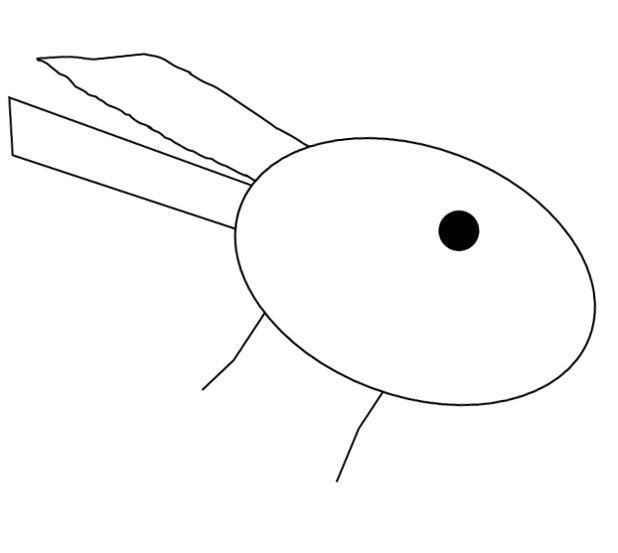
\includegraphics{images/entehase-01.jpg}

}

\caption{Hase-Ente-Kippbild frei nach Wittgenstein: Die Ausstülpungen
auf der linken Seite können entweder als Schnabel einer nach links
blickenden Ente oder als Ohren eines nach rechts blickenden Hasen
interpretiert werden.}

\end{figure}%

Forschende werden im Rahmen ihres Studiums oder einer Promotion von
Beginn an darin geschult, entsprechend des amtierenden Paradigmas mit
Befunden umzugehen.

\begin{tcolorbox}[enhanced jigsaw, bottomrule=.15mm, toprule=.15mm, opacitybacktitle=0.6, breakable, colback=white, coltitle=black, bottomtitle=1mm, toptitle=1mm, titlerule=0mm, title=\textcolor{quarto-callout-tip-color}{\faLightbulb}\hspace{0.5em}{Beim ersten Versuch klappt es nie: Paradigmenwechsel in der Psychologie}, rightrule=.15mm, arc=.35mm, opacityback=0, leftrule=.75mm, left=2mm, colbacktitle=quarto-callout-tip-color!10!white, colframe=quarto-callout-tip-color-frame]

Schon im Rahmen meines Studiums wurde ich geschult, mit dem amtierenden
Paradigma konform mit fehlgeschlagenen Replikationen umzugehen. Das fand
noch statt bevor sich die Replikationskrise herauskristallisierte. Bei
der ersten Studie, an der ich beteiligt war, replizierten wir
beispielsweise den Befund, dass bunte Mengen in ihrer Anzahl weniger
aussahen als einfarbige Mengen. Im Rahmen der Konsumentenpsychologie ist
das hinsichtlich Slogans wie ``viele viele bunte Smarties'' etwas
kontraintuitiv, es lässt sich aber gestaltpsychologisch plausibel
darlegen {[}@Redden.2009{]}. Nachdem eine Gruppe von Kommilitoninnen das
Gegenteil herausfand, nämlich dass \emph{bunte Smarties tatsächlich nach
mehr aussahen als einfarbige Smarties}, konnten wir in zwei eigenen
Folgestudien nichts vom beiden nachweisen. Egal ob sich die Smarties in
Teller, Tassen, oder Schalen, befanden, egal ob es blaue, rote, gelbe,
oder bunte Schokolinsen waren, egal ob Mengen geschätzt oder Smarties
aus großen Flaschen in Gefäße geschüttet wurden: Unsere Versuchspersonen
ließen sich von der ``Buntheit'' nicht beeinflussen. In den folgenden
Jahren durfte ich als Tutor dann weitere Replikationsversuche
durchführen. Der betreuende Professor und mein Mentor erklärte: Ich habe
es eigentlich noch nie erlebt, dass die Hypothese gleich beim ersten
Versuch bestätigt wird. Nach jedem Experiment ist man schlauer und weiß,
was man nächstes Mal besser machen muss. Es ist ganz natürlich, dass es
ein paar Versuche dauert, bis man weiß, wie sich die Hypothese
bestätigen lässt. Nachdem wir sechs Studien mit insgesamt 1383
Versuchspersonen durchgeführt hatten, die Autoren der Originalstudie um
Rat gebeten hatten, haufenweise Schokolinsen verzehrt hatten, und die
Hypothese über alle Studien hinweg nicht bestätigt wurde, hatte ich das
Vertrauen in den Befund verloren.

Ungefähr sechs Jahre später dachte ich während meiner Promotionszeit an
die Studien zurück und diskutierte mit dem Professor. Im Rahmen der
Replikationskrise war klar: Wenn man mehrere Experimente durchführt und
die Hypothese eigentlich falsch ist, wird alleine durch den Zufall ab
und zu trotzdem die Hypothese bestätigt. Das ist vergleichbar damit,
dass selbst eine faire Münze sechs Mal hintereinander auf derselben
Seite landen kann. Wenn man jedoch 10 Münzen jeweils sechs Mal wirft,
ist es nicht selten, dass eine der 10 Münzen sechs Mal auf derselben
Seite landet. Aus dieser Perspektive hat das Zitat, dass die Ergebnisse
beim ersten Versuch eigentlich nie so rauskommen, wie man es sich
wünscht, einen bitteren Beigeschmack: Wenn die Hypothese falsch ist, ist
es tatsächlich unwahrscheinlich, dass sie dennoch bestätigt wird. Nicht
aber, wenn viele Studien durchführt. Dann ist es sogar zu erwarten, dass
irgendwann eine Studie die Hypothese - auch wenn sie eigentlich falsch
ist (!) - bestätigt. Die Studien haben wir gemeinsam mit einigen
Beteiligten schließlich veröffentlicht {[}@Roseler.2020{]}.

\end{tcolorbox}

\subsection{Literatur}\label{literatur-4}

\chapter{Struktur der
Vertrauenskrise}\label{struktur-der-vertrauenskrise}

Im Gespräch über Präregistrierungen -- eine Methode zur Erhöhung der
Replizierbarkeit eines Befundes -- entgegnete ein Kollege: ``Schön und
gut, aber solange sich das System nicht ändert, wird sich an
Replikationsraten nichts ändern.'' Wie lässt sich dieser Einwand
verstehen? Zäumen (bzw. trensen) wir dazu das Pferd von hinten auf:
Spätestens seit dem Reproducibility Project Psychology (Open Science
Collaboration, 2015) ist den meisten Psycholog*innen klar, dass es große
Probleme bei der Replizierbarkeit von Befunden gibt. Woher kommen diese
genau? Ein wichtiges Problem ist hierbei der \emph{Publikationsbias},
womit gemeint ist, dass bei der Veröffentlichung von wissenschaftlichen
Berichten eine Auswahl getroffen werden muss und dadurch nur bestimmte
Ergebnisse publiziert werden (z.B. Ergebnisse, die eine bestimmte
Theorie stützen). Dadurch steht ein verzerrtes Bild der Realität. Oft
schreiben Wissenschaftler*innen sogar nur bestimmte Befunde zu Berichten
zusammen. ``Fehlgeschlagene Experimente'', also solche, bei denen eine
Hypothese nicht bestätigt oder eine Theorie nicht gestützt werden
konnte, landen in der Schublade (engl. \emph{File-Drawer-Problem};
@Rosenthal.1979; @Sterling.). In extremeren Fällen bedienen sich
Wissenschaftler*innen verschiedener größtenteils anerkannter Methoden,
die Daten so darzustellen, dass sie die Hypothese stützen oder tun so,
als ob das, was sich aus den Daten lesen lässt, von Beginn an die
Hypothese gewesen wäre (HARKing, @Parsons.2022). Aber was treibt
Personen, die sich vor allem für den Beruf wegen ihres Interesse an der
Funktionsweise der Welt (oder im Falle der Psychologie der
Funktionsweise des Menschen) und wegen Ihrer Suche nach Wahrheit
entschieden haben dazu, die Wahrheit zu unbewusst zu schönen oder sogar
bewusst zu manipulieren? Am Anfang des komplexen Prozesses, welcher zur
Replikationskrise geführt hat, steht das aktuelle wissenschaftliche
System: Ein Großteil der in der Wissenschaft beschäftigten arbeitet
unter extremem Druck und prekären Arbeitsbedingungen. Um nach ein bis
zwei Jahren eine Vertragsverlängerung zu erhalten, müssen Publikationen
von Artikeln in möglichst angesehenen Fachzeitschriften nachgewiesen
werden. Diese kriegt man durch besonders aussagekräftige und spannende
Ergebnisse. Das Anreizsystem der Wissenschaft belohnt also nicht
Wahrheit, Genauigkeit, Bescheidenheit, oder Transparenz, sondern vor
allem diejenigen Dinge, die nicht in der Hand eine*r Wissenschaftler*in
liegen: Spannende und eindeutige Ergebnisse {[}@Bakker.2012{]}.

Der Prozess von prekären Arbeitsbedingungen bis zur niedrigen
Replikationsrate ist hier veranschaulicht. In den folgenden Kapiteln
werden die Probleme und Lösungsansätze im Detail diskutiert.

\textbf{Abbildung 2}

\begin{figure}[H]

{\centering 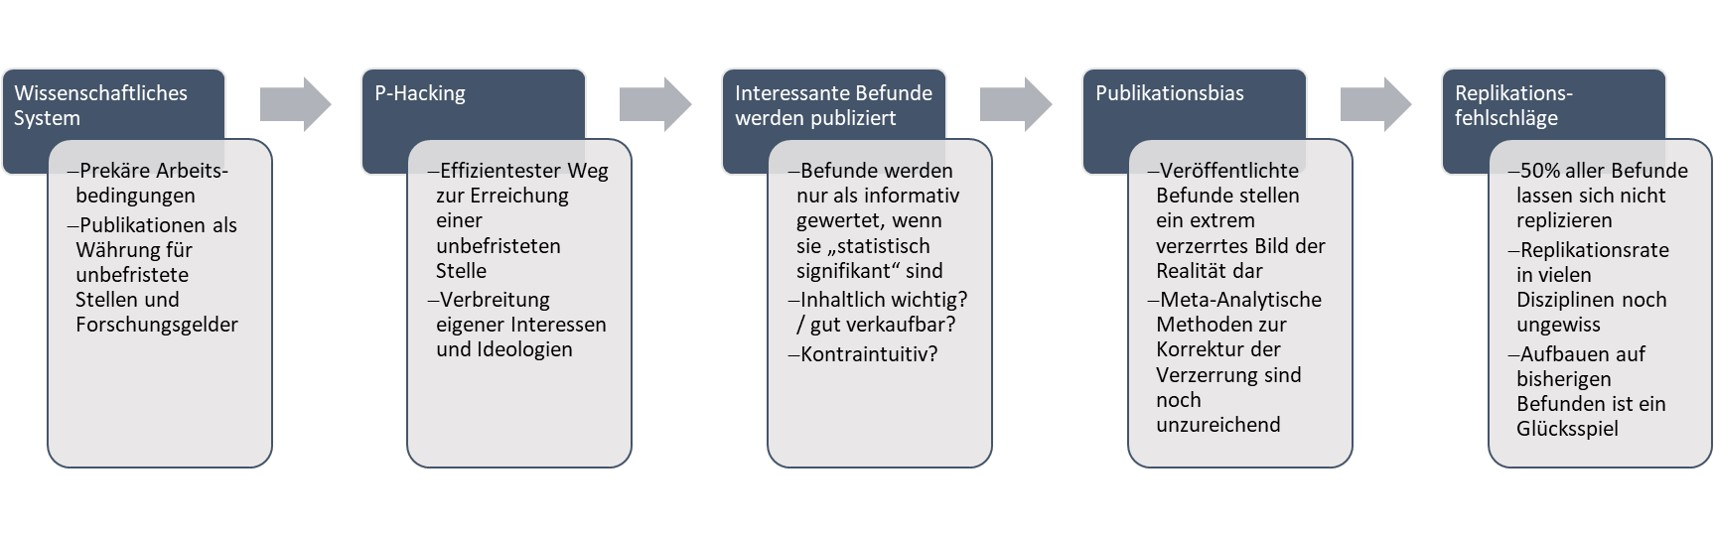
\includegraphics{images/struktur.jpg}

}

\caption{Das Anreizsystem der Wissenschaft als Ursache für
Replikationsfehlschläge}

\end{figure}%

\subsection{Literatur}\label{literatur-5}

\part{Probleme}

\part{Probleme, die im Rahmen der Revolution identifiziert wurden}

Im folgenden werden zahlreiche Probleme des Wissenschaftssystems erklärt
und aufgelistet. Manche der Probleme sind seit vielen Jahrzehnten
bekannt und andere erst seit wenigen Jahren. Es sei bei der Lektüre zu
beachten, dass es zu \emph{allen} diesen Problemen bereits
ausgearbeitete und teilweise auch ausgeführte Lösungsansätze gibt. Wie
die Lösungsansätze aussehen und welche Lösungen auf welche Probleme
zugeschnitten sind, wird ausführlich in \textbf{?@sec-lösungen}
erläutert.

\chapter{Probleme des Wissenschaftlichen
Systems}\label{probleme-des-wissenschaftlichen-systems}

\section{Probleme des Wissenschaftlichen
Systems}\label{probleme-des-wissenschaftlichen-systems-1}

Neben dem Idealbild davon, was Wissenschaft sein sollte oder wie sie
funktionieren sollte, existiert die Wissenschaft, wie sie in unser
Gesellschaftssystem integriert ist. Besonderheiten sind dabei, dass
Wissenschaftler*innen ihre Tätigkeit als Beruf ausüben, also Geld dabei
verdienen. Wie das Geld, das größtenteils aus Steuergeldern stammt,
verteilt werden soll entscheiden Gremien, die wiederum selbst aus
Wissenschaftler*innen bestehen (\emph{akademische Selbstverwaltung}).
Durch die hohe Arbeitsbelastung, gleichzeitig Wissenschaft zu betreiben
und zu verwalten, vereinfachen sich die Entscheider*innen die Arbeit und
verwenden zur Auswahl hochqualifizierter Personen Abkürzungen. So konnte
es passieren, dass die Währung in der Wissenschaft zum Großteil die
Anzahl der in Fachzeitschriften veröffentlichten Forschungsartikel
(\emph{Paper}) ist. Ein weiterer verwendeter Indikator ist die Anzahl,
in wie vielen weiteren wissenschaftlichen Artikeln auf die Forschung
einer Person verwiesen wird, also die Zitationszahlen. Vorbilder wie
Charles Darwin oder William James und selbst aktuelle Nobelpreisträger
hätten nach dem heutigen Maßstab keine Chance auf eine unbefristete
Stelle in der Wissenschaft - sie haben einfach nicht genug Paper
geschrieben. Viele der hier diskutierten Problemen, sind beispielsweise
in der Psychologie seit mehreren Jahrzehnten bekannt, sodass eine
Replikationskrise unabwendbar erschienen haben muss {[}@Cronbach.1991;
@Greenwald.1976{]}.

\subsection{Wissenschaft versus
Academia}\label{wissenschaft-versus-academia}

Während einige Natur- und Sozialwissenschaften in ihrer Anfangszeit oft
von Buchveröffentlichungen lebten und darin eine umfangreiche Basis von
meist einzelnen Personen erarbeitet wurde (z.B. Galileo Galilei für die
Physik oder William James für die Psychologie) stehen heutzutage
wissenschaftliche Fachzeitschriften im Fokus. Diese Zeitschriften sind
vergleichbar mit solchen, die es im Kiosk und im Supermarkt gibt, nur
bestehen sie halt aus (meist englischsprachigen) Artikeln, die
Wissenschaftler*innen verfasst haben und sind in vielen Fällen nur noch
online oder in Hochschulbibliotheken erhältlich. Forschende laden sich
dann einzelne Artikel aus den Zeitschriften aus dem Internet über das
Hochschulnetezwerk herunter und Bibliotheken haben Verträge mit Verlagen
und zahlen Geld, damit Universitätsangehörige Zugriff zu den Katalogen
haben. Jeder eingereichte Artikel befasst sich mit einer Fragestellung,
die von den Forschenden selbst festgelegt wurde (z.B. wie viele
psychologische Studien lassen sich im Mittel replizieren?). Darin werden
meistens Studien mit deren Ergebnissen berichtet. Vor der
Veröffentlichung werden die Artikel begutachtet (\emph{Review}) -- nicht
von Mitarbeitenden der Zeitschrift sondern von Kolleg*innen
(\emph{Peers}). Mit diesem \emph{Peer-Review} soll die Qualität von
Forschung sichergestellt werden. Üblicherweise wird dabei darauf
geachtet, dass die Schlussfolgerungen auf Basis der erhobenen Daten
gerechtfertigt sind, die Fragestellung klar beantwortet wird, der
Artikel verständlich ist, und die Befunde spannend oder überraschend
sind. Zeitschriften unterscheiden sich darin, welche Themen sie abdecken
(z.B. Sozialpsychologie, Konsumentenverhalten, Angewandte
Sportwissenschaft, usw.), wie streng das Peer-Review ist, und von wie
vielen Forschenden sie gelesen und zitiert werden. Wissenschaften sind
also stark integriert in ein System, das Forschenden und Verlagen
erlaubt, ein festes Gehalt zu verdienen.

\subsection{Prekäre Arbeitsbedingungen}\label{sec-arbeitsbedingungen}

Soweit der Rahmen: Wissenschaftler*innen forschen und teilen ihre
Ergebnisse meist in Form von \emph{Publikationen} wie
Zeitschriftenartikel- oder Buch-Veröffentlichungen. Was die Jobs in der
Wissenschaft (also vorwiegend an Hochschulen) angeht, so sind sie
hierarchisch strukturiert. Es gibt wenige unbefristete Stellen, meist
Professuren, und darunter befristete Stellen für Promovierende und
bereits promovierte \emph{Post Docs}. Wer in der Wissenschaft arbeitet,
befindet sich meistens in einem harten Konkurrenzkampf um eine der
wenigen unbefristeten Stellen {[}@Rahal.2023{]}. Der Hintergedanke ist
dabei, dass Konkurrenz zwischen Forschenden die Produktivität steigern
möge. Vom Start der Promotion\footnote{Prozess der Erlangung eines
  Doktorgrades/Doktortitles, je nach Disziplin und Hochschule durch das
  Verfassen eines Buches (Monografie) oder mehrerer Zeitschriftenartikel
  (kumulative Promotion)} bis zur Berufung auf eine Professur, also eine
der raren unbefristeten Stellen, dauern Verträge meistens nur ein bis
drei Jahre und haben oft einen Umfang von weniger als 100\%.
Gleichzeitig ist es unüblich ist, mit weniger als 40 Stunden pro Woche
innerhalb von den typischen drei Jahren die Promotion erfolgreich
abzuschließen. Während ein Großteil aller wissenschaftlichen
Veröffentlichungen auf Studien beruht, die im Rahmen von Doktorarbeiten
durchgeführt wurden, sind Doktorand*innen gleichzeitig diejenigen
Personen im System, die den geringsten Wert haben bzw. deren
Arbeitskraft am günstigsten ist. Forschende auf befristeten Stellen sind
also einem enormen Leistungsdruck ausgesetzt. Psychische Probleme wie
Burnout oder Depressionen sind unter Promovierenden weit verbreitet
{[}@Jaremka.2020; @Liu.2019{]}. Den Weg zur Professur schaffen vor allem
die Personen erfolgreich, die viele Artikel in prestigeträchtigen
Zeitschriften veröffentlichen. Durch die immense Arbeitsbelastung und
große Zahl an Artikeln, die bei Fachzeitschriften eingereicht werden,
ist keine Zeit mehr, Ergebnisse genau zu prüfen und nachzurechnen
{[}@Nuijten.2017{]}, sondern es wird vor allem darauf geachtet, wie
eindeutig die Ergebnisse die Fragestellung beantworten - oder genauer
gesagt: bestätigen {[}@GinerSorolla.2012; @Mynatt.1977{]}. Mit anderen
Worten: Es wird ausgerechnet der Teil der wissenschaftlichen Arbeit
belohnt, der nicht in der Hand der Forschenden liegt, nämlich die
Ergebnisse von Untersuchungen. Veröffentlichte Artikel und Prestige
statt Qualität {[}@Brembs.2018{]} sind ab dort die Währung der
Wissenschaft: Auf ihrer Basis wird entschieden, wer Forschungsgelder
erhält und auf Basis von Forschungsgeldern und Publikationen werden
Professuren vergeben. In den darüber entscheidenden
Berufungskommissionen lesen die Beteiligten üblicherweise nicht die
Artikel der Bewerbenden, sie zählen bloß, wie viele in welchen
Zeitschriften aufgelistet werden. Teilweise werden die Bewerber*innen
gebeten, Zitationszahlen anzugeben. Manche dieser Zahlen (z.B. Impact
Factor) gehören Unternehmen an und der Zugang muss über die Institution
erkauft werden.

Zu diesen verheerenden Problemen kommen außerdem systemische Probleme
der sexuellen Belästigung {[}@Hoebel.2022{]} und des Machtmissbrauches,
die in dem aktuell streng hierarchischen Aufbau des Systems nur
schwierig zu lösen sind (@Forster2018-up, siehe auch
\url{https://www.netzwerk-mawi.de/} und
\url{https://www.jmwiarda.de/2023/11/20/das-stille-leiden-der-betroffenen/}).
Berichten des Netzwerkes gegen Machtmissbrauch in der Wissenschaft
werden Fälle verschwiegen, und die schuldigen wechseln stillschweigend
die Universität, sodass das Problem nicht gelöst wird. Wer es dabei
besonders leicht hat, erklären @Elsherif.2022 anschaulich an dem
\emph{Academic Wheel of Privilege} (``Akademisches Rad der
Privilegierten''; S. 85; siehe auch
\url{https://www.psychologicalscience.org/observer/gs-navigating-academia-as-neurodivergent-researchers}).
Beispielsweise haben Doktorandinnen in den Niederlanden vor allem dann
schlechtere Noten als Doktoranden bekommen, wenn der
Promotionsausschuss, also die Gruppe an Professor*innen, die die
Promotion beurteilt, nur aus Männern bestand {[}@Bol2023-ij{]}.
Schwerbehindertenquoten weit unter den
\href{https://www.laborjournal.de/rubric/essays/essays2023/e23_09.php}{Quoten}
anderer Berufe kommen ebenfalls hinzu.

\subsection{\texorpdfstring{\textbf{Zu viel
Forschung}}{Zu viel Forschung}}\label{zu-viel-forschung}

Im Rahmen von Promotionen müssen Forschende in insgesamt 3-6 Jahren
zuzüglich Elternzeiten üblicherweise drei wissenschaftliche Artikel
veröffentlichen (bzw. in fairen Fällen drei
veröffentlichungs-\emph{würdige} Artikel vorweisen). Bei Post Docs
(siehe Section~\ref{sec-arbeitsbedingungen}) müssen es noch mehr sein.
Dass Personen vor und nach der Promotion jeweils maximal 6 Jahre an
Hochschulen angestellt sein dürfen ist gesetzlich festgelegt. Für die
weitere Qualifikation \emph{Habilitation}, für die eine ähnliche Zeit
angesetzt ist, sind zum Beispiel in der Psychologie circa 6 Artikel die
Daumenregel. Dabei spielt es eine nachrangige Rolle, wie umfangreich die
Artikel sind. Beispielsweise dauert die Durchführung einer Meta-Analyse,
in der bisherige Befunde zu einem bestimmten Thema systematisch
gesammelt und statistisch zusammengefasst bzw. verglichen werden, oft
mehrere Jahre. Eine Längsschnitterhebung kann je nach Forschungsfrage
sogar Jahrzehnte dauern. Im Kontrast dazu lässt sich eine
Querschnittserhebung über einen Online-Fragebogen in wenigen Wochen
durchführen. Eine Doktorandin, die eine einzige Meta-Analyse durchführt,
könnte damit nicht promovieren. Hätte sie stattdessen drei einfache
Online-Studien durchgeführt und einzeln veröffentlicht, wäre es
kein.\footnote{Hier ließe sich einwenden, dass einige Zeitschriften nur
  Artikel veröffentlichen, in denen mehrere Studien durchgeführt wurden.
  Das Ziel, nämlich die \emph{internale} Replikation der eigenen
  Befunde, verfehlen diese Zeitschriften damit deutlich. Stattdessen
  reizt es Forschende dazu an, mehrere Studien mit wenigen
  Versuchspersonen durchzuführen, statt eine Studie mit vielen
  Befragten.} Diese willkürlichen Vorgaben haben dazu geführt, dass sich
Wissenschaftler*innen alleine durch die Begutachtung der Artikel ihrer
Kolleg*innen einen enormen Arbeitsaufwand auferlegen, der den
wissenscchaftlichen Fortschritt behindert {[}@Hanson.2023{]}.

Zur Veranschaulichung des Aufgabenpensums nun ein Gedankenspiel:
Angenommen es gäbe 10 Wissenschaftler*innen, die gemeinsam 10 Artikel im
Jahr veröffentlichen würden - manchmal alleine, manchmal in einer Gruppe
- und jeder der Artikel würde von zwei Personen begutachtet, so müsste
jede*r zwei Artikel begutachten. Damit das System funktioniert, müsste
jede Person die Anzahl der im Schnitt veröffentlichten Artikel mal die
Anzahl der benötigten Gutachtenden begutachten. Bei 10
Veröffentlichungen pro Person und drei Gutachtenden wären es 10x3=30
Gutachten. Nun werden aber nicht alle Artikel von der Zeitschrift, bei
der sie eingereicht werden, veröffentlicht, noch werden sie sofort
veröffentlicht. Wissenschaftler*innen reichen ihre Artikel oft bei den
``hochrangigsten'' Zeitschriften ein. Nachdem dort mehrere
Gutachter*innen den Artikel geprüft haben, wird er abgelehnt
{[}@Jaremka.2020{]}. Im Mindestfall werden Revisionen angefordert,
welche oft eine weitere Runde Peer Review auslösen und nicht immer
werden Artikel danach veröffentlicht. Unsere Rechnung geht also nicht
auf: Nehmen wir \emph{vorsichtshalber} an, ein Artikel würde neun Mal
begutachtet (z.B. einmal drei Gutachtende, dann Ablehnung, dann erneut
drei Gutachtende, Revision, zweites Gutachten, Akzeptanz). Aus 10x3 wird
10x9, bei etwas Urlaubszeit also etwas mehr als zwei Gutachten pro
Woche, idealerweise bis zu zwei Arbeitstage. Bei dieser Rechnung bleibt
weniger Zeit für Lehre, Wissenstransfer, Betreuung von Studierenden oder
Promovierenden, Einwerbung von Forschungsgeldern, universitäre
Selbstverwaltung, usw. Durch die vielen zu publizierenden Artikel und
das strenge Review-System bürgt sich die Wissenschaft einen großen Berg
Arbeit auf -- einen der realistisch nicht machbar ist und unter dem am
Ende die Qualität der Forschung leidet. Beispielsweise fiel es weder den
Gutachtenden, noch den Herausgebern von Zeitschriften auf, dass in über
30 Artikeln mitten im Text „Regenerate response'' stand -- ein Satz, der
in OpenAIs ChatGTP Programm auf einem Knopf erlaubt, einen von einer
künstlichen Intelligenz erstellten Text umzuformulieren
(\url{https://retractionwatch.com/2023/10/06/signs-of-undeclared-chatgpt-use-in-papers-mounting/}).
In manchen Artikeln hieß es sogar „As an AI language model, I \ldots''
(\href{https://pubpeer.com/search?q=\%22As+an+AI+language+model\%2C+I}{https://pubpeer.com/search?q=``As+an+AI+language+model\%2C+I}``).
In einem Fall wurde der Artikel von dem Verlag Elsevier geändert, und
zwar nicht auf dem empfohlenen Weg\footnote{Ethische Richtlinien im
  Publikationsprozess sind zum Beispiel verfügbar über das Committee on
  Publication Ethics
  (\url{https://publicationethics.org/guidance/Guidelines}).} mittels
eines transparenten \emph{Errandum} oder \emph{Corrigendum}, also einer
öffentlichen Mitteilung über die Änderung und ihre Gründe, sondern ohne
Erklärung oder Zustimmung der Autor*innen
(\url{https://predatory-publishing.com/elsevier-changed-a-published-paper-without-any-explanation/}).

\subsection{Publish or Perish -- Veröffentlichen oder
Verenden}\label{publish-or-perish-veruxf6ffentlichen-oder-verenden}

Wer in der Wissenschaft arbeitet sollte die wichtigste Spielregel
kennen: Wer überleben will, muss Artikel veröffentlichen. Kurz:
Veröffentlichen oder Verenden (engl. \emph{publish or perish}). Zur
Promotion, Habilitation, Einwerbung von Forschungsgeldern, und zur
Berufung auf eine Professur sind Veröffentlichungen das oberste
Kriterium. Kennzeichen einer Währung ist, dass sich Dingen ein Wert
zuweisen lässt. Wie sieht der Wert in der Forschung aus?
Bibliometriker*innen entwarfen zur Beschreibung und zur Auswahl von
Zeitschriftenabonnements (also explizit \emph{nicht zur Bewertung})
verschiedener Forschungsgebiete verschiedene Kennzahlen, wie den Impact
Factor, oder Hirsch-Index. Beide Zahlen bestehen aus Verrechnungen
davon, wie oft Artikel je nach Zeitschrift oder je nach Person zitiert
wurden. Beispielsweise werden beim Journal Impact Factor die Gesamtzahl
der Zitationen in einem bestimmten Jahr durch die Anzahl der zitierbaren
Veröffentlichungen in Bezugsjahren (z.B. den 3 vorangegangenen Jahren)
geteilt. Zeitschriften werden mit hohen Impact Factors beworben und
erlauben teilweise nicht die Zitation von Kommentaren (bzw.
veröffentlichen Kommentare unter derselben Referenz wie
Originalstudien), um möglichst hohe Impact Factors zu erhalten. Sie
können natürlich auch entscheiden, ob sie den 3-Jahres- oder 2-Jahres
Impact Factor berichten. Berechnungsweisen unterscheiden sich außerdem
darin, auf Basis welcher Daten sie errechnet werden. Die Datenbank des
Journal Impact Factors gehört dem Unternehmen Clarivate Analytics und
ist nicht öffentlich zugängig. Das heißt, die genauen Zahlen lassen sich
nicht einfach nachrechnen und prüfen. Durch die wichtige und
intransparente Rolle von Zitationsmetriken ist wenig überraschend, dass
sie manipuliert werden (REF\hyperref[_msocom_7]{{[}LR7{]}},
\url{https://quantixed.org/2016/01/05/the-great-curve-ii-citation-distributions-and-reverse-engineering-the-jif/}).
Klar ist auch, dass Zitationsmetriken entweder gar nicht oder negativ
mit wissenschaftlicher Qualität zusammenhängen {[}@Brembs.2018;
\url{https://www.researchgate.net/publication/380433173_Inter-Rater_Reliability_in_Assessing_the_Methodological_Quality_of_Research_Papers_in_Psychology}
Table 3{]}. Zum Beispiel gab es das Problem, dass das Programm Microsoft
Excel Genomnamen als Datumsangaben erkannt hat, umformatiert hat, und
die eigentlichen Namen nicht mehr erkennbar waren. Somit waren Teile der
jeweiligen Ergebnisse
{[}nutzlos{]}(https://genomebiology.biomedcentral.com/articles/10.1186/s13059-016-1044-7\#:\textasciitilde:text=Indeed\%2C\%20the\%20number\%20of\%20papers,(3.8\%20\%25\%20per\%20year).
Dieses Problem kam vor allem bei angesehenen Zeitschriften vor. Sie
haben nichts dagegen unternommen, stattdessen wurde Excel nach ein paar
Jahren angepasst.

Neben Zeitschriften können auch Ranglisten von Personen erstellt werden.
Forschende aus Stanford veröffentlichten eine solche Liste der \emph{20
meistzitierten Forschenden.} Abgesehen davon, dass sie zum Missbrauch
verführt, enthält zahlreiche Fehler {[}@Abduh2023-sj{]} wie zum Beispiel
Forschende, die hunderte Jahre lang Artikel veröffentlicht haben -- vor
und nach ihrem Tod. Unternehmen, denen Verlage und andere Werkzeuge für
die Wissenschaft (z.B. Programme zur Verwaltung von Literatur) gehören,
sammeln darüber hinaus Daten über die Forschenden (z.B. welche Artikel
wie lange aufgerufen werden, welche Textpassagen markiert werden).
Teilweise werden Bibliotheken aufgefordert, Überwachungsprogramme von
Verlagen zu installieren. Die gesammelten Daten verkaufen die Verlage
dann zurück an die Forschenden. Diese Praxis gefährdet die
Wissenschaftsfreiheit, da Staaten Verlage auffordern können, die Namen
von Forschenden zu nennen, die zu politisch brisanten Themen forschen.
Die Initiative \href{https://stoptrackingscience.eu}{Stop Tracking
Science} setzt sich gegen das Verhalten ein.

Seit längerem wird für die verantwortungsvolle Verwendung dieser
Metriken plädiert {[}@Hicks.2015{]} und zahlreiche Universitäten und
Forschende tun sich zusammen um Bewertung von Forschung sinnvoll zu
gestalten (z.B. mittels der
\href{https://sfdora.org/read/read-the-declaration-deutsch/}{San
Francisco Erklärung zur Forschungsbewertung}). Wie sich Anreizstrukturen
und Karrierestatus auf wissenschaftliches Fehlverhalten auswirken, wird
mit gemischten Ergebnissen untersucht. Das Problem: Sobald es in einem
System ein klares Bewertungskriterium gibt, wird alles darauf
ausgerichtet (\emph{gaming the system}). Anreizstrukturen, die schlechte
Forschung zur Folge haben herrschen in Bezug auf Bildmanipulationen in
der Biologie laut @Fanelli2022-tx vor allem in China, weniger jedoch in
USA, Großbritannien, und Kanada.

Ein weiteres Produkt der \emph{Publish or Perish Struktur} ist, dass die
meisten in der Psychologie entwickelten Instrumente zur Messung von
Persönlichkeitseigenschaften nur wenige Male verwendet werden -- und das
auch hauptsächlich von ihren eigenen Entwickler*innen {[}@Elson.2023{]}.
@Elson.2023 plädieren: Psychologische Messinstrumente sind keine
Zahnbürsten! Ein noch extremeres Ausmaß ist bei sogenannten \emph{Paper
Mills} zu sehen {[}@vanNoorden.2023{]}: Personen erstellen dabei
automatisiert große Mengen von wissenschaftlichen Artikeln, ohne die
darin beschriebenen Untersuchungen wirklich durchzuführen.
Wissenschaftler*innen können dann Ko-Autor*innenschaften kaufen, um ihre
Anzahl an veröffentlichten Artikeln zu erhöhen und mehr Zitationen zu
bekommen. Je nach Zeitschrift werden diese Artikel nicht im Peer-Review
entlarvt. Es wird befürchtet, dass Käufer*innen solcher Artikel selbst
sehr erfolgreich werden können, selbst Herausgeber von Zeitschriften
werden, und sich dadurch selbst schützen, ertappt zu werden. Der genaue
Ausmaß des Paper-Mill-Problems ist unklar und weitgehend unerforscht
{[}@Byrne.2020{]}. Ein Indiz, mithilfe künstlicher Intelligenz erstellte
Artikel zu erkennen sind sogenannte \emph{tortured phrases
{[}@Cabanac.2021{]},} welche grammatisch korrekt sind, im üblichen
Sprachgebrauch jedoch selten vorkommen oder wenig Sinn machen.

\subsection{Flaschenhals-Hypothese und
Innovationsdrang}\label{flaschenhals-hypothese-und-innovationsdrang}

Namhafte wissenschaftliche Zeitschriften erhalten täglich unzählige
Einreichungen, veröffentlichen aber nur eine begrenzte Anzahl an
Artikeln. Sie müssen also streng selektieren, was begutachtet und
gegebenenfalls veröffentlicht wird. Weil das Ziel einer Zeitschrift ist,
viel gelesen zu werden, wählen Herausgeber*innen von Zeitschriften
diejenigen Artikel, welche möglichst großes Potenzial haben, bekannt und
viel zitiert zu werden {[}@GinerSorolla.2012{]}. Das betrifft zum
Beispiel Beiträge mit besonderen praktischen Implikationen,
überraschenden Befunden, oder besonders konsistenten Befunden. Studien,
deren Ergebnisse keine eindeutigen Schlüsse zulassen -- oder deren
Autor*innen mit zu großer Vorsicht Schlüsse ziehen -- kommen also nicht
infrage. In den Neurowissenschaften kommunizieren manche Zeitschriften
beispielsweise öffentlich, dass sie keine Replikationsstudien
veröffentlichen und nach Neuheit selektieren, während die meisten keine
Stellung dazu nehmen {[}@Yeung.2017{]}. In der Psychologie nahmen 2017
nur 33 von 1151 Zeitschriften Stellung dazu, dass sie Replikationen
akzeptieren {[}@Martin.2017{]}. Zwar werden innovative Befunde dann
häufiger zitiert, die Zeitschrift erhält also mehr Leser*innen, mehr
Einreichungen, und damit mehr Geld über Abonnements und
Veröffentlichungskosten. Vielzitierte Artikel lassen sich jedoch
schlechter replizieren als weniger zitiert {[}@SerraGarcia.2021{]} und
prestigereiche Zeitschriften sind Magneten für fragwürdige
Forschungspraktiken @{[}@Kepes.2022{]} und nachweisbar gleichwertige
oder sogar qualitativ schlechtere Forschung
{[}@Brembs.2018{]}.\hyperref[_msocom_10]{{[}LR10{]}}~

Wie kommt es dazu? Es ist die Rede von einem Flaschenhals
(\emph{Bottleneck}; viele Einreichungen aber wenige Veröffentlichungen).
Das führt gemeinsam mit dem Anreiz in eben solchen Zeitschriften zu
publizieren dazu, dass Forschende alle möglichen Mittel nutzen, um eine
Chance auf eine Publikation zu erhalten. In manchen Instituten gilt, wer
in einer bestimmten Zeitschrift veröffentlicht, erhält automatisch die
Bestnote auf die Promotion. Andere Institute erklären schon in der
Stellenausschreibung für eine Promotionsstelle, in welcher Zeitschrift
die Ergebnisse des Forschungsprojektes veröffentlicht werden müssen. Die
Tatsache, dass prestigereiche Zeitschriften \emph{Nature} oder
\emph{Science} vor allem Artikel mit klaren Botschaften
veröffentlichen\hyperref[_msocom_11]{{[}LR11{]}}, spornt also Forschende
an, klare Ergebnisse zu erschaffen. Passt mal ein Befund nicht zu der
geprüften Hypothese, wird er entweder manipuliert oder gar nicht
veröffentlicht und landet in der Schublade.

\subsection{\texorpdfstring{Schubladen-Problem\hyperref[_msocom_12]{{[}LR12{]}}~}{Schubladen-Problem{[}LR12{]}~}}\label{schubladen-problemlr12}

Seit mehreren Jahrzehnten ist bekannt, dass Wissenschaftler*innen vor
allem diejenigen Studien veröffentlichen, die ihre Theorien stützen
{[}@Rosenthal.1979; @Sterling.1959{]}. Im Extremfall hat jemand zum
Prüfen einer Theorie fünf Studien durchgeführt, in nur einer davon die
Theorie bestätigt, und nur diese veröffentlicht. Andere Forschende, die
dann die (veröffentlichte) Literatur durchsuchen, sehen nur die
``erfolgreiche'' Studie. Es entsteht der Eindruck, dass die Theorie
stimmt, während die Mehrheit der Studien diesen Schluss eigentlich nicht
nahelegt. Dass Studienergebnisse natürlichen, statistischen Schwankungen
unterliegen führt dazu, dass bei vielen Studien auch eine dabei sein
kann, die das gewünschte Ergebnis zeit. Durch das Schubladen-Problem
konnten sich ganze Forschungsstränge entwickeln, die seit dem
Bewusstsein für Replikationsstudien komplett ausgestorben sind
(Brockman, 2022).

Für \emph{Meta-Analysen}, also Studien, die bisherige Befunde
zusammenfassen, wurden bereits verschiedene Methoden entwickelt, die
Stärke des Schubladen-Problems (engl. \emph{File-Drawer-Problem}) zu
prüfen. Auch Methoden, diese Verzerrung zu korrigieren, existieren
bereits vielzählige {[}@Fisher.2017; @Hedges.1996; @Schimmack.2020;
@Simonsohn.2014; @vanAert.2018b{]}. Allerdings funktioniert keine der
Methoden in allen möglichen Szenarien {[}@Carter.2019{]}. Um eine
Veröffentlichung der fehlgeschlagenen Studien kommen Forschende also
nicht herum.

In der Medizin gibt es den besonderen Fall, dass alle dort
durchgeführten Studien öffentlich registriert
\hyperref[_msocom_13]{{[}LR13{]}}~werden müssen. Bei einer
Veröffentlichung muss dann eine Registrierungsnummer angegeben werden.
Über öffentliche Angaben zu registrierten Studien lässt sich somit
nachverfolgen, welche Personen, Institutionen, oder Länder wie viele
ihrer tatsächlich durchgeführten Studien veröffentlichen. Forschende in
Berlin haben dazu eine Website mit einem sogenannten interaktiven
\emph{Dashboard} entwickelt, um die darüber gesammelten Daten
durchsuchen und abbilden zu können {[}@Franzen.2023; @Riedel.2022{]}.
Auf \url{https://quest-cttd.bihealth.org/} ist nach aktuellem Stand
(Juli 2024) sichtbar, dass von allen registrierten Studien nur 46\%
innerhalb der folgenden zwei Jahre und 74\% innerhalb der folgenden fünf
Jahre veröffentlicht wurden. Personen, die sich für die Studien als
Versuchspersonen melden oder Drittmittelgeber erhalten somit Aufschluss
über die Größe der Schublade, in der die fehlgeschlagenen Studien und
die ``nicht so spannenden Ergebnisse landen''.

\subsection{Zugängigkeit von Wissen}\label{zuguxe4ngigkeit-von-wissen}

Durch die Einbindung von Forschung in das kommerzielle Verlagssystem
befindet sich ein Großteil der Wissenschaften in einem sozialen Dilemma,
das einen massiv eingeschränkten Zugang zum Wissen zur Folge hat. Das
vorherrschende Modell bei wissenschaftlichen Zeitschriften, die zum
Großteil Verlagen wie Springer, Elsevier, Sage, oder Taylor and Francis
angehören, ist ein Abonnement-Modell. Hochschul-Bibliotheken zahlen
Regelmäßig Geld an die Verlage, damit die Hochschul-Angehörigen (also
Studierende und Mitarbeitende) Zugriff auf die darin veröffentlichten
Arbeiten haben. Wer kein Abonnement hat, kann Artikel einzeln kaufen.
Versucht man, einen Artikel online herunterzuladen, ohne dass man sich
in einem Hochschulnetzwerk befindet, geht das nicht kostenlos: Der
Artikel befindet sich hinter einer Bezahlschranke (\emph{Paywall}). Soll
ein Artikel für alle frei zugänglich veröffentlicht werden (\emph{Open
Access},öffentlicher Zugang), kostet das extra, nämlich je Artikel
zwischen 2000€ und 9000€. Um Forschung also lesen zu können, müssen
Hochschulen Abonnements oder Artikel kaufen. Infolge dessen sind
finanziell schlechter ausgestattete Institutionen, Länder, oder sogar
gesamte Regionen wie der globale Süden in ihrer Teilnahme am
internationalen Wissenschaftsdiskurs systematisch benachteiligt.

Das soziale Dilemma besteht nun in der Schwierigkeit, dieses System zu
verändern. @Brembs.2023 beschreiben es wie folgt: Bibliotheken schließen
die Abos mit Verlagen ab, um Forschung an ihren Hochschulen zu
ermöglichen. Würden sie die Verträge kündigen, könnte das die Forschung
verlangsamen und die Stellung einer Hochschule verschlechtern.
Forschende können die namhaften Zeitschriften der kommerziellen Verlage
nicht boykottieren, da sie sonst ihre Karriere gefährden würden. Sie
sind darauf angewiesen, in prestigereichen Zeitschriften zu publizieren.
Zudem ist es extrem schwierig, das Verhalten von Millionen von
Forschenden, von denen die meisten viele Jahre lang mit dem aktuellen
System gelebt haben, schlagartig zu verändern. Die Zeitschriften, als
dritter Akteur in diesem Dilemma, profitieren von der Abhängigkeit und
können Preise beliebig steigen lassen. Abgesehen vom Markenwert der
Zeitschriften, also dem Ansehen und dem Vertrauen, das ihnen
fälschlicherweise {[}@Brembs.2018{]} entgegengebracht wird, tragen sie
zu diesem System fast nichts bei. Universitäten und Länder haben bereits
jetzt die Möglichkeit, Forschungsartikel online zu verwalten; die
Begutachtung und Qualitätssicherung geschieht durch freiwillige
Forschende und nicht durch Angestellte der Zeitschrift; und die
Formatierung der Artikel können Forschende wie an bestehenden
\footnote{Damit sind Zeitschriften gemeint, die Artikel ohne
  Abonnement-Zugang und ohne Paywall veröffentlichen, und zwar ohne
  Kosten für die Autor*innen.} ersichtlich ist {[}@Carlsson.2017{]}, mit
geringem Aufwand selbst übernehmen. Entsprechende Lösungen werden in
Section~\ref{sec-openaccess} erläutert.

\section{Vertiefende Informationen}\label{vertiefende-informationen}

Der kostenlose Film ``Paywall: The Business of Scholarship'' behandelt
das Thema Paywalls sowie den öffentlichem Zugang von wissenschaftlichem
Wissen: https://paywallthemovie.com/paywall

\section{Literatur}\label{literatur-6}

\chapter{Karriere in der
Wissenschaft}\label{karriere-in-der-wissenschaft}

Ein Beruf in der Wissenschaft setzt üblicherweise einen einschlägigen
Studienabschluss (Bachelor und Master) voraus und beginnt mit einer
Promotion. Im Rahmen der Promotion wird das wissenschaftliche Handwerk
erlernt und der Doktor*ingrad erlangt: Studien werden durchgeführt,
Daten analysiert, und Forschungsartikel veröffentlicht. In vielen Fällen
arbeiten Promovierende mit einer 50 -- 66\% Stelle als wissenschaftliche
Mitarbeiter*innen, begutachten für ihre Vorgesetzten Artikel und
Forschungsgelder-Anträge, schreiben eigene Anträge, verbringen mehrere
Monate im Ausland, erstellen, beaufsichtigen, und korrigieren Klausuren,
betreuen Abschlussarbeiten, und beteiligen sich an der universitären
Selbstverwaltung durch die Teilnahme an Sitzungen und Mitgliedschaften
bei Kommissionen. Zeitlich sind dabei bei Stellen oder Stipendien
üblicherweise drei Jahre angesetzt. Am Anfang meiner Promotion sagte man
mir, mit einer 40-Stunden-Woche schafft man es nicht, in der
vorgesehenen Zeit zu promovieren -- 50\% Gehalt für über 100\%
Arbeitszeit und einem befristeten Vertrag also. Verträge sind dabei
jedoch nicht immer auf die Zeit der Promotion befristet. Viele wissen
erst wenige Monate vor Vertragsende, wie viel Prozent Gehalt sie
erhalten, wie umfangreich die Lehrverpflichtung ist, und wie lange der
nächste Vertrag geht. Kurz: Die Arbeitsbedingungen sind nicht optimal
und man muss ein hohes Maß an Flexibilität mitbringen, wenn man sich für
den Weg in die Wissenschaft entscheidet.

\subsection{Doppelabhängigkeit}\label{doppelabhuxe4ngigkeit}

Für die Promotionsphase gibt es verschiedene Finanzierungsmöglichkeiten:
Über Unternehmen lässt sich berufsbegleitend promovieren oder Stipendien
zahlen über eine begrenzte Zeit Geld, das den Grunderhalt sichert (z.B.
1100€ über 36 Monate bei der Graduiertenförderung des Landes
Sachsen-Anhalt, dazu kommen noch zusätzliche Kosten für die
Sozialversicherung). Der häufigste Weg ist jedoch über eine Stelle als
wissenschaftliche*r Mitarbeiter*in. Dabei ist die vorgesetzte Person
diejenige Person, die auch die Promotionsarbeit bewertet. Die einem
auferlegte Korrektur der 120 Erstsemester-Klausuren steht dann im
Extremfall in Konflikt mit der Zeit, die für die Arbeit an der
wissenschaftlichen Studie benötigt wird. Promovierende hängen also
meistens von den betreuenden Professor*innen in Form der Beschäftigung
\emph{und} über die Bewertung ihrer Arbeit ab, was also als
\emph{Doppelabhängigkeit} bezeichnet wird.

\begin{tcolorbox}[enhanced jigsaw, bottomrule=.15mm, toprule=.15mm, opacitybacktitle=0.6, breakable, colback=white, coltitle=black, bottomtitle=1mm, toptitle=1mm, titlerule=0mm, title=\textcolor{quarto-callout-tip-color}{\faLightbulb}\hspace{0.5em}{Familienfeindliche Stipendien}, rightrule=.15mm, arc=.35mm, opacityback=0, leftrule=.75mm, left=2mm, colbacktitle=quarto-callout-tip-color!10!white, colframe=quarto-callout-tip-color-frame]

Unbefristete Stellen, Doppelabhängigkeit oder geringfügige Stipendien,
sowie Leistungsdruck haben klare negative Auswirkungen auf die
Gesundheit der Forschenden und damit auf die Qualität der Wissenschaft.
Wie sieht es mit Promotionsstipendien aus? Stipendien laufen oft 1 Jahr
mit Option auf Verlängerung oder bis zu 3 Jahre. Forschende, die direkt
nach der Schule und dem Studium promovieren, sind ca. 24 Jahre alt,
haben eventuell einen Partner, und wünschen sich eine Familie. Im Rahmen
ungewisser Vertragsverhältnisse ist das schwierig. Stipendien haben oft
keine Möglichkeit zur Elternzeit und müssen dann pausiert werden -- oder
sie laufen weiter und es wird keine zusätzliche Zeit angehängt. Sie
verbieten zusätzliches Einkommen, weshalb das Elterngeld dann auf den
dafür angesetzten Mindestbetrag fällt. Zusätzlich schreiben Sie vor,
dass die geförderte Person \emph{inklusive Ehepartner} ein bestimmtes
Maximalvermögen nicht überschreiten darf, sodass auch keine Finanzierung
durch mögliche Rücklagen klappt.

\end{tcolorbox}

\subsection{Depressionen, Burnout, und
\#IchbinHanna}\label{depressionen-burnout-und-ichbinhanna}

Fächerübergreifend hat sich als Antwort auf ein inzwischen gelöschtes
Erklärvideo vom Bundesministerium für Bildung und Forschung zum
Wissenschaftszeitvertragsgesetz (WissZeitVG) eine Bewegung unter dem
Hashtag \#IchbinHanna entwickelt, die die dortige sachliche Erklärung
(\url{https://www.youtube.com/watch?v=PIq5GlY4h4E}) und die
Arbeitsbedingungen in der Wissenschaft stark kritisiert. Es heißt „damit
auch nachrückende Wissenschaftlerinnen und Wissenschaftler die Chance
auf den Erwerb dieser Qualifizierung haben und nicht eine Generation
alle Stellen verstopft, dürfen Hochschulen und Forschungseinrichtungen
befristete Verträge nach den besonderen Regeln des WissZeitVG
abschließen. So kommt es zur Fluktuation und die fördert die
Innovationskraft''. 90\% aller Wissenschaftler*innen sind unbefristet
angestellt (\url{https://www.youtube.com/watch?v=H1wJmqpGhJc}).

Planungsunsicherheit und massiver Konkurrenzdruck fördern die
Innovationskraft? Das scheint unwahrscheinlich: Unter Forschenden
mentale Erkrankungen wie Burnout {[}@Jaremka.2020{]} und Anzeichen für
Angststörungen und Depression stark verbreitet. Einer Überblicksstudie
von @Satinsky.2021 zufolge, leiden zwischen 18 und 31\% der
Promovierenden unter Depressionen.

\begin{tcolorbox}[enhanced jigsaw, bottomrule=.15mm, toprule=.15mm, opacitybacktitle=0.6, breakable, colback=white, coltitle=black, bottomtitle=1mm, toptitle=1mm, titlerule=0mm, title=\textcolor{quarto-callout-caution-color}{\faFire}\hspace{0.5em}{Wer hilft?}, rightrule=.15mm, arc=.35mm, opacityback=0, leftrule=.75mm, left=2mm, colbacktitle=quarto-callout-caution-color!10!white, colframe=quarto-callout-caution-color-frame]

Schnelle Hilfe bei psychischen Problemen leistet beispielsweise das
Krisentelefon der
\href{https://www.telefonseelsorge.de}{TelefonSeelsorge}. Manche
Universitäten haben spezifische Anlaufstellen, Städte haben häufig
örtliche Psychotherapie-Ambulanzen und Beratungsstellen.

\end{tcolorbox}

\subsection{Top-Down-Wandel}\label{top-down-wandel}

Diejenigen, die das System ändern können, also alle mit unbefristeten
Verträgen, leiden nicht mehr unter ihm. Für diejenigen, die unter dem
System leiden, ist es unklug, das System ändern zu wollen und sich an
die Professor*innen zu wenden, denn das sind die Leute, die über ihren
späteren Verbleib in der Wissenschaft im Rahmen von
Berufungskommissionen bei der Entscheidung der Vergabe von Professuren
entscheiden. Im Extremfall kann das dazu führen, dass jemand Kritik an
Arbeiten von Wissenschaftler*innen in höheren Positionen aus Angst, die
eigenen Chancen auf eine Professur zu schmälern, zurückfährt. Auf der
anderen Seite haben Professor*innen bewiesen, dass sie sehr gut nach den
Spielregeln spielen können. Zuzugeben, dass sie eine der seltenen und
heiß begehrten Stellen nicht über Qualität sondern Quantität ihrer
Forschung erhalten haben, hieße, sich selbst abzuwerten.

\subsection{Literatur}\label{literatur-7}

\chapter{Probleme der wissenschaftlichen
Methoden}\label{probleme-der-wissenschaftlichen-methoden}

Im Alltagsdenken herrscht noch oft der Mythos, dass Wissenschaft sich
von Nicht-Wissenschaft durch \emph{die wissenschaftliche Methode}
unterscheide. Das ist falsch {[}@Feyerabend.19752002{]}. Zwar
unterscheidet sich wissenschaftliches Wissen von alltäglichem Wissen
(und auch Religion) durch einen höheren Grad an Systematizität
{[}@HoyningenHuene.2013{]}, allerdings gibt es weder eine einzige noch
eine konstante wissenschaftliche Methode. Methoden haben sich
stattdessen über die Zeit gewandelt, und das ist auch gut so. Neue
Technologien ermöglichen beispielsweise in der Physik hochpräzise
Messungen mittels Elektronenlaser, in den Geschichtswissenschaften
3D-Scans von Artefakten, die sonst nur wenige sehen würden, oder in den
Sozialwissenschaften Datenbanken mit freiwillig bereitgestellten und
anonymisierten Chatverläufen (\url{https://db.mocoda2.de/c/home}).

So wie ein Hammer und andere Werkzeuge nicht gut oder schlecht sind, so
sind auch Methoden nicht gut oder schlecht, nicht richtig oder falsch,
sondern sie werden \emph{angemessen und korrekt} verwendet oder
missbraucht. Statt Missbrauch ist in den Sozialwissenschaften von
fragwürdigen Forschungspraktiken (\emph{Questionable Research
Practices}), kurz QRP, die Rede. Sie erlauben Wissenschaftler*innen
Befunde zu generieren, die sie wollen. Im Folgenden werden verbreitete
und oft angewandte {[}@John.2012{]} Techniken vorgestellt (für einen
Überblick über die Forschung dazu in den letzten 50 Jahren, siehe auch
@Neoh.2023).

\subsection{Exploratorische versus konfirmatorische
Forschung}\label{exploratorische-versus-konfirmatorische-forschung}

Zum Verständnis der fragwürdigen Forschungspraktiken (QRP) ist eine
wichtige forschungstechnische Unterscheidung unabdingbar: Wie bei einem
Spaziergang kann eine wissenschaftliche Untersuchung erkundend oder
zielgerichtet sein. Mal wird frei durch die Gegend spaziert und dabei
neue Entdeckungen gemacht, mal ist das Ziel und die Route klar und im
Vorhinein bestimmt. Im wissenschaftlichen Kontext ist die Rede von
exploratorischer und konfirmatorischer Forschung. Bei der Exploration
stehen höchstens die Forschungsfrage und grobe Züge der Methode fest,
bei einem konfirmatorischen Test ist alles durchdacht: Vorgehen,
mögliche Ergebnisse, sowie Erklärungsansätze für jedes mögliche
Resultat. Es wird dann eine spezifizierte Hypothese mit der
dazugehörigen Theorie bestätigt oder eben nicht. Kein Vorgehen ist dem
anderen überlegen. Üblicherweise beginnen Untersuchungen in einem bisher
wenig erschlossenen Gebiet mit Exploration, während mehr vorhergehende
Forschung mit klareren Erwartungen einhergeht. Es sei dazu gesagt, dass
es sich hier um Extremtypen von Forschung handelt, die ein Spektrum
bilden. Es erlauben außerdem erst beide Ansätze zusammen
Erkenntnisgewinn. Im Rahmen des hermeneutischen Zirkel, (einfach gesagt
``dem Kreis des Verstehens'') wird aus einzelnen Beobachtungen eine
allgemeine Gesetzmäßigkeit formuliert (\emph{Induktion}) und diese
Gesetzmäßigkeit wird im Anschluss bei weiteren Einzelbeobachtungen
geprüft (\emph{Deduktion}). Die Deduktion kann je nach Gesetzmäßigkeit
logisch notwendig sein, denn es wird von Prämissen auf eine Konklusion
geschlossen. Wenn beide Prämissen korrekt sind, muss also auch die
Schlussfolgerung korrekt sein. Die Induktion ist keine Notwendigkeit
(siehe \emph{Induktionsproblem}, @Hume.17482011).

\begin{figure}[H]

{\centering 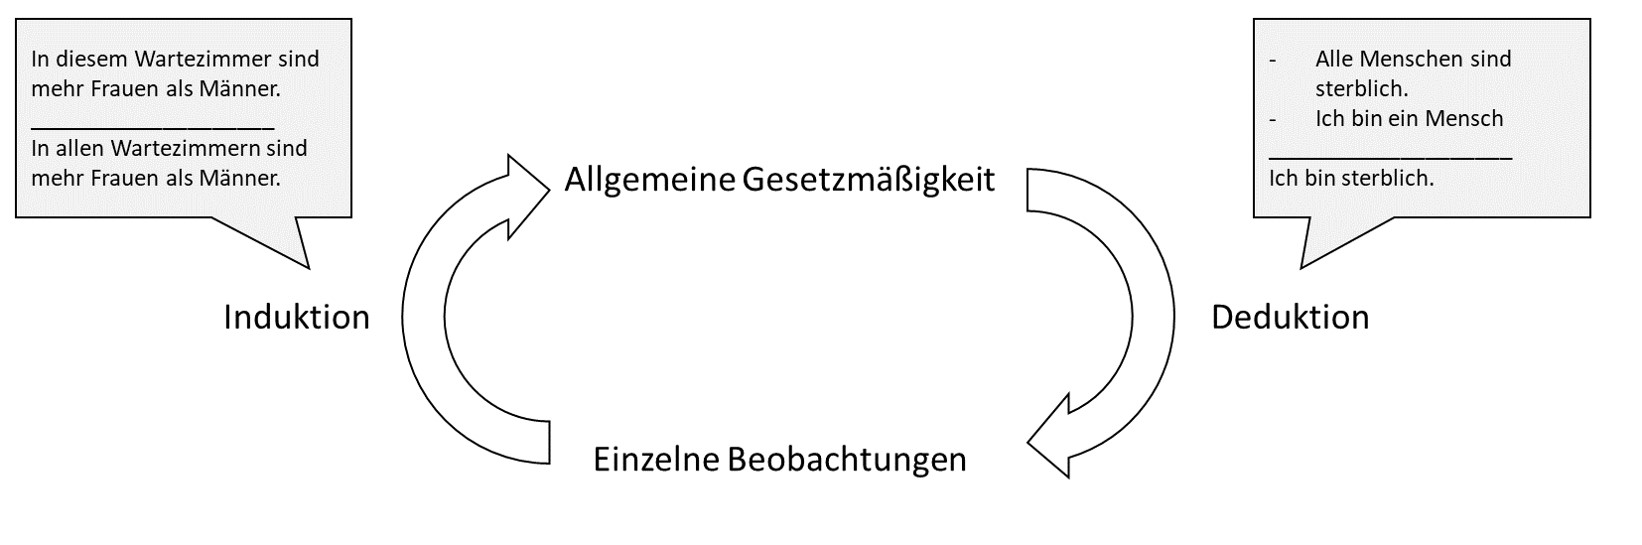
\includegraphics{images/hermeneutischerzirkel.jpg}

}

\caption{Hermeneutischer Zirkel}

\end{figure}%

Problematisch wird es, wenn exploratorische Forschung als
konfirmatorische kommuniziert wird, also so getan wird, als hätte eine
Einzelbeobachtung eine bereits formulierte Gesetzmäßigkeit bestätigt,
statt sie bloß inspiriert. Diese Art Unlogik heißt Zirkelschluss: Die
Gesetzmäßigkeit gilt wegen der Beobachtung. Und die Beobachtung
entspricht der Gesetzmäßigkeit.

\textbf{Abbildung Z}

\emph{Skizziertes Vorgehen bei explorativer (a) versus konfirmatorischer
(b) Forschung. Exploratives Vorgehen ist nicht zielgerichtet, die
Richtung kann sich ändern, und ist manchmal mit unvorhergesehenen
Ergebnissen verbunden. Konfirmatorisches Vorgehen bildet oft einen engen
und kontrollierten Ausschnitt eines Sachverhaltes ab.}

\subsubsection{Methoden der
Datengenerierung}\label{methoden-der-datengenerierung}

Wissenschaftliche Disziplinen bedienen sich für gewöhnlich vieler
verschiedener Methoden. Idealerweise sind Erkenntnisse unabhängig von
der Methode, die zu ihrer Entdeckung geführt hat und verschiedene
Methoden führen zur selben Erkenntnis. Typische sozialwissenschaftliche
Methoden sind die Befragung mittels standardisiertem Fragebogen,
Verhaltensbeobachtung mittels Kameraaufzeichnungen und anschließender
Kodierung von Verhaltensweisen durch mehrere Personen, die den
Untersuchungszweck nicht kennen, indirekte Methoden
{[}@Schimmack.2019{]}, bei welchen etwas anderes gefragt wird, als was
gemessen werden soll, Verhaltensmessungen wie Blickrichtungsmessung
(\emph{eye tracking}), oder Simulationsstudien, mittels derer zum
Beispiel Verkehrsflüsse auf Basis vorher festgelegter Prinzipien per
Computer berechnet werden oder Panikattacken vorhergesagt werden
{[}@Robinaugh.2021{]}. Diese Methoden generieren fast immer Daten, also
beispielsweise eine Tabelle, in der je Beobachtungseinheit (z.B. je
Versuchsperson) in mehreren Spalten Daten festgehalten werden und diese
Daten werden fast immer statistisch ausgewertet. Die Notwendigkeit einer
solchen Auswertung ergibt sich daraus, dass die Beobachteten
Gesetzmäßigkeiten keine absoluten Gesetze im Sinne von „alle männlichen
Babys wiegen mehr als alle weiblichen Babys'' sind, sondern statistische
Regelmäßigkeiten im Sinne von „im Mittel wiegen kurz nach der Geburt
männliche Babys ein paar hundert Gramm mehr als weibliche Babys, aber
nicht jedes männliche Baby wiegt mehr als jedes weibliche Baby'' sind
(siehe Abbildung X). Ein Vergleich von Körpergrößen nach Geschlecht ist
über
\href{https://de.statista.com/statistik/daten/studie/1825/umfrage/koerpergroesse-nach-geschlecht/}{Statista}
zu sehen.

\textbf{ABBILDUNG X}

\emph{Statistische Phänomen; männliche babys vs.~Weibliche babys}

\begin{tcolorbox}[enhanced jigsaw, bottomrule=.15mm, toprule=.15mm, opacitybacktitle=0.6, breakable, colback=white, coltitle=black, bottomtitle=1mm, toptitle=1mm, titlerule=0mm, title=\textcolor{quarto-callout-note-color}{\faInfo}\hspace{0.5em}{Statistische Signifikanz}, rightrule=.15mm, arc=.35mm, opacityback=0, leftrule=.75mm, left=2mm, colbacktitle=quarto-callout-note-color!10!white, colframe=quarto-callout-note-color-frame]

Eine der am weitesten verbreiteten Methoden in den Sozialwissenschaften
(und auch darüber hinaus) ist Statistik, genauer
\emph{Inferenzstatistik}. Dabei wird von einer begrenzten Menge von
Beobachtungen (z.B. ausgefüllte Fragebogen von 100 Personen) auf alle
möglichen Beobachtungen (z.B. alle Menschen) verallgemeinert.
Untersuchte Zusammenhänge sind selten eindeutig, es gibt aber häufig
statistische Regelmäßigkeiten. Charakteristisch ist dabei ein gewisses
\emph{Zufallselement}. Wiegt man ein kürzlich geborenes männliches und
weibliches Baby, dann ist die Wahrscheinlichkeit sehr hoch, dass das
männliche Baby mehr wiegt. Es kommt aber auch häufig vor, dass das nicht
der Fall ist. Ähnlich verhält es sich bei einer fairen Münze, also einer
die im Mittel gleich häufig auf Kopf und auf Zahl landet: Dass sie bei
insgesamt vier Würfen immer auf Kopf landet ist unwahrscheinlich, dass
sie 1 oder 2 Mal auf Kopf landet, es kommt aber durch aus vor (nämlich
in 12,5\% aller Fälle, in denen eine faire Münze vier Mal hintereinander
geworfen wird).

Inferenzstatistische Tests gehen nun davon aus, dass bei der Betrachtung
eines statistischen Zusammenhanges (z.B. Geschlecht und Geburtsgewicht,
Körpergewicht und Größe, Bildungsniveau der Eltern und Bildungsniveau
der Kinder) „nur der Zufall am Werk ist'' {[}@Roseler.2022f{]}. Unter
der Annahme wird berechnet, wie häufig ein beobachteter Zusammenhang mit
der beobachteten Stärke vorkommen würde, wenn \emph{eigentlich} kein
Zusammenhang vorliegen würde. Also zum Beispiel „dass eine faire Münze
vier Mal auf Kopf landet, passiert in 12,5\% aller Fälle''. Bei sechs
Würfen wären es 1,5625\%. Die Kunst des statistischen Schließens besteht
nun darin, den Punkt zu finden, ab dem Forschende davon ausgehen, dass
der Zufall nicht am Werk war, weil die berechnete Wahrscheinlichkeit so
gering ist. Konventionell liegt dieser bei 5\%, für neue Befunde
manchmal bei 0,5\% (Benjamin et al., 2018), und in besonders prekären
Fällen noch niedriger. Fachtechnisch wird von einem \emph{Alpha-Niveau}
oder einem \emph{Signifikanzniveau} gesprochen und die berechnete
Wahrscheinlichkeit heißt \emph{p}-Wert. P-Werte unter 5\% werden
\emph{statistisch signifikant} oder \emph{auf dem 5\%-Niveau
signifikant} bezeichnet. Forschende würden also sagen, dass eine Münze
\emph{nicht} fair ist, wenn sie sechs Mal hintereinander auf Kopf landet
(sogar schon bei fünf Mal, was in 3,125\% der Fälle vorkommt). Dabei
nehmen sie in Kauf, dass sie, wenn die Münze eigentlich doch fair ist,
in 5\% aller Fälle falsche Schlüsse ziehen.

Auf der anderen Seite ist es durchaus möglich, dass eine Münze nicht
fair ist, zum Beispiel in 60\% der Fälle auf Kopf landet und in 40\% auf
Zahl.~

\begin{figure}[H]

{\centering 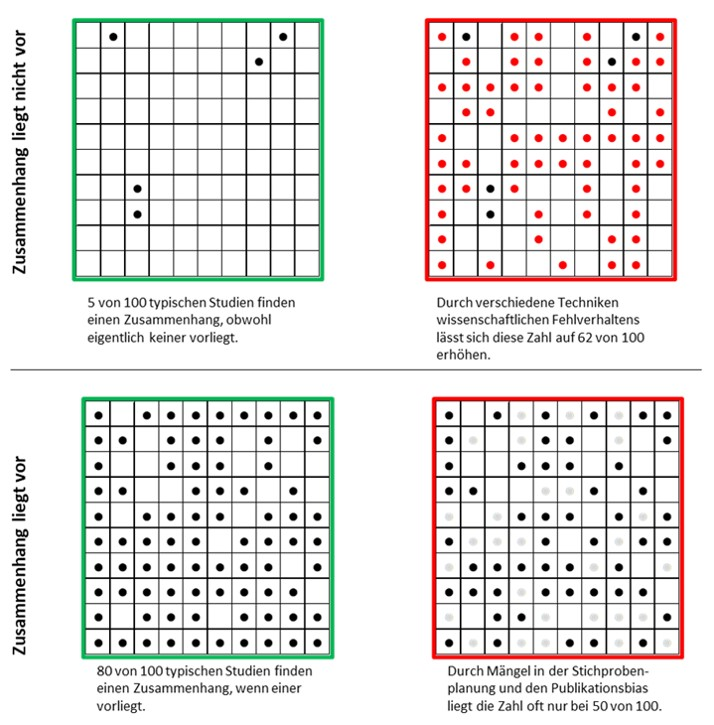
\includegraphics{images/freiheitsgrade.jpg}

}

\caption{Eine einzelne Studie führt noch nicht zu sicherer Erkenntnis.
Auch, wenn ein untersuchter Zusammenhang nicht vorliegt, kann er in
Daten zufällig aufscheinen. Und auch, wenn eigentlich ein Zusammenhang
vorliegt, kann dieser in den Daten durch Zufallsschwankungen nicht zu
erkennen sein. Mithilfe von Open Science Praktiken soll der Zustand in
den linken Kästen wiederhergestellt werden. Aus Röseler,~L. (2021).
Wissenschaftliches Fehlverhalten {[}Abbildung{]}. https://osf.io/uf7gz/.
Lizenziert unter CC BY-Attribution International 4.0.}

\end{figure}%

\end{tcolorbox}

\subsection{\texorpdfstring{Freiheitsgrade von Forschenden
(\emph{Researchers' Degrees of
Freedom})}{Freiheitsgrade von Forschenden (Researchers' Degrees of Freedom)}}\label{freiheitsgrade-von-forschenden-researchers-degrees-of-freedom}

Vollständige Studien mehrfach durchzuführen ist sehr aufwändig. Obwohl
es ein relativ sicherer Weg zu signifikanten P-Werten ist, gibt es
weitaus sparsamere Lösungen. Die meisten Analysen sind um ein vielfaches
komplexer als die oben beschriebene Münzwurfstudie. Betrachten wir den
immer noch sehr einfachen Signifikanztest für einen
Korrelationskoeffizienten. Der Koeffizient ist eine Zahl zwischen -1 und
1 und beschreibt die Art des Zusammenhanges zwischen zwei Variablen
(z.B. Einkommen und Lebenszufriedenheit). 0 bedeutet, dass kein
Zusammenhang vorliegt, positive Werte bedeuten, dass wenn die eine
Variable hohe Werte hat, dann hat auch die andere hohe Werte, und
negative Korrelationen bedeuten, dass wenn eine Variable hohe Werte hat,
dann hat die andere Variable eher niedrige Werte. In Abbildung X sind
verschiedene Korrelationen dargestellt.

\textbf{Abbildung X: Verschiedene Zusammenhänge zwischen zwei Variablen
und deren Korrelationskoeffizienten (simulierte Daten).}

Obwohl es sich hierbei um einen sehr einfachen Test handelt, bringt er
viele Entscheidungen mit sich. Selbst nach der Datenerhebung muss
entschieden werden: Welche der befragten Personen werden für den Test
verwendet? Sollen Personen ausgeschlossen werden und falls ja, warum
(z.B. extreme Werte oder unplausible Werte)? Wie werden die Werte der
Variablen berechnet? Welche Art der Korrelation soll verwendet werden
(z.B. Bravais-Pearson, Kendall, oder Spearman)? Gibt es eine Erwartung
der Richtung der Korrelation (Gerichtetheit der Hypothese)?

Diese Fragen entsprechen Freiheitsgraden -- Forschende sind also
dahingehend flexibel, welche Optionen sie wählen. Keine der Optionen ist
per se allen anderen überlegen und jede Entscheidung lässt sich in einem
gewissen Rahmen rechtfertigen. Das Problem dieser Flexibilität ist, dass
die Ergebnisse von ihr abhängen und je nach den Entscheidungen kann das
Ergebnis eine positive, negative, oder keine Korrelation bedeuten. Je
komplexer die Untersuchung und das statistische Verfahren ist, desto
größer ist auch die Flexibilität bei der Datenanalyse. An sich sind
diese Freiheitsgrade nichts Schlechtes, problematisch wird es bloß dann,
wenn nur diejenigen Ergebnisse dargestellt werden, die sich gut
veröffentlichen lassen oder zu den Überzeugungen der Forschenden passen.
Dieses Vorgehen heißt HARKing (hypothesizing after the results are known
= Hypothesen aufstellen, nachdem die Ergebnisse bekannt sind) und stellt
einen Zirkelschluss dar. Die Hypothese, die geprüft wurde, stammt aus
den Daten, die sich natürlich bestätigen. Verschiedene Lösungswege
erlauben auch die Reduktion oder komplette Auslöschung von
Freiheitsgraden (z.B. Präregistrierung, siehe Kapitel XXX). Auch ist es
möglich, das Vorgehen als explorativ, also nicht vorher durchdacht und
vorbestimmt, zu kommunizieren.

Im Datenanalyseprozess wird die Analogie des „garden of forking paths''
verwendet. In einem vereinfachten (!) Beispiel in Abbildung 4 haben wir
3x4x4x4 = 192 verschiedene Ergebnisse, die das gesamte Spektrum der
Schlussfolgerungen abdecken werden -- egal, ob unsere Hypothese stimmt
oder nicht.

\begin{figure}[H]

{\centering 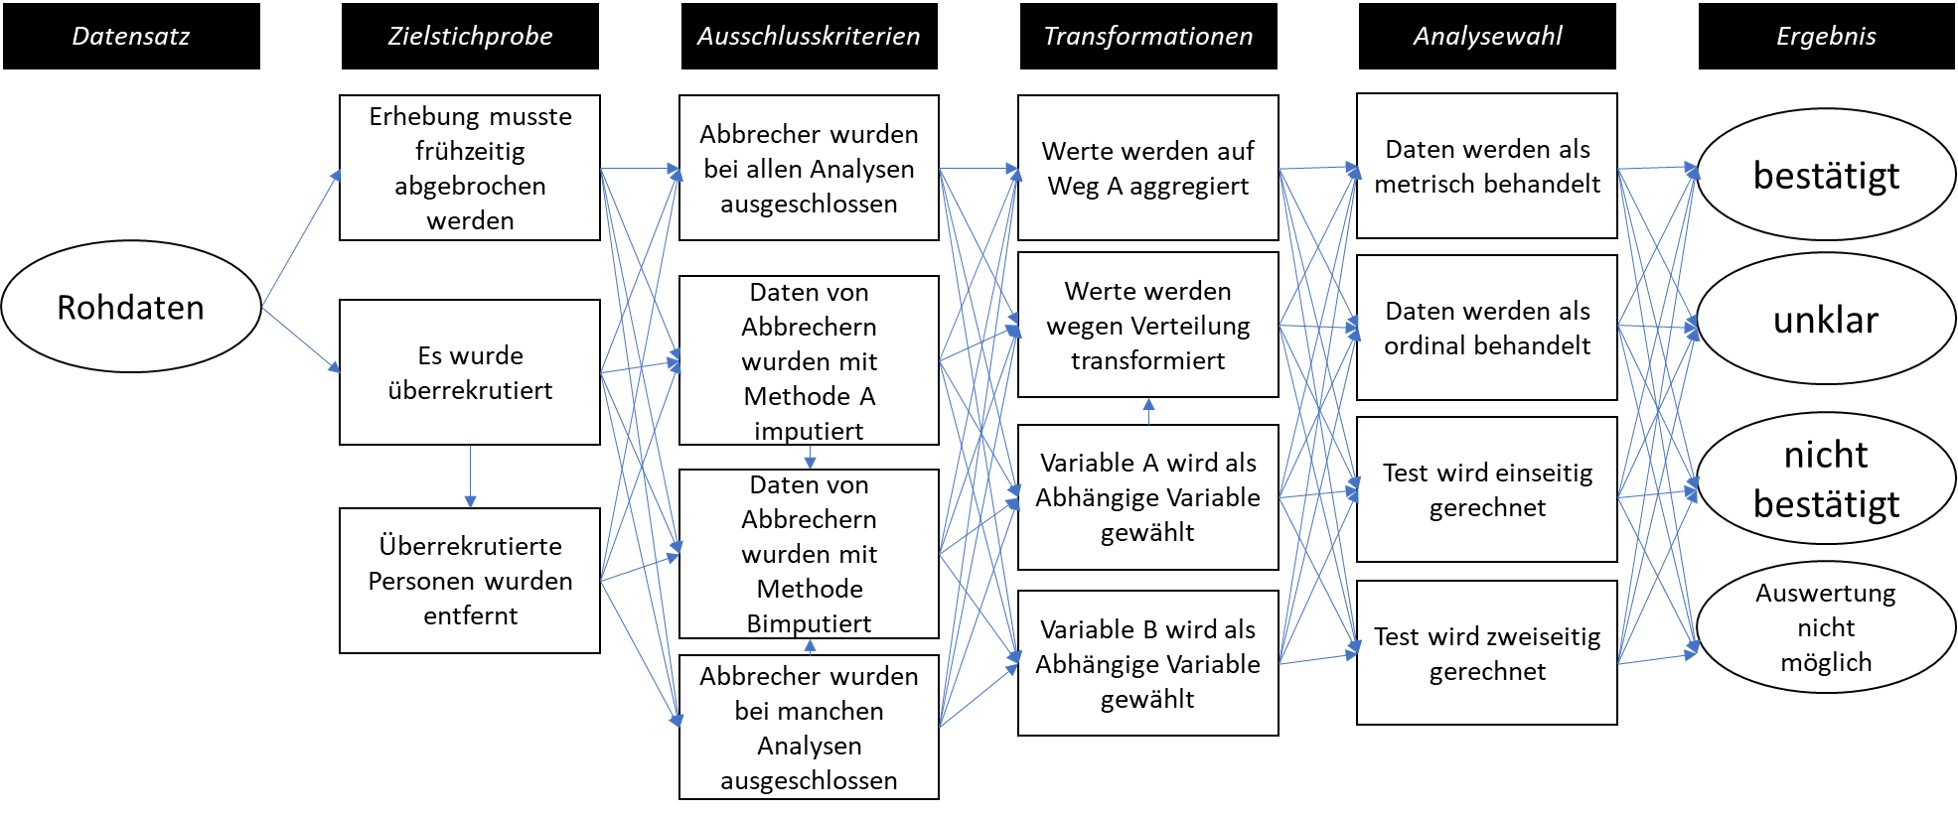
\includegraphics{images/gardenofforkingpaths.jpg}

}

\caption{192 verschiedene Wege von einem Datensatz zum (gewünschten)
Ergebnis}

\end{figure}%

\hyperref[_msocom_4]{{[}LR4{]}}~

Demonstrationen des garden of forking paths existieren für
verschiedenste Felder und wurden bereits für Evolutionsbiologie
{[}@Gould.2023{]}, Sozialpolitik {[}@Breznau.2022{]},
Strukturgleichungsmodelle (REF\hyperref[_msocom_5]{{[}LR5{]}}~), und
Sprachanalysen {[}@Coretta.2023{]} nachgewiesen.

\subsection{Tippfehler}\label{tippfehler}

Häufig werden Daten mittels fortgeschrittener Programme ausgewertet und
die Ergebnisse werden dann mühselig in den Bericht übertragen. Hierbei
entstehen schnell Tippfehler. @nuijten2016prevalence erstellten einen
Algorithmus, der automatisch berichtete Signifikanztests erkennt,
nachrechnet, und Inkonsistenzen zurückmeldet. Dabei fanden sie heraus,
dass in großen Psychologiezeitschriften zwischen 1985 und 2013 in
ungefähr der Hälfte aller Artikel mindestens ein Fehler war. Diese
``Tippfehler'' waren dabei nicht völlig zufällig, sondern fehlerhafte
Werte waren meistens zugunsten positiver Befunde. Solche
Übertragungsfehler passieren auch bei Meta-Analysen
{[}@Lopez-Nicolas2022-gv{]}. Und selbst bei Zitationen sind Fehler nicht
selten: Über verschiedene wissenschaftliche Disziplinen fanden
{[}@Smith2020-nm{]}, dass in 25\% aller untersuchten Zitationen, die
zitierten Behauptungen in den Originalartikeln nicht vertreten wurden.

\subsection{P-Hacking}\label{p-hacking}

Der P-Wert bei statistischen Tests gibt an, wie hoch die
Wahrscheinlichkeit für das beobachtete Muster ist, gegeben eines
vorausgesetzten Musters. Für eine Korrelation heißt das: Wie
wahrscheinlich ist es, eine Korrelation der vorgefundenen Höhe zu
beobachten, wenn eigentlich kein Zusammenhang (also \emph{r} = 0)
zwischen den untersuchten Variablen besteht. Konkret könnte das heißen:
Wie wahrscheinlich ist es, dass in meinem Datensatz von 100 Personen die
Korrelation zwischen Intelligenz und Alter genau \emph{r}(98) = .420
ist, wenn ich eigentlich davon ausgehen, dass beide Variablen nicht
zusammenhängen.

\begin{tcolorbox}[enhanced jigsaw, bottomrule=.15mm, toprule=.15mm, opacitybacktitle=0.6, breakable, colback=white, coltitle=black, bottomtitle=1mm, toptitle=1mm, titlerule=0mm, title=\textcolor{quarto-callout-note-color}{\faInfo}\hspace{0.5em}{Korrelation}, rightrule=.15mm, arc=.35mm, opacityback=0, leftrule=.75mm, left=2mm, colbacktitle=quarto-callout-note-color!10!white, colframe=quarto-callout-note-color-frame]

``r'' bedeutet in diesem Fall, dass es sich um einen
Korrelationskoeffizienten handelt, hier nämlich die
Produkt-Moment-Korrelation (oder auch Bravais-Pearson Korrelation).
Diese sind standardisierte und Werte für jeweils zwei Variablen. Das
heißt, dass sich für eine möglichst große Anzahl an paarweisen
Beobachtungen die Korrelation aller möglichen Dinge miteinander
berechnen lässt. Korrelationskoeffizienten liegen zwischen -1 und 1.
Werte unter 0 bedeuten, je höher das eine, desto niedriger das andere
(negativer Zusammenhang). Werte über 0 bedeuten, je höher das eine,
desto höher das andere (positiver Zusammenhang). 0 bedeutet, dass beide
beteiligten Variablen unabhängig voneinander sind. Die 98 in der Klammer
ist die Anzahl der Beobachtungen minus 2 (Freiheitsgrade). Der
Korrelationswert von .420 (bzw 0,42) bedeutet, dass ein positiver
Zusammenhang beobachtet wurde.

\end{tcolorbox}

Die im Signifikanztest mitformulierte Annahme des fehlenden
Zusammenhanges heißt \emph{Nullhypothese}. Wenn das beobachtete Muster
gegeben der Nullhypothese extrem unwahrscheinlich ist (oft unter 5\%)
wird von einem statistisch signifikanten Zusammenhang gesprochen.
Wichtig ist dabei, dass Signifikanz (also „Bedeutsamkeit'') hier
wirklich nur im statistischen Sinne zu verstehen ist. Die Frage, wie
bedeutsam ein Befund für die Welt und das Leben ist, lässt sich mit
Statistik in diesem Rahmen nicht beantworten. Weil P-Werte
Wahrscheinlichkeiten sind, liegen sie zwischen 0 und 100\%.

Unter den QRPs (fragwürdigen Forschungspraktiken) ist p-hacking eine
weitere Kategorie, die wiederum selbst verschiedene Techniken
beinhaltet. Mit p-hacking ist gemeint, dass Forschende ihre
Freiheitsgrade nutzen, um den P-Wert „signifikant zu machen'', also
unter 5\% zu bringen. Eine oft fälschlicherweise gemachte Annahme zu
P-Werten ist, dass hohe P-Werte für die \emph{Abwesenheit} eines
Zusammenhanges sprächen, oder dass P-Werte nur dann niedrig sind, wenn
tatsächlich ein Zusammenhang vorliegt. Stattdessen sind P-Werte
tendenziell klein, wenn ein Zusammenhang vorliegt, der auch mit der
Menge der erhobenen Daten nachgewiesen werden kann. Wenn kein
Zusammenhang vorliegt, sind P-Werte gleichverteilt, das heißt, alle
P-Werte kommen gleich häufig vor. Im Sinne der oben genannten Definition
ist a priori klar, dass bei 100 durchgeführten Studien tendenziell 5
einen signifikanten Zusammenhang aufweisen, \emph{wenn eigentlich keiner
vorliegt}. Diese Tatsache erlaubt diverse P-Hacking Methoden. Simonsohn
et al.~(2014) zeigten, die Wahrscheinlichkeit, ein signifikantes
Ergebnis zu kriegen, wenn eigentlich kein Zusammenhang in den Daten
herrscht, von 5\% auf ca. 60\% steigen kann. Abbildung X zeigt die
Verteilung von P-Werten bei verschieden hoher Teststärke (bzw. Power:
der Wahrscheinlichkeit, einen Zusammenhang einer bestimmten Größe zu
finden, wenn es ihn tatsächlich gibt).

\textbf{Abbildung X}

\emph{P-Werte sind bei Abwesenheit von Unterschieden oder
Zusammenhängen, also beim Gelten der Nullhypothese gleichverteilt. Je
höher die statistische Teststärke (Power), desto weiter verschiebt sich
die Verteilung in den Bereich statistischer Signifikanz.}

\{r\} \# P-Value distribution
-\/-\/-\/-\/-\/-\/-\/-\/-\/-\/-\/-\/-\/-\/-\/-\/-\/-\/-\/-\/-\/-\/-\/-\/-\/-\/-\/-\/-\/-\/-\/-\/-\/-\/-\/-\/-\/-\/-\/-\/-\/-\/-\/-\/-\/-\/-\/-\/-\/-\/-\/-
layout(matrix(c(1,2,3), nrow = 1)) effects \textless- c(0, .1, .3) for
(i in effects) \{ effect \textless- i n \textless- 100 pvalues
\textless- (replicate(1000, t.test(rnorm(100), rnorm(100, i))\$p.value))
power \textless- round(pwr::pwr.t.test(n = n, d = i, power = NULL,
alternative = ``two.sided'')\$power, 3) hist(pvalues, xlab =
``P-values'', main = paste(``Cohen's d ='', i, ``\textbackslash nPower
='', power, sep = ``\,``) , xlim = c(0, 1)) \} layout(1)

Die Chance, signifikante P-Werte zu kriegen, ohne, dass die getestete
Hypothese überhaupt stimmt, lässt sich durch „zerschneiden'' der
Stichprobe machen (z.B. werden nur Frauen analysiert), durch das Erheben
zusätzlicher Daten („optional stopping''), oder durch die Verwendung
mehrerer zentraler Variablen (zum Beispiel wird Intelligenz mit 3
verschiedenen Tests erfasst und alle werden einzeln mit Alter
korreliert). Selbst das verändern kleiner Parameter in den statistischen
Tests (z.B. Verwendung einer nicht-parametrischen Spearman Korrelation
statt der Bravais-Pearson Korrelation) erhöhen die Chancen auf ein
signifikantes Ergebnis (siehe Tabelle Y). Einige Formen des
\emph{p-hacking} lassen sich zum Beispiel hier ausprobieren:
\url{https://shinyapps.org/apps/p-hacker/} {[}@Schonbrodt.2016{]}.

\textbf{Tabelle Y}

\emph{Wahrscheinlichkeit für ein signifikantes Ergebnis durch die
Anwendung verschiedener P-Hacking Techniken}

\subsection{\texorpdfstring{Selektives Berichten (\emph{Selective
Reporting})}{Selektives Berichten (Selective Reporting)}}\label{selektives-berichten-selective-reporting}

Im Rahmen der Planung einer sozialwissenschaftlichen Studie stellt sich
oft die Frage, wie ein bestimmtes Konstrukt gemessen werden soll. Für
Intelligenz, politischer Ansicht, Lebenszufriedenheit, und viele andere
Variable gibt es nicht \emph{den} Test sondern viele Maße, die teilweise
gering miteinander zusammenhängen. Gleichzeitig sind die zu testenden
Theorien meist vage und diktieren nicht, mit welchem Maß ein Konstrukt
gemessen werden sollte. Theorien sind den Messmethoden gegenüber also
oft agnostisch. Werden in einer Studie dann verschiedene Messmethoden
für ein Konstrukt gewählt, müsste die Theorie über alle Tests
gleichermaßen bestätigt werden. Falls das nicht der Fall ist, sollte die
Theorie angepasst werden. Entgegen dieser Empfehlung und um die Chance
der Publikation der Ergebnisse zu maximieren, berichten Forschende
Ergebnisse oft \emph{selektiv}. Statt aller Ergebnisse werden also nur
die „passendsten'' oder „spannendsten'' berichtet. Wie oben im Thema
P-Hacking und Freiheitsgrade von Forschenden klar geworden ist, führt
das dazu, dass Zusammenhänge gefunden werden, die eigentlich nicht
existieren. Werden zum Beispiel drei verschiedene und unabhängige Maße
zum Testen einer Hypothese verwendet steigt Wahrscheinlichkeit für
mindestens ein signifikantes Ergebnis von 5\%
\hyperref[_msocom_6]{{[}LR6{]}}~auf 14\%. Abbildung K zeigt,

\textbf{Abbildung K}

Selektives Berichten: Von den sechs geprüften Korrelationen ist nur eine
signifikant. Alle gemeinsam sind nicht signifikant. Um die Ergebnisse zu
veröffentlichen berichten Forschende nur den spannendsten Teil der
Ergebnisse und verzerren damit das Bild.

XXX

\subsection{Optionales Stoppen (Optional
Stopping)}\label{optionales-stoppen-optional-stopping}

Führt man bei der Durchführung einer Studie nach jeder Beobachtung den
Test erneut aus und betrachtet den P-Wert, dann gibt es zwei
Möglichkeiten zum Verlauf der P-Werte: Falls ein Zusammenhang zwischen
den erhobenen Variablen besteht, wird der P-Wert \emph{konvergieren},
also sich einem bestimmten Wert annähern, nämlich 0. Die
Wahrscheinlichkeit für das beobachtete Ergebnis wird mit größerer
Stichprobe immer geringer. Dass eine Münze nur auf ``Kopf'' landet ist
ungewöhnlicher, wenn sie das 100 Mal getan hat, als wenn sie das 3 Mal
tat. Falls kein Zusammenhang vorliegt, wird der P-Wert nicht wie oft
erwartet gegen 1 gehen, sondern \emph{nicht konvergieren}. Er wird dann
chaotisch mal hoch und mal niedrig sein -- und auch öfter mal
signifikant. Diese Tatsache machen sich Forschende beim optionalen
Stoppen zu Nutzen: Sie erheben so lange Daten, bis ihre Hypothese
bestätigt wird. Das Problem besteht übrigens nicht für Effektstärkemaße
wie zum Beispiel Korrelationen. Diese konvergieren je nach Größe ab
ungefähr 250 Beobachtungen (Schönbrodt \& Perugini, 2013).

\textbf{Abbildung P}

\emph{Konvergenz von P-Werten und Effektstärken je nach Effektgröße:
Effektstärken (hier: Korrelationskoeffizienten) konvergieren bei großen
Stichproben, P-Werte konvergieren nur, wenn die Korrelation nicht 0
ist.}

\begin{Shaded}
\begin{Highlighting}[]
\CommentTok{\# P{-}Value Convergence {-}{-}{-}{-}{-}{-}{-}{-}{-}{-}{-}{-}{-}{-}{-}{-}{-}{-}{-}{-}{-}{-}{-}{-}{-}{-}{-}{-}{-}{-}{-}{-}{-}{-}{-}{-}{-}{-}{-}{-}{-}{-}{-}{-}{-}{-}{-}{-}{-}{-}{-}{-}{-} }
\NormalTok{imax }\OtherTok{\textless{}{-}} \DecValTok{5}\SpecialCharTok{:}\DecValTok{1000} 
\NormalTok{p0 }\OtherTok{\textless{}{-}} \ConstantTok{NULL} 
\NormalTok{p1 }\OtherTok{\textless{}{-}} \ConstantTok{NULL} 
\NormalTok{p2 }\OtherTok{\textless{}{-}} \ConstantTok{NULL} 

\ControlFlowTok{for}\NormalTok{ (i }\ControlFlowTok{in}\NormalTok{ imax) \{ }
  
  \FunctionTok{set.seed}\NormalTok{(}\DecValTok{42}\NormalTok{) }
  
\NormalTok{  ds0 }\OtherTok{\textless{}{-}}\NormalTok{ MASS}\SpecialCharTok{::}\FunctionTok{mvrnorm}\NormalTok{(}\AttributeTok{n =}\NormalTok{ i, }\AttributeTok{mu =} \FunctionTok{c}\NormalTok{(}\DecValTok{0}\NormalTok{,}\DecValTok{0}\NormalTok{), }\AttributeTok{Sigma =} \FunctionTok{matrix}\NormalTok{(}\FunctionTok{c}\NormalTok{(}\DecValTok{1}\NormalTok{, }\DecValTok{0}\NormalTok{, }\DecValTok{0}\NormalTok{, }\DecValTok{1}\NormalTok{), }\AttributeTok{nrow =} \DecValTok{2}\NormalTok{)) }
\NormalTok{  ds1 }\OtherTok{\textless{}{-}}\NormalTok{ MASS}\SpecialCharTok{::}\FunctionTok{mvrnorm}\NormalTok{(}\AttributeTok{n =}\NormalTok{ i, }\AttributeTok{mu =} \FunctionTok{c}\NormalTok{(}\DecValTok{0}\NormalTok{,}\DecValTok{0}\NormalTok{), }\AttributeTok{Sigma =} \FunctionTok{matrix}\NormalTok{(}\FunctionTok{c}\NormalTok{(}\DecValTok{1}\NormalTok{, .}\DecValTok{05}\NormalTok{, .}\DecValTok{05}\NormalTok{, }\DecValTok{1}\NormalTok{), }\AttributeTok{nrow =} \DecValTok{2}\NormalTok{)) }
\NormalTok{  ds2 }\OtherTok{\textless{}{-}}\NormalTok{ MASS}\SpecialCharTok{::}\FunctionTok{mvrnorm}\NormalTok{(}\AttributeTok{n =}\NormalTok{ i, }\AttributeTok{mu =} \FunctionTok{c}\NormalTok{(}\DecValTok{0}\NormalTok{,}\DecValTok{0}\NormalTok{), }\AttributeTok{Sigma =} \FunctionTok{matrix}\NormalTok{(}\FunctionTok{c}\NormalTok{(}\DecValTok{1}\NormalTok{, .}\DecValTok{1}\NormalTok{, .}\DecValTok{1}\NormalTok{, }\DecValTok{1}\NormalTok{), }\AttributeTok{nrow =} \DecValTok{2}\NormalTok{)) }
  
\NormalTok{  p0 }\OtherTok{\textless{}{-}} \FunctionTok{c}\NormalTok{(p0, }\FunctionTok{cor.test}\NormalTok{(ds0[, }\DecValTok{1}\NormalTok{], ds0[, }\DecValTok{2}\NormalTok{])}\SpecialCharTok{$}\NormalTok{p.value) }
\NormalTok{  p1 }\OtherTok{\textless{}{-}} \FunctionTok{c}\NormalTok{(p1, }\FunctionTok{cor.test}\NormalTok{(ds1[, }\DecValTok{1}\NormalTok{], ds1[, }\DecValTok{2}\NormalTok{])}\SpecialCharTok{$}\NormalTok{p.value) }
\NormalTok{  p2 }\OtherTok{\textless{}{-}} \FunctionTok{c}\NormalTok{(p2, }\FunctionTok{cor.test}\NormalTok{(ds2[, }\DecValTok{1}\NormalTok{], ds2[, }\DecValTok{2}\NormalTok{])}\SpecialCharTok{$}\NormalTok{p.value) }
  
\NormalTok{\} }

\FunctionTok{plot}\NormalTok{( }\AttributeTok{y =}\NormalTok{ p0, }\AttributeTok{x =}\NormalTok{ imax, }\AttributeTok{type =} \StringTok{"l"}\NormalTok{, }\AttributeTok{col =} \StringTok{"grey"}\NormalTok{, }\AttributeTok{xlab =} \StringTok{"Stichprobengröße (Anzahl der Beobachtungen)"}\NormalTok{, }\AttributeTok{ylab =} \StringTok{"P{-}Wert"}\NormalTok{) }
\FunctionTok{lines}\NormalTok{(}\AttributeTok{y =}\NormalTok{ p1, }\AttributeTok{x =}\NormalTok{ imax, }\AttributeTok{col =} \StringTok{"orange"}\NormalTok{) }
\FunctionTok{lines}\NormalTok{(}\AttributeTok{y =}\NormalTok{ p2, }\AttributeTok{x =}\NormalTok{ imax, }\AttributeTok{col =} \StringTok{"red"}\NormalTok{) }
\FunctionTok{abline}\NormalTok{(}\AttributeTok{h =}\NormalTok{ .}\DecValTok{05}\NormalTok{, }\AttributeTok{lty =} \DecValTok{2}\NormalTok{)}
\FunctionTok{legend}\NormalTok{(}\StringTok{"topright"}\NormalTok{, }\FunctionTok{c}\NormalTok{(}\StringTok{"r = 0"}\NormalTok{, }\StringTok{"r = .05"}\NormalTok{, }\StringTok{"r = .1"}\NormalTok{), }\AttributeTok{col =} \FunctionTok{c}\NormalTok{(}\StringTok{"grey"}\NormalTok{, }\StringTok{"orange"}\NormalTok{, }\StringTok{"red"}\NormalTok{), }\AttributeTok{lty =} \DecValTok{1}\NormalTok{)}
\end{Highlighting}
\end{Shaded}

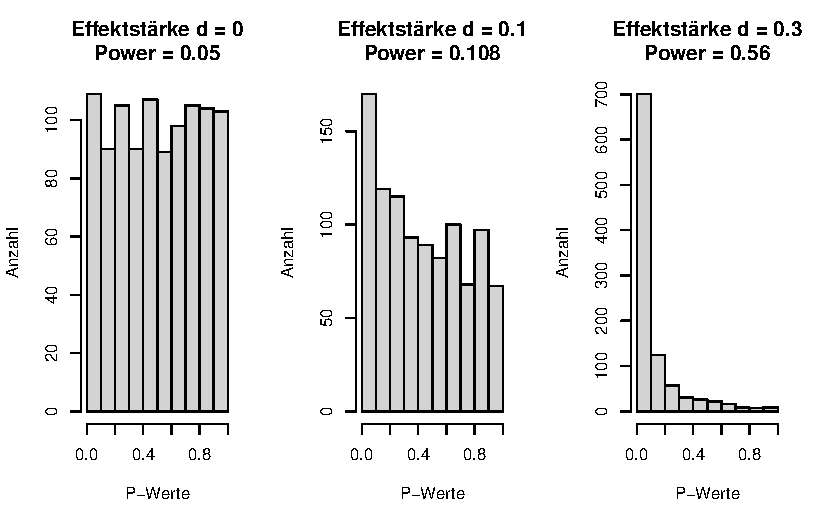
\includegraphics{probleme_methoden_files/figure-pdf/unnamed-chunk-1-1.pdf}

\subsection{\texorpdfstring{Darstellung kalibrierter Modelle als
geplante Modelle
(\emph{Overfitting})}{Darstellung kalibrierter Modelle als geplante Modelle (Overfitting)}}\label{darstellung-kalibrierter-modelle-als-geplante-modelle-overfitting}

Komplexe statistische Modelle haben viele Stellschrauben. Es ist
möglich, die unzähligen Entscheidungen vor Anwendung eines Modells auf
Daten zu treffen, für gewöhnlich werden aber andere Kalibrationen
ausprobiert und eine andere als die geplante hat eine bessere Passung.
Damit ist gemeint, dass beispielsweise bestimmte Variablen mit in ein
Modell aufgenommen werden, um die Vorhersagekraft zu maximieren. Zu
vielen Modellen gehören sogar verschiedene Algorithmen, die auf Basis
festgelegter Regeln entscheiden, wie das Modell aussehen soll. Ein
Modell wird also an ein Datenmuster angepasst. Wird das Vorgehen
transparent offengelegt, ist das absolut in Ordnung. Problematisch wird
es, wenn das beste gefundene Modell als geplantes Modell dargestellt
wird. Das in den Daten vorliegende Muster beinhaltet in
sozialwissenschaftlichen Untersuchungen nämlich fast immer auch ein
Rauschen, also Schwankungen, die auf Messungenauigkeiten oder andere
unbekannte Einflüsse zurückzuführen sind. Diese Einflüsse schwanken
definitionsgemäß (in der psychologischen Testtheorie ist zum Beispiel
die Rede vom \emph{Error}, einer unsystematischen Schwankung, die sich
bei häufiger Messung herausmittelt). Bei zukünftigen Untersuchen wird
das an die vergangenen Daten und das darin enthaltene Rauschen
angepasste Modell dann notwendigerweise schlechter abschneiden, weil das
Rauschen in den neuen Daten ein anderes ist. Man spricht dann von einem
„überangepassten'' Modell oder Overfitting.

\subsection{\texorpdfstring{Tendenz von Menschen, sich selbst zu
bestätigen (\emph{Confirmation
Bias})}{Tendenz von Menschen, sich selbst zu bestätigen (Confirmation Bias)}}\label{tendenz-von-menschen-sich-selbst-zu-bestuxe4tigen-confirmation-bias}

Ein besonderes Problem wissenschaftlicher Methoden ist der Confirmation
Bias. Das Phänomen ist in der wissenschaftlichen Literatur nicht klar
definiert (REF\hyperref[_msocom_7]{{[}LR7{]}}~), hier meine ich damit
die Tendenz von Menschen (oder in diesem Kontext: Forschenden),
diejenigen Muster zu finden, die sie erwarten. Der Confirmation Bias
basiert auf wissenschaftlichen Befunden (Nickerson, 1998; Oswald \&
Grosjean, 2004), und wurde von den Wissenschaftler*innen auf sie selbst
übertragen (Mynatt et al., 1977; Yu et al., 2014). Diese Gedanken führen
nah an logischen Unsinnigkeiten und Paradoxa entlang, selbstironisch
bemerkt zum Beispiel (Nickerson, 1998) die Möglichkeit, dass alle
Befunde zu Confirmation Biases selbst nur Produkte desselben sein
könnten, was die Existenz des Confirmation Biases dann wieder bestätigen
würde (S. 211). Praktisch besteht die Gefahr, dass Wissenschaftler*innen
nicht Wahrheiten herausfinden, sondern alles so drehen, dass ihre
Vorahnungen bestätigt werden. Ludwik Fleck (1935/2015) geht in seiner
Wissenschaftssoziologie, die die Grundlage für Thomas Kuhns Arbeit zu
wissenschaftlichen Revolutionen (1970/1996) bildet, noch ein paar
Schritte weiter: Er argumentiert für ein Modell des wissenschaftlichen
Fortschritts, bei dem es nicht darum geht, der Wahrheit näher zu kommen,
sondern nach bestem Wissen Probleme vor dem gesellschaftlichen
Hintergrund zu verstehen. Das heißt nicht, dass es keine Wahrheit gibt,
nur dass Wahrheit eben nicht bloß die Übereinstimmung von Aussagen mit
Tatsachen ist. Statt dieser oft von Wissenschaftler*innen vertretenen
\emph{Korrespondenztheorie von Wahrheit}, findet sich bei Fleck eine
\emph{Konsenstheorie} von Wahrheit wieder: Die Übereinstimmung vieler
Leute ist wichtig. Wissenschaftliche Tatsachen werden nicht von
einzelnen Personen „entdeckt'', sondern von einem Kollektiv erschaffen.
Der Confirmation Bias findet sich dabei so wieder, dass dem Konsens
widersprechende Befunde ausgeblendet werden und auf den aktuellen
Auffassungen so lange wie möglich beharrt wird. Wenngleich
philosophische Wahrheitstheorien den Rahmen dieses Buches sprengen, sei
darauf hingewiesen, dass keine der drei Wahrheitstheorien
(Korrespondenz, Konsens, und Kohärenz) haltbar ist (Albert, 2010;
\emph{Münchhausen Trilemma}).

\subsection{Datenfälschung}\label{datenfuxe4lschung}

Die bisher diskutierten Praktiken werden oft als fragwürdig
(questionable) dargestellt. Manche Wissenschaftler*innen halten das für
ein Euphemismus, denn in der Verantwortung als Forscher*in sollte
genügend Wissen vorliegen, um zu erkennen, dass die oben beschriebenen
Techniken \emph{nicht} wissenschaftlich sind und eindeutig nicht der
Generierung von Wissen dienen. Sie behindern deutlich den
wissenschaftlichen Fortschritt, gefährden das Vertrauen in Wissenschaft,
und führen zu enorm hohen Kosten. Unglücklicherweise sind diese
Problematiken vielen Wissenschaftler*innen heute immer noch nicht
bekannt. „Das haben wir halt so gelernt und schon immer so gemacht''
heißt es zum Beispiel. Dass bestimmte Studien sich nicht replizieren
ließen, war teilweise schon vielen Personen bewusst, sie hielten es nur
nicht für möglich, das im Scientific Record festzuhalten (z.B.
\url{http://daniellakens.blogspot.com/2020/11/why-i-care-about-replication-studies.html}).
Jedenfalls legt der Begriff der fragwürdigen Forschungspraktiken nahe,
dass sich Forschende damit in einer Grauzone bewegen würden. Meiner
Ansicht nach, ist das nur der Fall, da, wenn Forschende ihren Job
verlieren würden, weil sie P-Hacking betrieben haben, nicht mehr viele
Forschende übrig wären.

Anders ist es beim Fälschen und Manipulieren von Daten. Wie häufig
Datenmanipulationen oder -fälschungen vorkommen ist ungewiss und
Schätzungen sind schwierig. In einer Meta-Analyse von Umfragen zu dem
Thema wurde geschätzt, dass zwischen 0,86 und 4,45\% aller
Wissenschaftler*innen zugaben, Daten manipuliert zu haben. 72\% gaben
an, fragwürdige Forschungspraktiken anzuwenden (Fanelli, 2009). Stroebe
et al.~(2012) stellten später Beispiele von Datenfälschung
\hyperref[_msocom_8]{{[}LR8{]}}~zusammen und empfahlen Peer Review und
Replikationen als Betrugs-Detektoren. Eine neuere und extrem
umfangreiche Studie von Gopalakrishna et al.~(2021) berichtete, dass
8,3\% aller Befragten Daten manipuliert oder gefälscht hätten und 51,3\%
fragwürdige Forschungspraktiken angewandt hätten (Tabelle 2) und
bestätigte den Ausmaß der Probleme. Je nach Disziplinen kommen weitere
Probleme hinzu, wie zum Beispiel die Verwendung bereits veröffentlichter
biomedizinischer Bilder, die in ungefähr 3,8\% aller veröffentlichten
Artikel angewandt wurde (Bik et al., 2016). Es wird davon ausgegangen,
dass Datenfälschung nur in sehr seltenen Fällen aufgedeckt wird.
Diejenigen Fälle, die ans Licht kamen, hatten die Zurückziehung
(\emph{Retraction}) der jeweiligen wissenschaftlichen Artikel zur Folge
und oft Konsequenzen für die wissenschaftliche Karriere der
Verantwortlichen. Retractionwatch.org verwaltet die weltweit größte
Datenbank zu zurückgezogenen Artikeln (Stand Dezember 2023: 49.628
Artikel): \url{http://retractiondatabase.org/}.

Sehr düster ist dabei die Tatsache, dass Methoden zur Datenfälschung
einerseits immer einfacher werden (e.g., Naddaf,
2023)\hyperref[_ftn1]{{[}1{]}} und Wissenschaftler*innen, die Fehler
aufdecken, häufig verklagt werden. Das betrifft beispielsweise wurden
die Autoren von Datacolada.org, die bereits häufiger Probleme aufgezeigt
haben, von Francesca Gino für die Veröffentlichung verklagt
(\url{https://datacolada.org/109}), woraufhin tausende
Wissenschaftler*innen Gelder für die finanzielle Unterstützung des
Gerichtsprozesses sammelten
(\url{https://www.gofundme.com/f/uhbka-support-data-coladas-legal-defense}).

\hyperref[_ftnref1]{{[}1{]}} Hussey
(\url{https://osf.io/preprints/psyarxiv/4kht8}) und Sarstedt \& Adler
(\url{https://www.sciencedirect.com/science/article/abs/pii/S0148296323003004})
haben sarkastisch Methoden vorgeschlagen, direkt die berichteten Werte
automatisiert fälschen zu lassen.

~\hyperref[_msoanchor_1]{{[}LR1{]}}\url{https://www.thelancet.com/journals/lancet/article/PIIS0140-6736(14)60932-6/fulltext?version\%3DprinterFriendly=&code=lancet-site}

hier müssten statistiken sein

~\hyperref[_msoanchor_2]{{[}LR2{]}}Hier beta-fehler erklären und power

~\hyperref[_msoanchor_3]{{[}LR3{]}}Wicherts liste:
https://www.ncbi.nlm.nih.gov/pmc/articles/PMC5122713/

~\hyperref[_msoanchor_4]{{[}LR4{]}}Abbildung passt nicht ganz zum
Beispiel

~\hyperref[_msoanchor_5]{{[}LR5{]}}\url{http://dx.doi.org/10.1111/jpim.12738}

~\hyperref[_msoanchor_6]{{[}LR6{]}}binom.test(1, 3, .05)

~\hyperref[_msoanchor_7]{{[}LR7{]}}abschlussarbeit confirmation bias
samira nickel

~\hyperref[_msoanchor_8]{{[}LR8{]}}Podcast zu dem Thema:

\url{https://freakonomics.com/podcast/can-academic-fraud-be-stopped/}

\subsection{Literatur}\label{literatur-8}

\chapter{Theorien}\label{theorien}

Wissenschaft \hyperref[_msocom_1]{{[}LR1{]}}~arbeitet mit Theorien. Wie
diese genau aussehen, unterscheidet sich zwischen Disziplinen massiv.
Während naturwissenschaftliche Bereiche häufig mit mathematischen
Modellen, also Formeln, arbeiten, die den Zusammenhang zwischen
Variablen explizit und unmissverständlich beschreiben und Vorhersagen
erlauben, arbeiten Sozialwissenschaften häufig mit verbalen Theorien im
Stile von „X und Y hängen positiv miteinander zusammen'' oder „je höher
X, desto höher Y'' und traditionelle Geisteswissenschaften arbeiten
beispielsweise mit verbalen Erklärungen. Verbale Theorien haben den
Vorteil, dass sie tendenziell leicht verständlich und allgemein
anwendbar sind, allerdings unterliegen die verwendeten Begriffe häufig
individuellen, kulturellen, oder zeitlichen Einflüssen und
Diskutant*innen droht, im wissenschaftlichen Diskurs aneinander vorbei
zu reden. Für formale Theorien werden alle beteiligten Variablen genau
definiert und die Theorien haben häufig einen stark eingeschränkten
Geltungsbereich (z.B. gelten viele physikalische Gesetze nur unter
streng kontrollierten Bedingungen wie im Vakuum, bei einer bestimmten
Temperatur, usw.). Die Sorge im Rahmen der Replikationskrise ist, dass
Theorien nicht klar genug sind, um vorherzusagen, wann Replikationen
erfolgreich sind und damit eine der Ursachen für geringe
Replikationsraten sind (z.B. REF\hyperref[_msocom_2]{{[}LR2{]}}~). Eine
Theorie über die Konsequenzen von der Identifikation mit
Geschlechterrollen muss beispielsweise die Veränderung von
Geschlechterrollen und Besonderheiten von Geschlechterrollen in
verschiedenen Ländern berücksichtigen. Dass ein und dasselbe Experiment
zu diesem Thema in den USA im Jahre 1980 andere Ergebnisse hat als in
Deutschland im Jahr 2020 ist wenig überraschend. Problematisch ist
allerdings, dass -- auch wenn solche Ergänzungen für viele
sozialwissenschaftliche Theorien sinnvoll und nötig erscheinen -- nur
selten Aussagen darüber gemacht werden.

Verbale Theorien sind per se nicht weniger wissenschaftlich. Im Kontext
der jeweiligen Bereiche heben sich wissenschaftliche Theorien stets
durch ihren besonders hohen Grad an Systematizität (Hoyningen-Huene,
2013) von alltagswissenschaftlichen Erklärungen ab. Bereiche, die Wert
auf Vorhersage von Geschehnissen legen, kommen jedoch nicht ohne formale
Theorien aus (Muthukrishna \& Henrich, 2019). Dabei sei hervorgehoben,
dass bestimmte Wissenschaften eben \emph{keinen Wert} auf Vorhersage
legen (z.B. Geschichtswissenschaften oder Disziplinen, die vorwiegend
hermeneutisch vorgehen). Sozialwissenschaften wie die Psychologie,
quantitative Soziologie, oder Teile der Geisteswissenschaften („Digital
Humanities'') nähern sich aktuell formalen Modellen an -- in der
Sozialpsychologie gab es den Aufruf, Theorien zu formalisieren
beispielsweise schon einmal bei einer Krise in den 1970er Jahren
(Lakens, 2023). Dadurch, dass sich Theorien durch ihren Mangel an
Objektivität selten von verschiedenen Forschenden verwendet werden und
sich durch ihre flexible Auslegung nur schwer wiederlegen lassen ist
dort eine enorm große Menge an nutzlosen Theorien entstanden (Ferguson
\& Heene, 2012). Darunter sind auch einander widersprechende Theorien:
Beispielsweise argumentieren Banker et al.~(2017), dass „ego
depletion'', also die Erschöpfung von Selbstkontrollressourcen, dazu
führt, dass Personen sich eher an Hinweise anderer Leute orientieren (S.
2) während Francis et al.~(2018) gegenteilig vermuten, dass die
Erschöpfung verhindert, dass Hinweise überhaupt verarbeitet werden
können. Beide lieferten Daten, die die jeweiligen Theorien bestätigten,
jedoch fand eine Folgeuntersuchung, dass vermutlich beide falsch lagen
(Röseler et al., 2020).

Robinaugh et al.~(2021) diskutieren Beispiele der Umwandlung verbaler
Theorien in formale. Dieser Prozess hat zur Folge, dass sich neue und
spezifischere Vorhersagen ableiten lassen. Wenn eine Theorie genauere
Vorhersagen macht und die Menge an möglichen Ereignissen, die der
Theorie widersprechen, steigt, bedeutet das einen gestiegenen
\emph{empirischen Gehalt} (siehe Tabelle Z; Glöckner \& Betsch, 2011;
Popper, 1959/2008).

\textbf{TABELLE Z}

\emph{Aussagen über den Zusammenhang von X und Y mit verschiedenen
Graden an empirischem Gehalt}\hyperref[_msocom_3]{{[}LR3{]}}~

XXX

\subsection{\texorpdfstring{Deduktion und
\hyperref[_msocom_4]{{[}LR4{]}}~Induktion}{Deduktion und {[}LR4{]}~Induktion}}\label{deduktion-und-lr4-induktion}

Methoden werden reformiert und Wissenschaftler*innen diskutieren, wie
Wissenschaft funktioniert, ablaufen sollte, und welche Methoden sinnvoll
und unsinnig sind. Wie am hermeneutischen Zirkel klar wird, führt ein
Erkenntnisweg darüber, eine Menge von Beobachtungen zu einer
Regelmäßigkeit oder Gesetzmäßigkeit zusammenzufassen (\emph{Induktion})
und ein weiterer besteht daraus, aus einer Gesetzmäßigkeit bzw. Theorie
Vorhersagen über noch nicht angestellte Beobachtungen zu machen
(\emph{Deduktion}). Immer wieder wird diese Unterscheidung im
wissenschaftlichen Diskurs vernachlässigt oder ausgeblendet.
Beispielsweise drehte sich ein Dialog in der Konsumentenpsychologie
jahrelang darum, welcher Weg besser sei, obwohl beide Wege gleichermaßen
legitim sind und einander ergänzen (e.g., Calder et al., 1981). Ähnlich
verhält es sich bei Konflikten zwischen qualitativer und quantitativer
Vorgehensweise, die formal betrachtet jeweils eher induktiv oder
deduktiv vorgehen (Borgstede \& Scholz, 2021). Bei Replikationsforschung
hat traditionell die induktive Seite mehr Beachtung erfahren (Hüffmeier
et al., 2016): Jeder Unterschied zwischen Replikation- und
Originalstudie wird als mögliche Ursache für ein Scheitern des
Replikationsversuches herangezogen um die Vertrauenswürdigkeit der
Originalbefunde aufrechtzuerhalten (Baumeister \& Vohs, 2016). Dabei
gerät außer Acht, dass kleinere Unterschiede zwischen Original- und
Replikationsstudie (z.B. Verwendung der Maße, durchschnittliches Alter
der Versuchspersonen, Sprache der Instruktion) von Theorien nicht
erfasst werden -- ihnen zufolge also unerheblich sein sollten -- und
eine fehlgeschlagene Replikation klar die Grenzen der Theorie aufzeigt
und sich aus ihr Empfehlungen für die Modifikation von Theorien ableiten
lassen (Cesario, 2014; Dijksterhuis, 2014). Ein Überblick über die
Vorgehensweisen ist in Tabelle X.

\textbf{Tabelle X}

\emph{Merkmale induktiver u}\hyperref[_msocom_5]{{[}LR5{]}}~\emph{nd
deduktiver Vorgehensweise}

\begin{longtable}[]{@{}
  >{\raggedright\arraybackslash}p{(\columnwidth - 12\tabcolsep) * \real{0.0158}}
  >{\raggedright\arraybackslash}p{(\columnwidth - 12\tabcolsep) * \real{0.1234}}
  >{\raggedright\arraybackslash}p{(\columnwidth - 12\tabcolsep) * \real{0.0158}}
  >{\raggedright\arraybackslash}p{(\columnwidth - 12\tabcolsep) * \real{0.3639}}
  >{\raggedright\arraybackslash}p{(\columnwidth - 12\tabcolsep) * \real{0.0158}}
  >{\raggedright\arraybackslash}p{(\columnwidth - 12\tabcolsep) * \real{0.4494}}
  >{\raggedright\arraybackslash}p{(\columnwidth - 12\tabcolsep) * \real{0.0158}}@{}}
\toprule\noalign{}
\endhead
\bottomrule\noalign{}
\endlastfoot
& & & & & & \\
& \textbf{Facette} & & \textbf{Deduktives Vorgehen (Theorie-geleitet)} &
& \textbf{Induktives Vorgehen (Phänomen-geleitet)} & \\
& & & & & & \\
& Verallgemeinerbarkeit steckt in\ldots{} & & der Theorie: Sie ist a
priori maximal allgemein (z.B. gilt sie, bis anderweitig nachgewiesen,
für alle Menschen). & & den Daten: Erst vielfältige Beobachtungen in
verschiedenen Kontexten erlauben die Annahme, dass das Phänomen
allgemeingültig ist. & \\
& & & & & & \\
& Veränderung von Verallgemeinerbarkeit & & Mit mehr Beobachtungen sinkt
die Allgemeingültigkeit. & & Mit mehr Beobachtungen steigt die
Allgemeingültigkeit (sofern sie bestätigender Natur sind). & \\
& & & & & & \\
& Art der Prüfung & & Vorhersagen der Theorie werden vorwiegend
Versuchen der \emph{Widerlegung} unterzogen. & & Wiederholte
Beobachtungen \emph{bestätigen} den ursprünglichen Einzelfall. & \\
& & & & & & \\
& Wahl des Studiensettings & & Studentische Stichproben aus nur einem
Land oder Laboruntersuchungen sind unbedenklich. & & Der Kontext der
Untersuchung sollte die Zielbedingungen (z.B. bei der Anwendung der
Erkenntnisse in der Praxis) möglichst gut widerspiegeln. & \\
& & & & & & \\
\end{longtable}

\subsection{Hilfshypothesen}\label{hilfshypothesen}

Über folgende Wege lassen sich Replikationsfehlschläge erklären:

1.~~~~~ Fehler erster Art der Originalstudie: Der Originalbefund war nur
ein Zufallsbefund oder kam durch wissenschaftliches Fehlverhalten
zustande (siehe Kapitel „Freiheitsgrade von Forschenden (Researchers'
Degrees of Freedom)``).

2.~~~~~ Fehler erster Art der Replikationsstudie: Die Originalstudie lag
richtig, die Replikationsstudie hat einen Fehler gemacht (z.B. zu kleine
Stichprobe, schlechte Kalibrierung der Instrumente, oder
wissenschaftliches Fehlverhalten).

3.~~~~~ Grenzbereich des Phänomens: Beide Studien sind vertrauenswürdig.
Die Replikationsstudie \emph{unterscheidet} sich auf eine für die
Theorie wichtige Weise (z.B. wurde die Replikationsstudie mit Personen
aus einem anderen Land durchgeführt und die Theorie gilt nur für
Menschen aus dem „Original-Land''). Siehe hierzu auch Fanelli
(REF\hyperref[_msocom_6]{{[}LR6{]}}~).

Variante 3 ist konstruktiv und nimmt beide Einzelbefunde für robust hin.
Notwendig dafür ist ein theoretisch relevanter Unterschied zwischen der
Original- und Replikationsstudie, der durch die unendliche Anzahl
möglicher wichtiger Faktoren in den meisten Fällen zutrifft (Smedslund,
2015). Über diesen Weg lässt sich die Theorie dann modifizieren oder
eine weitere Theorie aufstellen, die für den Kontext der Untersuchung
ebenfalls berücksichtigt werden muss.

~\hyperref[_msoanchor_1]{{[}LR1{]}}einarbeiten:
\url{https://link.springer.com/article/10.1007/s43638-023-00081-3}

•~~~~~~ \url{https://doi.org/10.31234/osf.io/jqw35}

•~~~~~~ Smaldino, P. (2019). Better methods can't make up for mediocre
theory. \emph{Nature}, \emph{575}(7781), 9.
https://doi.org/10.1038/d41586-019-03350-5

•~~~~~~ ~

~\hyperref[_msoanchor_2]{{[}LR2{]}}\url{https://journal.trialanderror.org/pub/tension-between-theory/release/1}

~\hyperref[_msoanchor_3]{{[}LR3{]}}Siehe ppt folien von meinem seminar

~\hyperref[_msoanchor_4]{{[}LR4{]}}Validitätsarten in Call for
Replications in Language Teaching:
\url{https://www.sciencedirect.com/science/article/pii/S2772766123000514}

Viel external und internal validity

~\hyperref[_msoanchor_5]{{[}LR5{]}}Aus preprint mit Johannes genommen,
evtl anpassen oder zitieren

~\hyperref[_msoanchor_6]{{[}LR6{]}}12:15
\url{https://www.youtube.com/watch?v=CEAV7420jBk}

\subsection{Literatur}\label{literatur-9}

\chapter{Epistemische Probleme}\label{epistemische-probleme}

Möglichkeiten der Epistemologie, also der Erkenntnislehre,
Replikationsprobleme zu erklären, übersteigen systemische und
methodische Faktoren, haben aber auch andere Prüfbarkeitsansprüche und
sind für tätige Wissenschaftler*innen wahrscheinlich eher unplausibel.

\subsection{Komplexität von Studien}\label{komplexituxe4t-von-studien}

\url{https://osf.io/preprints/metaarxiv/5r36g} siehe auch Fanellie talk
\url{https://www.youtube.com/watch?v=CEAV7420jBk} und evtl. gibt es
inzwischen prereg Test von ihm

\subsection{\texorpdfstring{Robustheit und Historizität von
\hyperref[_msocom_1]{{[}LR1{]}}~Phänomenen\hyperref[_msocom_2]{{[}LR2{]}}~}{Robustheit und Historizität von {[}LR1{]}~Phänomenen{[}LR2{]}~}}\label{robustheit-und-historizituxe4t-von-lr1-phuxe4nomenenlr2}

Unter welchen Voraussetzungen ist es wenig überraschend, dass
Replikationsversuche fehlschlagen? Ein Ausweg ist anzunehmen, dass die
untersuchten Phänomene extrem empfindlich oder unstabil seien.
Regelmäßigkeiten im menschlichen Verhalten analog zu den
Planetenbewegungen zu entdecken könnte schlichtweg nicht möglich sein
(Smedslund, 2015). Weniger extreme Annahmen über die Existenz von
Regelmäßigkeiten, die möglicherweise nicht jede Person ausnahmslos
betreffen aber „im Schnitt'' gelten (also aristotelische statt
galileische Gesetzmäßigkeiten; Lewin, 1930) sind allerdings
unumstritten. Eine solche Regelmäßigkeit kann zum Beispiel sein, dass
Männer größer als Frauen sind. Noch extremer ist die Theorie, dass
Menschen sich des Wissens über sie bewusst sind und ihr Verhalten
dynamisch anpassen und Verhaltenswissenschaften immer historisch bzw.
zeitgebunden sind: Wird herausgefunden, dass Menschen in ihren
Entscheidungen tendenziell dazu neigen nichts zu ändern, auch wenn sich
dadurch ihre Situation verbessern würde, wird ihnen diese Tatsache über
die Wissenschaft vor Augen geführt und sie können ihr Verhalten
anpassen. Dabei handelt es sich übrigens um den Status Quo Bias, welcher
im Rahmen von über 30 Jahren erfolgreich repliziert wurde (Samuelson \&
Zeckhauser, 1988; Xiao et al., 2021).

Wie stark sich Phänomene durch vermeintlich kleinere Unterschiede im
Versuchsaufbau unterscheiden wurde bereits meta-wissenschaftlich
untersucht. Landy et al.~(2020) ließen mehrere Hypothesen von mehreren
Forschenden prüfen und Faktoren, die laut den dahinterliegenden Theorien
eigentlich keinen Unterschied machen sollten, führten dazu, dass
Gegenteilige Ergebnisse entstanden. Auf Replikationsforschung übertragen
ist es also möglich, dass in bestimmten Forschungsbereichen völlig
unklar ist, unter welchen Bedingungen welche Zusammenhänge zu beobachten
sind.

\subsection{Paradox des Fallibilität und des
Fortschritts}\label{paradox-des-fallibilituxe4t-und-des-fortschritts}

-~~~~~~~~~ \url{https://www.pnas.org/doi/full/10.1073/pnas.1711786114}
{[}einarbeiten{]}

~\hyperref[_msoanchor_1]{{[}LR1{]}}Error is an integral part of the
process of science

\url{https://www.pnas.org/doi/full/10.1073/pnas.1711786114}

~\hyperref[_msoanchor_2]{{[}LR2{]}}in BA Literaturverzeichnis schauen
why psych cannot be a science

\subsection{Literatur}\label{literatur-10}

\part{Lösungen}

\part{Lösungen und Ansätze zur Verbesserung der Lage der Psychologie}

Werfen wir ein Blick darauf, was sich seit 2012 in der Psychologie
verändert hat. Eingeteilt sind die Veränderungen dahingehend, welchen
Teil des Problems sie vor allem betreffen: Ist der Zweck einer neuen
Vorgabe, das System, die Methodik, oder die Theorien der Forschung zu
verbessern? Einige Lösungen sind mit vielen Problemen gleichzeitig
verknüpft und manche sind auf bestimmte Angelegenheiten maßgeschneidert.
Abbildung 3 enthält eine grobe Unterteilung.

\begin{figure}[H]

{\centering 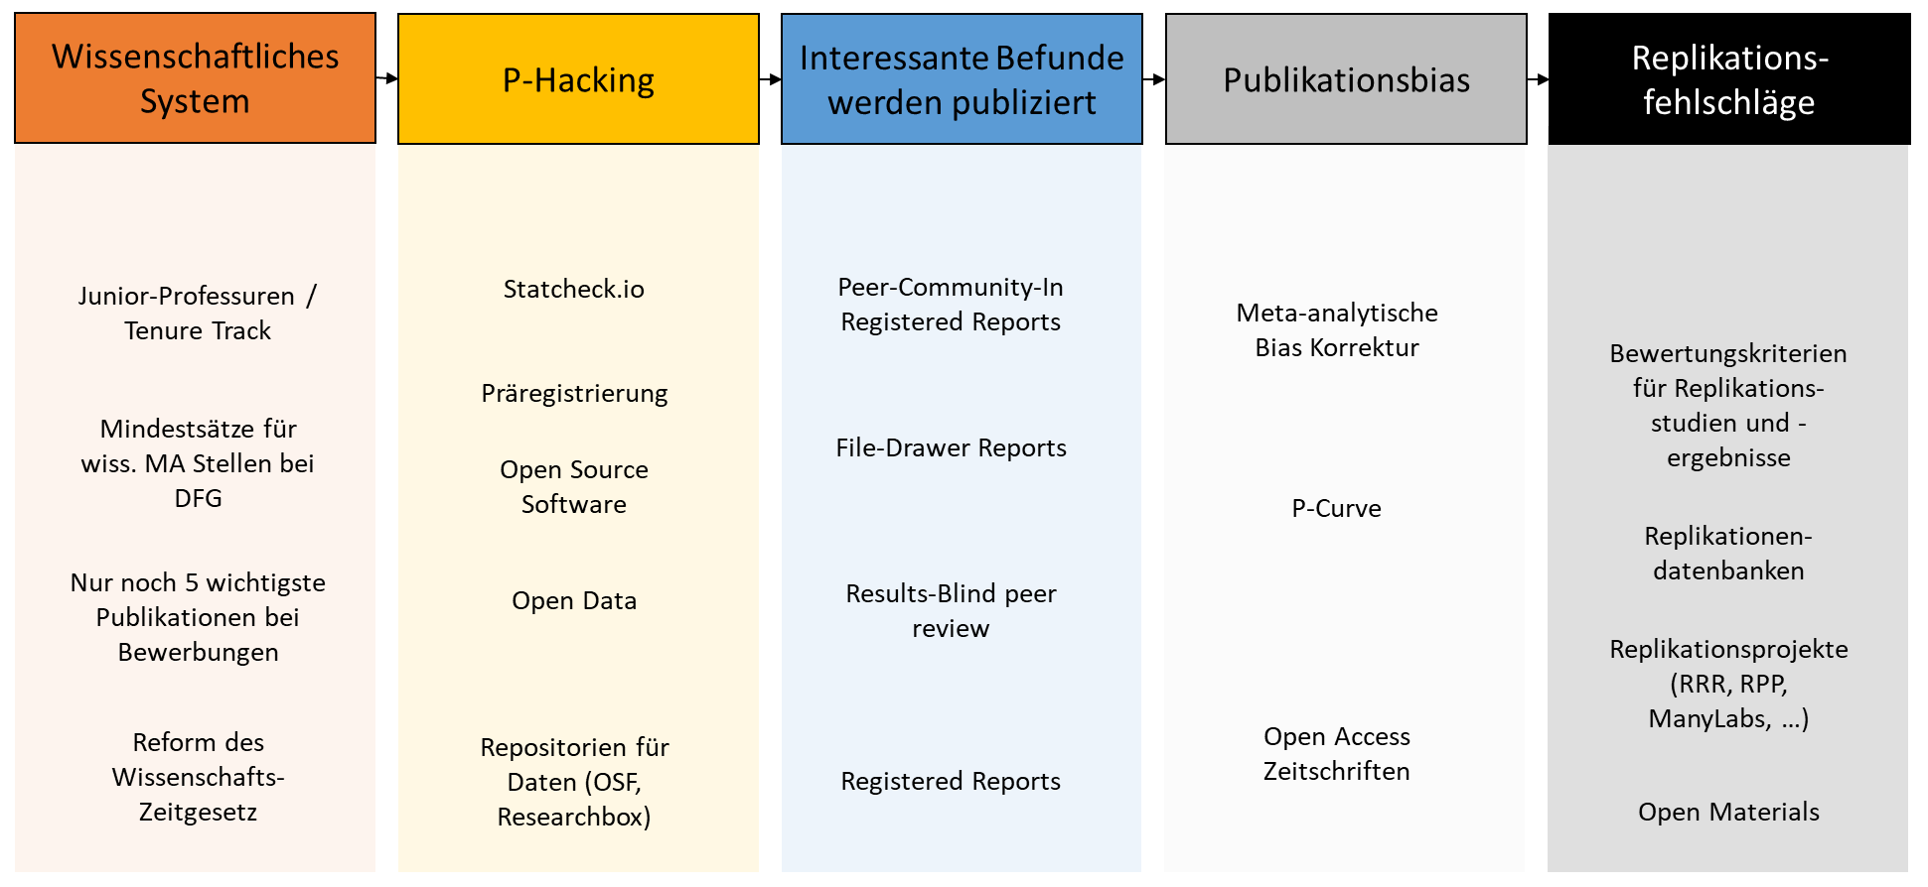
\includegraphics{images/lösungsansätze.png}

}

\caption{Lösungsansätze und welches Problem in der Wissenschaft sie
aufgreifen}

\end{figure}%

\section*{}\label{section}
\addcontentsline{toc}{section}{}

\markright{}

\chapter{Das System}\label{das-system}

Fangen wir mit dem System an. Ich selbst verspreche mir von diesen
Ansätzen am meisten, denn solange Publikationen die Währung sind und
Paper mit knackigen Titeln und eindeutigen Ergebnissen als qualitativ
hochwertiger befunden werden, sind Forschende darin motiviert, statt der
Wahrheit eben nach knackigen Titeln und eindeutigen Ergebnissen zu
suchen.

Allgemein ist eine positive Entwicklung sichtbar (REF
\url{https://www.nature.com/articles/s44271-023-00003-2} ) und eine
Veränderung der Anreizstruktur wird anvisiert. Sie lässt sich als
Angleichung des wissenschaftlichen Systems an die \emph{Mertonschen
Normen} (nach Robert Merton) auffassen\hyperref[_msocom_1]{{[}LR1{]}}~:
(1) Kommunismus: Das wissenschaftliche Wissen sollte allen
Wissenschaftler*innen gleichermaßen gehören, um die Zusammenarbeit zu
fördern. (2) Universalismus: Wissenschaftliche Güte ist unabhängig vom
soziopolitischen Status und persönlichen Attributen der Teilhabenden.
(3) Desinteresse: Wissenschaftliche Institutionen handeln im Interesse
der Wissenschaft und nicht für persönlichen Gewinn. (4) Organisierter
Skeptizismus: Wissenschaftliche Behauptungen sollten einer kritischen
Prüfung unterzogen werden bevor sie akzeptiert werden.

Nosek (REF, 2019 make it possible, siehe Abbildung X) empfiehlt eine
Maßnahmenstruktur, nach welcher die gewünschten Veränderung nacheinander
\ldots{}

1.~~~~~ möglich\\
(z.B. durch Infrastruktur wie online Repositorien, in denen
Forschungsmaterialien öffentlich und gratis hochgeladen werden können),

2.~~~~~ einfach\\
(z.B. durch barrierearme Angebote, mehrsprachige Anleitungen),

3.~~~~~ normativ\\
(z.B. durch Wissenschaftliche Communities, die gemeinsam hinter
Forderungen der Verbesserung stehen),

4.~~~~~ belohnend\\
(z.B. durch designierte Preise), und

5.~~~~~ notwendig\\
(z.B. durch Mindeststandards, die von Zeitschriften oder
Drittmittelgebern gefordert werden)

gemacht werden sollen. Wie die verschiedenen Ansätze bei den
verschiedenen Akteuren, also Politik, Universitäten, oder Zeitschriften
konkret aussehen, wird im Folgenden diskutiert.

Abbildung X

\emph{Kulturwandel in der Wissenschaft nach Nosek (2019, Abbildung N,
REF)}

\emph{PYRAMIDE HIER EINFÜGEN AUF DEUTSCH XXX}

\subsection{Infrastruktur (Open
Infrastructure)}\label{infrastruktur-open-infrastructure}

-~~~~~~~~~ ermöglichend

-~~~~~~~~~ NFDI

-~~~~~~~~~ Prinzipien: \url{https://openscholarlyinfrastructure.org}
(übersetzen, einfügen, zitieren)

-~~~~~~~~~ Beispiele

o~~ Wege, um Materialien, Daten, oder Ergebnisse

§~ Literaturdatenbanken (OpenAlex)

§~ (Data) Repositories, re3data.org; OSF.io

§~ Pre-Print Server (arXiv), Zeitschriften, Zeitschriftensysteme (OJS)

§~ Begutachtungssysteme (PCI)

§~ Post-Publication Review

o~~ Meta-Daten, um Verweise zu ermöglichen (ORCID-ID, ROR
\url{https://ror.org}, DOI)

§~ ORCID-ID Kritik:
\url{https://www.sciencedirect.com/science/article/pii/S0099133324000144?dgcid=rss_sd_all}

-~~~~~~~~~ Übersicht:
\url{https://kumu.io/access2perspectives/open-science\#disciplines/by-os-principle/open-infrastructure?focus=1}
von
\url{https://access2perspectives.org/mapping-open-science-resources/}

\subsection{Politik}\label{politik}

International stehen politische Parteien und Vereinigungen deutlich
hinter Open Science und Open Access. Beispielsweise empfiehlt die UNESCO
einen universellen Zugang zu wissenschaftlichen Wissen ungeachtet von
Herkunftsland, Geschlechterrolle, politischen Grenzen, Ethnizität, oder
ökonomischen oder technologischen Hürden (REF
\url{https://unesdoc.unesco.org/ark:/48223/pf0000374837}, p.~3).
Arbeitsgruppen für politische Instrumente, Förderung, und Infrastruktur
wurden entsprechend gegründet (REF\hyperref[_msocom_2]{{[}LR2{]}}~). Die
G7 setzen sich für wissenschaftliche Integrität, akademische Freiheit,
und Open Science ein (REF\hyperref[_msocom_3]{{[}LR3{]}}~). Offener
Zugang (REF\hyperref[_msocom_4]{{[}LR4{]}}~) aber auch Transparenz des
wissenschaftlichen Vorgehens (REF\hyperref[_msocom_5]{{[}LR5{]}}~) wird
auch seitens der Europäischen Union gefordert. Infrastruktur (z.B.
European Open Science Cloud, https://eosc-portal.eu) und diverse Open
Science Forschungsprojekte werden gefördert.

In Deutschland hat sich die Regierung des Zyklus 2021-2025 im Rahmen des
Koalitionsvertrages vorgenommen, „Open Access \ldots{} als gemeinsamen
Standard {[}zu{]} etablieren.'' Einzelne Bundesländer wie
Nordrhein-Westfalen haben in Zusammenschlüssen aus den jeweiligen
Universitäten darüber hinaus Open Access Strategien entwickelt
(REF\hyperref[_msocom_6]{{[}LR6{]}}~) und arbeiten aktuell an Open
Science Strategien. Andere Länder, wie zum Beispiel Schweden, haben
bereits nationale Richtlinien zu Open Science entwickelt
(\url{https://www.kb.se/samverkan-och-utveckling/nytt-fran-kb/nyheter-samverkan-och-utveckling/2024-01-15-national-guidelines-for-promoting-open-science-in-sweden.html}).
Hinsichtlich der Problematik von Machtmissbrauch wird das Problem
beispielsweise in einem Eckpunkte-Papier des Landes NRW anerkannt, doch
als Einzelfall- statt System-Problem verstanden
(REF\hyperref[_msocom_7]{{[}LR7{]}}~, für einen Kommentar siehe z.B.
REF\hyperref[_msocom_8]{{[}LR8{]}}~).

\subsection{\texorpdfstring{Universitäten\hyperref[_msocom_9]{{[}LR9{]}}~}{Universitäten{[}LR9{]}~}}\label{universituxe4tenlr9}

Das Thema Open Science hat bei vielen Universitäten bereits Anklang
gefunden. Während die meisten deutschen Universitäten Mittel für Open
Access Publikationen haben, existieren an einigen darüber hinaus Open
Science Policys (z.B. FAU Erlangen,
\url{https://oa-info.sh/2022/01/open-science-policy-der-uni-erlangen-nuernberg/}),
Open Science Centers (z.B.
\href{https://www.osc.uni-muenchen.de/index.html}{LMU Open Science
Center}, \url{https://osf.io/smqpn}; Köln Open Science Center; Münster
Center for Open Science;
\href{https://www.uni-mannheim.de/open-science/open-science-office/}{Mannheim
Open Science Office}). Darüber hinaus unterstützen das
Leibniz-Informationszentrum Wirtschaft in Kiel und das Leibniz-Institut
für Psychologie Replikationsforschung beispielsweise mit einer
Replikationszeitschrift (\url{https://www.jcr-econ.org}) oder im Rahmen
einer Juniorprofessur für Psychologische Metawissenschaft. Eines der
Metawissenschaftlichen Zentren innerhalb Europas hat sich in den
Niederlanden in Tilburg gebildet. Die Berliner Universitäten haben eine
gemeinsame Open Access Erklärung entwickelt
(\url{https://openaccess.mpg.de/Berliner-Erklaerung}\hyperref[_msocom_10]{{[}LR10{]}}~)
und in Frankreich ist die Universität Sorbonne ein Pionier: Gemeinsam
mit der Universität Amsterdam und dem Universitätscollege London wurde
eine Erklärung über die die Veröffentlichung von Forschungsdaten
unterzeichnet. XXX\hyperref[_msocom_11]{{[}LR11{]}}~. Seit 2024 hat die
Universität Sorbonne darüber hinaus den Vertrag mit Clarivate für die
Nutzung der Forschungsdatenbank „Web of Science'' gekündigt und arbeitet
seitdem mit der Open Source Software „OpenAlex''
(REF\hyperref[_msocom_12]{{[}LR12{]}}~).

Für die langfristige Entwicklung der Wissenschaften haben Universitäten
dadurch eine besondere Verantwortung, dass sie Wissenschaftler*innen
beschäftigen und an ihnen die Auswahl für die wenigen unbefristeten
Arbeitsplätze in der Wissenschaft fallen. Wenn jahrzehntelang
Professuren auf Basis subjektiver, nicht-reproduzierbarer, und für gute
Wissenschaft nachrangigen Kriterien gewählt werden (z.B. Anzahl an
Publikationen in Fachzeitschriften), kann sich das negativ auf die
Entwicklung von Wissenschaften auswirken. Ein Forschungspreis des Berlin
Institute of Health (BIH), der jährlich für Projekte zur Förderung von
wissenschaftlicher Integrität verliehen wird, ging 2023 an ein Projekt,
das objektive und sinnvolle Auswahlkriterien für Professor*innen
entwickelt (REF, REF\hyperref[_msocom_13]{{[}LR13{]}}~). Innerhalb von
Universitäten spielen außerdem die Bibliotheken eine aufklärerische
Rolle hinsichtlich Forschungsdatenmanagement und Publikationskultur
(REF, \url{https://liberquarterly.eu/article/view/14947}). Über sie kann
der Forschungsprozess mit entsprechender Infrastruktur (z.B. zum Lagern
und Veröffentlichen von Forschungsmaterialien und -ergebnissen)
unterstützt werden (z.B. REF\hyperref[_msocom_14]{{[}LR14{]}}~) und
verhindert werden, dass sich eine „Abhängigkeit von wenigen
kommerziellen Anbietern'' ergibt, die „begrenzen, was {[}be{]} der
Forschung an Arbeitsmöglichkeiten und Fragestellungen erreichbar ist''
(REF\hyperref[_msocom_15]{{[}LR15{]}}~). Eine Pflicht, Mitglieder eine
Universität zur Einhaltung von Open Science Strategien zu bewegen, haben
Universitäten jedoch nur eingeschränkt durch den hohen Stellenwert der
„Freiheit der Forschung'' sowie der Gefahr, für Forschende weniger
attraktiv zu werden, wenn beispielsweise auf namhafte Zeitschriften
nicht mehr über die Universität zugegriffen werden kann, weil Verträge
mit closed-access Zeitschriften gekündigt wurden. Beispielsweise klagte
die juristische Fakultät der Universität Konstanz gegen eine
Zweitveröffentlichungspflicht (REF\hyperref[_msocom_16]{{[}LR16{]}}~),
nach welcher Forschende von ihrem Zweitveröffentlichungsrecht Gebrauch
machen müssen oder es werden Zeitschriften, deren wissenschaftliche
Qualität angezweifelt wird, dennoch mit Mitteln zur Veröffentlichung
bezuschusst
(\url{https://www.suub.uni-bremen.de/ueber-uns/neues-aus-der-suub/unter-kritischer-beobachtung-open-access-publikationen-im-mdpi-verlag}).

Eine oft vernachlässigte Rolle kommt außerdem der universitären Lehre
hinzu. Durch die Freiheit von Forschung und Lehre und bereits
durchgeplanten Studiengängen gestaltet sich die Integration von Open
Science in die Lehre schwierig. Forschende, in deren Lehre die Thematik
eine Rolle spielt, teilen proaktiv ihre Materialien, erstellen gemeinsam
Curricula, und sind beispielsweise in großen internationalen Initiativen
wie dem Framework for Open and Reproducible Research Training
(FORRT.org) vernetzt (konkrete Vorschläge zur Integration von Open
Science in die Lehre siehe z.B. REF\hyperref[_msocom_17]{{[}LR17{]}}~).

\subsection{Institute und
Vereinigungen}\label{institute-und-vereinigungen}

Wissenschaftliche Gebiete leben vor allem durch Communities, also alle
in dem Bereich forschenden Personen. Sie organisieren sich üblicherweise
in Vereinen (z.B. Deutsche Gesellschaft für Psychologie),
Interessensverbunden, oder ähnlichen Gemeinschaften. Eine besondere
Stellung hat in Deutschland die Deutsche Forschungsgemeinschaft, welche
staatlich und über die Bundesländer mit mehreren Milliarden Euro
ausgestattet Forschungsgelder vergibt. Als eine der wichtigsten
nationalen Institution hat ihre Open Science Positionierung einen hohen
Stellenwert (REF\hyperref[_msocom_18]{{[}LR18{]}}~), erfahrungsgemäß
gehen Veränderungen jedoch nicht von der DFG aus, sondern die DFG wartet
auf Anstöße aus den Fächern. DGPs\hyperref[_msocom_19]{{[}LR19{]}}~. In
der Psychologie fördert darüber hinaus das ZPID die Infrastruktur durch
Zeitschriften, Pre-Print Server, und weitere Methoden
(REF\hyperref[_msocom_20]{{[}LR20{]}}~). Auch interdisziplinäre
Vereinigungen wie das CERN (REF\hyperref[_msocom_21]{{[}LR21{]}}~) oder
internationale Akteure wie die American Psychological Association
(REF\hyperref[_msocom_22]{{[}LR22{]}}~) verpflichten sich Offenheit und
Transparenz. Für Bürger*innen der Europäischen Union existieren die
European Open Science Cloud und die Open Access Publishing Plattform
\emph{Open Research Europe}.

Im Rahmen der Open Science Reform entstanden außerdem viele neue
Vereinigungen. Das interdisziplinäre und besonders von
Wissenschaftler*innen in der frühen Karrierephase geleitete FORRT
(REF\hyperref[_msocom_23]{{[}LR23{]}}~) setzt sich für eine Verankerung
von Open Science in der Lehre ein. Der Verbesserung psychologischer
Forschung hat sich die Society for the Improvement of Psychological
Science (SIPS) verschrieben. Sogenannte „grassroot''-Initiativen (also
von jungen Wissenschaftler*innen ausgehende Bewegungen) haben sich an
zahlreichen Universitäten herausgebildet und zu Netzwerken wie dem
\href{https://osf.io/tbkzh/}{Netzwerk der Open Science Initiativen
(NOSI)} und „Reproducibility Networks'' wie dem GRN
(\url{https://reproducibilitynetwork.de}), dem UKRN
(\url{https://www.ukrn.org}) und weiteren zusammengeschlossen. Aber auch
Zusammenschlüsse von Professor*innen zur Änderung von Kurzzeitverträgen
existieren (z.B. Netzwerk Nachhaltige Wissenschaft,
\url{https://netzwerk-nachhaltige-wissenschaft.de}).

\subsection{Zeitschriften}\label{zeitschriften}

Wissenschaftliche Zeitschriften gelten als Bühne des wissenschaftlichen
Diskurses und bestimmen maßgeblich, welche Elemente des
Forschungsprozesses zum „scientific record'' gehören und damit relevant
sind. Sie sind darüber hinaus als Organisator des Begutachtungsprozesses
für die Qualitätssicherung in der Wissenschaft verantwortlich. Dem
Mangel an Qualität entgegnend entstehen im Rahmen von Open Science
Empfehlungen zur Gestaltung von Zeitschriften, es bilden sich neue
Zeitschriften, und vollständige neue Begutachtungs- und
Publikationsmodelle werden vorgeschlagen und vielseitig implementiert.
Das Journal of Open Source Software
(REF\hyperref[_msocom_24]{{[}LR24{]}}~) basiert beispielsweise auf
Github (XXX\hyperref[_msocom_25]{{[}LR25{]}}~) und seine Infrastruktur
lässt sich für weitere Zeitschriften kopieren und anpassen.

\subsubsection{Empfehlungen}\label{empfehlungen}

Herausgeber*innen, die sich in Bezug auf die von ihnen verwaltete
Zeitschrift mit Open Science Praktiken auseinandersetzen möchten, können
inzwischen auf einen umfangreichen Leitfaden zurückgreifen
(REF\hyperref[_msocom_26]{{[}LR26{]}}~). Über eine Diskussionsplattform
(Journal Editors Discussion Interface, JEDI) wurden Vorschläge gesammelt
und es wir erklärt, worum es sich bei Dingen wie Registered Reports,
Open Peer Review, Diversifizierung, und Open Access handelt und wie
diese in eine Zeitschrift implementiert werden können. Eventuelle Sorgen
und Ängste werden angesprochen und beantwortet. Das Committee on
Publication Ethics (COPE) setzt sich ebenfalls für Aufklärung und Lehre
ein, die Herausgeber, Universitäten, und Forschungsinstitute im Umgang
mit Problemen im Publikationssystem helfen soll. Es bietet
beispielsweise Richtlinien unter welchen Umständen Publikationen
zurückgezogen oder korrigiert werden sollten
(\url{https://publicationethics.org/retraction-guidelines}), oder welche
ethischen Standards ein Begutachtungsprozess erfüllen sollte
(\url{https://publicationethics.org/resources/guidelines/cope-ethical-guidelines-peer-reviewers}).
Herausgeber*innen, die Zeitschriften für kommerzielle Verlage verwalten
und auf Systeme umsteigen möchten, die vollständig in der Hand der
Forschenden liegen, können über Universitätsbibliotheken Hilfe bei der
Migration von den kommerziellen zu offenen und kostenfreien Systemen
erhalten und Zeitschriften beispielsweise mit dem Open Journal System
verwalten (siehe z.B. OJS Netzwerk, \url{https://ojs-de.net/start}).
Eine Datenbank mit bereits über 20,000 offen zugänglichen Zeitschriften
verwaltet das Directory of Open Access Journals (DOAJ,
\url{https://doaj.org}). Gutachter*innen von Forschungsartikeln können
über die Reviewer Zero Initiative (\url{https://www.reviewerzero.net})
auf Lehrmaterialien und Leitfäden zugreifen
(\url{https://osf.io/e7z5k/wiki/Resources/}). ~

\subsubsection{Open Science Praktiken
hervorheben}\label{open-science-praktiken-hervorheben}

-~~~~~~~~~ Badges

-~~~~~~~~~ TOPfactor.org

-~~~~~~~~~ Badges können ge-``game''t werden:
\url{https://journals.sagepub.com/doi/10.1177/10731911241253430}

\subsubsection{Review Systeme}\label{review-systeme}

-~~~~~~~~~ „criteria related to consensus-building do not yet espouse
sufficient reliability''
\url{https://www.researchgate.net/publication/380433173_Inter-Rater_Reliability_in_Assessing_the_Methodological_Quality_of_Research_Papers_in_Psychology}
aber es gibt Kriterienkataloge, die gut funktionieren

-~~~~~~~~~ PCI

-~~~~~~~~~ F100research.com: Mischung aus Zeitschrift und Pre-Print
Server; Artikel ist sofort öffentlich verfügbar ab Einreichung und es
steht dann dort, dass er under review ist

-~~~~~~~~~ Review-Ampel

-~~~~~~~~~ Open Peer Review

-~~~~~~~~~ Crowd peer review

o~~ Wenig Beteiligung an offenem Review, Zeitschrift Synlett und
ASAPbio: Koordinierung von Gruppe im Sinne eines Journal Clubs
(=preprint review club), \url{https://asapbio.org/crowd-preprint-review}

-~~~~~~~~~ Review von negativen Zeitschriften: Infos via SIPS 2024
(Zoltan Kekecs SIPS Unconference, sehr spannende Ideen auch von Madhwa
Galgali, Ekaterina Pronizius, Willemijn Plomp, Belay Weldemicheal)

o~~ Aktuell „Open peer review'' betrifft nur akzeptierte Papers;
Meta-Wissenschaft über Peer Review wäre spannend

o~~ Doppelarbeit und enorme Kosten
\url{https://link.springer.com/article/10.1186/s41073-021-00118-2}

o~~ Daten im Review mit anschauen und Zombie Papers:
\url{https://associationofanaesthetists-publications.onlinelibrary.wiley.com/doi/full/10.1111/anae.15263}

§~ Falsifizierte Daten wurden in Artikeln identifiziert, abgelehnt, aber
dann woanders veröffentlict \hyperref[_msocom_27]{{[}LR27{]}}~hat;

§~ \emph{„losing epistemic arms race'', „we are arming the opposite
site'' à} feedback für abgelehnte Paper hilft Datenfälscher*innen

§~ institutionelles Gedächtnis nötig; editorial notes / decisions
sollten „für immer'' an dem Artikel dranheften; dafür
Versionierungssystem nötig, Namen von Beteiligten, Zeitschriften, usw.;
Antwort auf Rejection sollte möglich sein

o~~ Implementierung: automatisiertes System über editorial management
Systeme; Möglichkeit für Embargo

o~~ Mögliche Nachteile

§~ Paper mit 5 Rejections sieht nicht so hübsch aus; evtl. akzeptieren
manche Journals nichts, was bei „schlechten'' Journals rejected wurde
„death spiral'', Ankereffekte zwischen Reviews; evtl. nur Editors
erlauben, alte Reviews zu sehen?

§~ Reviewers orientieren sich evtl. aneinander

§~ Nachteile für Reviewer (ich wurde negativ bewertet und nun stellt
mich die Person nicht ein)

o~~ Implementierung

§~ Soziales Netzwerk für Reviews mit Ratings dafür wie hilfreich usw.
Reviews sind

§~ Pubpeer mit Anforderung, Papers als Pre-Print zu posten (keine
Versionierung und nur mit Pre-Prints möglich)

§~ Personality Science: Einreichung mit bisherigen Reviews

§~ Über PCI (dort werden Reviews aktuell nicht veröffentlicht, wenn es
negativ ausfällt)

-~~~~~~~~~ Post Publication Peer Review

o~~ Pubpeer.com

o~~ Hypothes.is (?)

o~~ Disqus,

o~~ aphaxiv.org

o~~ https://scirev.org

\subsubsection{Aufmerksamkeit zum Thema in bestehenden
Zeitschriften}\label{aufmerksamkeit-zum-thema-in-bestehenden-zeitschriften}

Anforderungen an wissenschaftliche Artikel seitens der Zeitschriften
sind 2010 maßgeblichen Änderungen untergangen. In den
Sozialwissenschaften orientieren sich zahlreiche Zeitschriften an den
Richtlinien zur „Transparency and Openness Promotion'' (TOP) und
erhalten entsprechende TOP-Faktoren
(\url{https://topfactor.org/summary}). Dabei wird festgehalten, welcher
Grad an Offenheit und Transparenz von Forschungsdaten und -materialien
gefordert wird und ob Replikationen bei der jeweiligen Zeitschrift
veröffentlicht werden. Neue Herausgeber*innen bei existierenden
Zeitschriften haben große Änderungen vorgenommen (z.B. Editorial psych
bulletin, REF\hyperref[_msocom_28]{{[}LR28{]}}~). Beispielsweise haben
Hardwicke und Vazire (REF\hyperref[_msocom_29]{{[}LR29{]}}~) für die
Zeitschrift \emph{Psychological Science} ein standardmäßiges Nachrechnen
aller berichteten Ergebnisse ab 2024 angekündigt (REF), indem sie mit
dem Institute for Replication zusammenarbeiten
(\url{https://i4replication.org}). Vereinzelt haben Zeitschriften
Spezialausgaben herausgegeben, bei denen der Fokus auf
Replikationsstudien oder der Reproduzierbarkeit von Ergebnissen lag
(\url{https://imstat.org/publications/sts/sts_38_4/sts_38_4.pdf}).

\subsubsection{Zeitschriften für ``nicht
Innovatives''}\label{zeitschriften-fuxfcr-nicht-innovatives}

Durch die Selektion spannender Ergebnisse gibt es für Forschung, die
nicht bahnbrechend und dennoch höchst relevant ist, keine Plattform.
Schätzungen zufolge werden bis zu 40\% aller durchgeführten Studien
innerhalb von 4 Jahren nach Durchführung nicht veröffentlicht
(REF\hyperref[_msocom_30]{{[}LR30{]}}~). Andere Forschende können nicht
davon lernen und Ressourcen, die in die Sammlung und Auswertung der
Daten geflossen sind, Zeit von Versuchspersonen, und lange
Vorbereitungen der Forschung werden schließlich verschwendet. Zur Lösung
dieses Problems haben sich neue Zeitschriften und Formate gebildet. In
der Ökonomie hat sich auf Forderungen
(REF\hyperref[_msocom_31]{{[}LR31{]}}~) hin beispielsweise eine
Zeitschrift für Replikationen und Kommentare gebildet
(JCRE\hyperref[_msocom_32]{{[}LR32{]}}~), die Zeitschrift
Meta-Psychology bietet das Format des „Schubladenbericht'' an. Dieses
Format ist für Studien vorgesehen, die wegen wenig überraschenden
Ergebnissen oder Fehlern in der Durchführung anderweitig in der
Schublade landen würden. Ebenfalls zur Abbildung des für den
Forschungsprozess typischen Fehlschlagens wurde das Journal of Trial and
Error (LINK) gegründet, und bei ReScience C werden Berichte über
Reproduzierbarkeit veröffentlicht (LINK).

\subsubsection{Publikationsmodelle}\label{publikationsmodelle}

Noch radikalere Vorschläge als die Anpassung bisheriger Zeitschriften
ist der Vorschlag, das bisherige System durch ein neues zu ersetzen.
Dabei handelt es sich um ein soziales Dilemma, bei dem Millionen von
Forschenden sich plötzlich anders verhalten müssen und dabei entgegen
der Spielregeln des wissenschaftlichen Systems handeln müssen
(REF\hyperref[_msocom_33]{{[}LR33{]}}~). Das Dilemma wurde von
kommerziellen Verlagen gestaltet, welche daraus Geld verdienen. Brembs
et al.~(REF\hyperref[_msocom_34]{{[}LR34{]}}~) haben einen präzisen
Vorschlag erarbeitet, bei welchem ein dezentrales System aufgebaut wird,
das soziale Netzwerke wie Mastodon als Vorbild hat, von
Wissenschaftler*innen organisiert wird, und Forschungsprodukte wie Daten
oder Programme ebenso wie die traditionellen Forschungsberichte
wertschätzt. Plattformen, die ein solches Mikro-Publishing-System
bereits implementieren sind Research-Equals
(https://www.researchequals.com/) oder Octopus.ac (Hsing et al.). Dem
System, bei dem alle Produkte begutachtet werden, der
Begutachtungsprozess aber nicht die Qualität sicherstellt, stehen hier
Ampel-Systeme und öffentliche Kommentierung entgegen, die signalisieren,
was und ob begutachtet wurde, welche Kritikpunkte vorlagen, und wie
damit umgegangen wurde.

\subsection{Forschende}\label{forschende}

Unabhängig von Nationalität, Wissenschaftsgebiet, und Universität haben
viele Forschende ihre Arbeitsweisen im Zuge von Open Science überdacht
und angepasst. Hunderte haben öffentliche Erklärungen zur
Forschungstransparenz (\url{http://www.researchtransparency.org}) und
der Forderung von Open Science Praktiken in der Rolle von
Gutachter*innen (\url{https://www.opennessinitiative.org})
unterzeichnet. Einzelne Forschende führen im Rahmen von Lehre
Replikationsstudien durch (REF\hyperref[_msocom_35]{{[}LR35{]}}~,
REF\hyperref[_msocom_36]{{[}LR36{]}}~), schließen sich weltweit zusammen
um gemeinsam Projekte durchzuführen, die einzelne nicht stämmen könnten
(\url{https://psysciacc.org}), und entwickeln Sammlungen
(\url{https://docs.google.com/spreadsheets/d/1KUMSeq_Pzp4KveZ7pb5rddcssk1XBTiLHniD0d3nDqo/edit\#gid=0},
https://oercommons.org/hubs/OSKB), Leitfäden (REF
\url{https://osf.io/jfh3t/}) und Glossare
(REF\hyperref[_msocom_37]{{[}LR37{]}}~) um den Zugang zu Open Science zu
erleichtern. Eine noch unerfüllte Forderung ist die, Forschende das
System über Zusammenschlüsse im Rahmen von Gewerkschaften zu reformieren
(REF\hyperref[_msocom_38]{{[}LR38{]}}~).

\subsection{Bewertungskriterien}\label{bewertungskriterien}

\url{https://www.researchgate.net/publication/351638932_The_Natural_Selection_of_Good_Science}

-~~~~~~~~~ Systematische Erarbeitung objektiver Kriterien

o~~
\url{https://psycharchives.org/en/item/dca8878a-1f6a-4599-abe0-16134b4b7f64}

o~~ \url{https://osf.io/preprints/psyarxiv/5yexm}

-~~~~~~~~~ Peer review guidelines
\url{https://www.researchgate.net/publication/375607348_Quantitative_manuscript_peer_review_template}

\url{https://psyarxiv.com/rgh5b/}\strut \\
\url{https://psyarxiv.com/5yexm/}

\begin{itemize}
\item
\item
  Alternative Auswahlkriterien für Professor*innen:
  \url{https://osf.io/preprints/metaarxiv/juwck}
\item
\item
  Multilevel-Selektion:
  \url{https://journals.sagepub.com/doi/pdf/10.1177/17456916231182568}
\item
\item
  \url{https://tu-dresden.de/mn/psychologie/ifap/differentielle-psychologie/die-professur/Mitarbeiter/dipl-psych-anne-gaertner}
  Einstein Award Thema (Auswahlkriterien)
\item
\item
  Problem von Kriterien ist, dass sie oft Dinge jenseits des Mainstreams
  benachteiligen (REF\hyperref[_msocom_39]{{[}LR39{]}}~)
\item
\end{itemize}

\subsubsection{Alternativen zum Impact
Factor}\label{alternativen-zum-impact-factor}

Altmetric für Einfluss jenseits von Publikationen (z.B. in sozialen
Medien, Wikipedia, news outlets),

DORA: \url{https://sfdora.org/read/read-the-declaration-deutsch/}

COARA \url{https://coara.eu} Alternative Bewertungskriterien
(qualitativ, nicht quantitativ; kann man signieren)

TOP guidelines

-~~~~~~~~~
\url{https://www.researchgate.net/publication/369670371_Evaluating_Implementation_of_the_Transparency_and_Openness_Promotion_Guidelines_Reliability_of_Instruments_to_Assess_Journal_Policies_Procedures_and_Practices}

CiTO \url{https://sparontologies.github.io/cito/current/cito.html}

Free Lunch Index
\url{https://link.springer.com/article/10.1007/s11192-023-04862-8}

Im Rahmen von XXX wurden Richtlinien zur Förderung von Transparenz und
Offenheit in der Wissenschaft erstellt (Transparency and Opennness
Promotion guidelines; kurz: TOP guidelines). Eine Zeit lang gaben manche
Zeitschriften freiwillig an, welche Richtlinien wie eingehalten werden.
Darin befindet sich zum Beispiel die Frage, ob mindestens eine Studie
eines publizierten Artikels präregistriert sein muss, oder ob Datensätze
veröffentlicht werden müssen. Je Aspekt (z.B. Öffentlichkeit der Daten)
gibt es dann XX Levels: Das niedrigste Level 0 gibt an, dass es zu dem
jeweiligen Aspekt keine Empfehlungen oder Vorschriften gibt. Das höchste
Level 3 hingegen fordert, dass alle verwendeten Datensätze online
verfügbar sind. {[}XXX genau anpassen an Vorgaben{]}.

Seit 2022 lassen sich Zeitschriften, die TOP guidelines auf
verschiedenen Levels umsetzen, in der topfactor.org Datenbank
durchsuchen. Somit haben Forschende eine Alternative zum Impact Factor,
die tatsächlich mit der Qualität der Zeitschrift zusammenhängt.

\subsection{Open Access Publikationen}\label{sec-openaccess}

Typen von Open Access (siehe zenodo NRW AG Open Science Auflistung)

An manchen Orten gibt es ungeschriebene Gesetze wie ``wenn du während
deiner Promotion in einem hochrangigen Journal publizierst, wirst du die
Bestnote kriegen''. Damit wird den sogenannten prestigereichen
Zeitschriften immer mehr Macht zugeschoben. Leuten wird außerordentlich
dafür gratuliert, dass sie etwas in Psychological Bulletin oder sogar
Nature Human Behavior veröffentlicht haben. Dass niemand, der nicht mit
einer Universität affiliiert ist (also an einer arbeitet oder studiert),
den Artikel im Psychological Bulletin lesen kann, oder dass für die
Veröffentlichung in Nature XXX Euro bezahlt wurden, spielt dabei keine
Rolle. Leider sind genaue Regeln, wann welche Artikel von diesen
Zeitschriften veröffentlicht werden intransparent. Auf den Seiten der
Zeitschriften sind zwar üblicherweise Hinweise für Autor*innen und kurze
Texte über die Zeitschrift, ob eine spezifische Studie genommen wird
oder nicht, entscheiden zuerst alleine die Herausgeber*innen oder auf
Englisch Editors. Zwischen zahlreichen Einreichungen müssen sie
diejenigen auswählen, die an die Gutachtenden weitergeleitet werden.

Diesem intransparenten System stehen Open Access Zeitschriften entgegen.
Obgleich ihr Kern die Öffentlichkeit aller Artikel ist, geht das Prinzip
oft damit einher, dass die Ergebnisse des Gutachtenprozesses ebenfalls
veröffentlicht werden.

-~~~~~~~~~ Guide

o~~
\url{https://psycharchives.org/en/item/4d0f12d8-a542-4cfd-b718-9ee7c9d11f5b}

-~~~~~~~~~ Paywall umgehen

o~~ Sci-hub: Schattenbibliothek, in der wissenschaftliche
Zeitschriftenartikel gratis herunterladbar sind
(https://de.wikipedia.org/wiki/Sci-Hub).

Daten über Sci-Hub: 2018 beinhaltete Sci-Hub fast 70\% aller 81.6
Millionen wissenschaftlichen Artikel
{[}@https://doi.org/10.7554/eLife.32822{]}. Nutzungsstatistiken aus
Deutschland von @strecker2019nutzung aufbereitet.

o~~ 12ft.io

o~~ \#canihazpaper

o~~ Autor*innen persönlich anschreiben (z.B. Mail, Researchgate.org,
Academia.edu)

-~~~~~~~~~ Offene zeitschriften

o~~ Directory of Open Access Journals: \url{https://doaj.org}

o~~ Free Journal Network:
\url{https://freejournals.org/current-member-journals/}

o~~ Journals finden: \url{https://service.tib.eu/bison/}~

o~~ TOP Factor

-~~~~~~~~~ Predatory Publishers

o~~ Bealls Liste, https://beallslist.net

o~~ \url{https://www.ncbi.nlm.nih.gov/pmc/articles/PMC5493177/}

o~~ \url{https://thinkchecksubmit.org} (oder bei Konferenzen:
\url{https://thinkcheckattend.org})

o~~ White list: \url{https://doaj.org}

o~~ Bei Bibliotheken nachfragen!

-~~~~~~~~~ Monitoring

o~~ OpenAPC

o~~ \url{https://open-access-monitor.de}

o~~ \url{https://hal.science/hal-04121339v2}

o~~ Offener Datensatz mit von AI kodierten Indikatoren von Open Science
des Verlages PLOS:
\url{https://theplosblog.plos.org/2023/10/open-science-indicators-q2-2023/?utm_id=354&utm_source=internal&utm_medium=email&utm_campaign=354lib1023&utm_content=link}

-~~~~~~~~~ Open Acces Typen

o~~ (moving wall

o~~ Green

o~~ Gold

o~~ diamond), siehe NRW OS Strategie
~\url{https://zenodo.org/record/8322048}~ s. 11-12

o~~ ``guerilla open access'' (sci-hub)

o~~

-~~~~~~~~~ Open Journals:

o~~ \url{http://www.theoj.org}

o~~ OJS

o~~ Directory of open access journals

-~~~~~~~~~ Offene Bücherei Badge: \url{https://badge.openbiblio.eu}

-~~~~~~~~~ DEAL Verträge mit Publishern:
\url{https://deal-konsortium.de/publizierende}

-~~~~~~~~~ Bücher (Open Textbooks):
\url{https://content.iospress.com/articles/education-for-information/efi190260}

-~~~~~~~~~ Editorial Mass Resignations

o~~ Sprachwissenschaften: Linguista à Glossa (Johan Rooryck; Vortrag am
10.01.2024)

§~ Herausgeber (Wissenschaftler) hat sich um Zeitschrift gekümmert,
Elsevier Vertrag um Typesetting

§~ Wissenschaftler*innen wollten Open Access Zeitschrift mit APCs, die
transparent gemacht werden

§~ 2015: 4 weitere Zeitschriften, die durch Community geleitet wurden,
haben ebenfalls Diamond OA durchgesetzt

§~ Unterstützung durch Bücherei und Open Library of Humanities

§~ Eine vollständige Community wurde erfolgreich zu Diamond OA
verschoben

§~ Zeitschrift als Vehikel für eine wissenschaftliche Community -- wie
ein Auto, das von einer Familie gekauft wird: man lässt das alte zurück
und nimmt das neue, Editors, Reviewers, Readers, sind alle dieselben
Personen

§~ Übergang zu OA ist schwierig

·~~~~~~~~ Finanzielle Ungewissheit

·~~~~~~~~ Impact Factors benachteiligen neue Journals, sind unabhängig
von Content, Community, Mission Statement

·~~~~~~~~ Alle Herausgeber*innen müssen zustimmen

·~~~~~~~~ Montgomery \& Neylon 2019: „The value of a journal is the
community it cfreates, not the papers it publishes''
REF\hyperref[_msocom_40]{{[}LR40{]}}~

·~~~~~~~~ Was eine Zeitschrift nicht sein sollte
X\hyperref[_msocom_41]{{[}LR41{]}}~

·~~~~~~~~ Shared Ownership à Zeitschrift kann nicht an Verlag verkauft
werden

·~~~~~~~~ Content vs.~Service: content controlled by academic community,
technical services (publishing, typesetting) can be paid for

o~~ Neuroimage (Chris Chambers)

§~ Übergang zu OA 2020 mit APC (mehrere tausend Dollar)

§~ Pandemie war zeitgleich, Community fand es nicht gut, hat es aber
mitgemacht

§~ Wegen großem Erfolg wurden APCs erhöht (3150\$?)

§~ Community hat viele Jahre hart gearbeitet und wird dann mit höheren
Kosten bestraft, hat aber nichts von den Kosten

§~ Chief Editor (Steve Smith) wollten Reduktion auf 2000\$ verhandeln,
Elsevier wollte das nicht: „Market Forces support the current APC'' und
fand die Kosten absolut berechtigt. Solche Kosten sind eine große Hürde
für globalen Süden.

§~ Editorial Board hatte genug und alle haben resigniert. 3 Journals:
Neuroimage, Neuroimage reports, Neuroimage clinical à \textasciitilde40
Leute, haben das koordiniert, um öffentliche Wirkung zu maximieren (mit
Medien, sozialen Medien, haben mit non-profit Publisher gesprochen)

§~ Kommerzielle Verlage sind Parasiten, fügen der Wissenschaft keinen
Wert hinzu, existieren nur, um Profit aus Wissenschaft zu ziehen und
geben den Wissenschaftler*innen fast nichts zurück (höchstens
Typesetting)

§~ Wichtige Message an alle: „from this point onwards, it is socially
inacceptable to support these journals'' ``it's important that we do
this all together''

§~ Die Zeitschriften nun so gut wie Tod à nicht einfach ein anderes
Journal erstellen, sondern klar machen, dass der Name nichts bedeutet,
sondern die Community

§~ Und das reicht noch nicht: Mass Resignations sollten eher wöchentlich
stattfinden, sind aber ziemlich selten; strong editor in chief ist
nötig; wir brauchen auch gar keine Publisher (Peer Community In
Initiative zeigt das)

§~ Verlag (Elsevier) hat wohl versucht, öffentliche Kommunikation über
EMR zu beeinflussen und versucht, Forschende einzuschüchtern

o~~ Critical Public Health (Judith XXX)

§~ Editorin hatte Moratorium für 1 Jahr, laut Vertrag durfte sie also 1
Jahr nach Ende des Vertrages Verbot, für eine Zeitschrift zu arbeiten

§~ Verlag wollte Verträge ändern: statt „page budget'' (5 issues pro
Jahr mit vorgegebener Seitenzahl) „minimum number of papers'' Modell;
Editorial Board hatte dabei kein Mitspracherecht

§~ Graduelle Erosion von akademischer Kontrolle

§~ 2023: Board unilateral resigned (erstes Mal, dass sich alle einig
waren)

§~ \url{https://cphn.net/breaking-news/}

§~ Journal of Critical Public Health neu gegründet, über OJS gehostet

§~ Schwierigkeit:

·~~~~~~~~ Netzwerk, dem das Journal gehört, musste formalisiert werden
(bisher vor allem jiscmail Liste)

·~~~~~~~~ Nachhaltigkeit ist schwierig langfristig mit diamond Open
Access

·~~~~~~~~ Keine Indizierung bisher (ISSN, IF, Abstracting)

·~~~~~~~~ Legale Fragen zum Intellectual Property unklar und nicht
geprüft: Die Community hat Submission Guidelines usw. geschrieben,
Verlag (Taylor and Francis) behauptet nun, dass diese Texte dem Verlag
gehören. Wissenschaftler*innen haben keine Kapazitäten für
Gerichtsprozess.

o~~ Neuropathologie: XXX à Free Neuropathology

o~~ Verlage sind dagegen ausgestattet

§~ Editorial Board wird rotiert, damit sich Editors nicht so stark
vereinen können

§~ Unwahrscheinliche Treffen in Person

§~ Non-compete Klauseln / Moratorien

o~~ Liste von EMR:
\url{https://retractionwatch.com/the-retraction-watch-mass-resignations-list/}

o~~
\url{https://sparceurope.org/the-seed-of-a-global-federation-for-diamond-open-access-has-been-planted/}

Eine besondere Form des öffentlichen Zugangs verbreitet sich aktuell in
der biotechnologischen Forschung aus. Damit Wissenschaftler*innen,
Ingenieur*innen, aber auch die allgemeine Bevölkerung Zugang zu
Konstruktionen hat, wird dort zu Klemmbausteinen wie beispielsweise
LEGO® Steinen \hyperref[_msocom_42]{{[}LR42{]}}~gegriffen
(REF\hyperref[_msocom_43]{{[}LR43{]}}~). So hat David Aguilar (Tabelle
1) beispielsweise einen prosthetischen Arm mit Klemmbausteinen
entworfen.

\subsection{Pre-Prints}\label{pre-prints}

-~~~~~~~~~ Stark angelehnt an Jonny Coates Vortrag (REF); recording
sollte bald verfügbar sein über FZJülich

-~~~~~~~~~ Definition: noch nicht von einem journal ge peer reviewet

-~~~~~~~~~ In Corona-Pandemie viel Aufmerksamkeit erfahren von
Forschenden, Politik, und Medien, weil Journals zu langsam sind
(Veröffentlichungsprozess kann bis zu 10 Jahre dauern)
\url{https://www.biorxiv.org/content/10.1101/2020.05.22.111294v3}

-~~~~~~~~~ Qualität genau so gut:
\url{https://pubmed.ncbi.nlm.nih.gov/36240832/}

o~~ Journals machen

-~~~~~~~~~ Pre-Prints von fast allen Journals gedulded (sherpa romeo v2)

-~~~~~~~~~ Können kommentiert werden, Probleme werden manchmal innerhalb
von 2 Tagen aufgedeckt werden, statt mehreren Jahren
\url{https://www.statnews.com/2020/02/03/retraction-faulty-coronavirus-paper-good-moment-for-science/}

o~~ Retractions in Journals sehr sehr schwierig, bei Preprints einfach

o~~ Retraction guidelines vom Committee on Publication Ethics (Barbour
et al., 2019)

-~~~~~~~~~ Schneller:
\url{https://www.pnas.org/doi/10.1073/pnas.1511912112}

-~~~~~~~~~ Alternatives Publishing Modell
\url{https://journals.plos.org/plosbiology/article?id=10.1371/journal.pbio.3000116}

o~~ Unabhängig von Publishern

o~~ Open Access

o~~ Schneller (\url{https://europepmc.org/preprints})

o~~ Open Peer Review, funktioniert gut
\url{https://asapbio.org/review-commons-9-months}

o~~ Kein Gatekeeping
\url{https://journals.plos.org/plosone/article?id=10.1371/journal.pone.0281659}

o~~ mit dem Modell wird experimentiert und geschaut, wie es funktioniert
(Service zum Reviewen von Preprints:
\url{https://www.reviewcommons.org})

o~~ Zitat J. Coates: „I don't think that we need peer review'' (REF,
später nochmal prüfen oder ihn anschreiben, er müsste bald dazu was
veröffentlichen)''

-~~~~~~~~~ Tracker: \url{https://europepmc.org/preprints}

-~~~~~~~~~ Preprints als Promotionsleistung statt veröffentlichte Paper

-~~~~~~~~~ Günstiger: APCs revenue bei Springer Nature fast 600
Gazillionen!!! APCs werden immer teurer
\url{https://direct.mit.edu/qss/article/doi/10.1162/qss_a_00272/118070/The-Oligopoly-s-Shift-to-Open-Access-How-the-Big}

-~~~~~~~~~ in line mit EU Council calls und US government

-~~~~~~~~~ Sorge: dass jemand vor einem kommt und etwas irgendwo
veröffentlicht

o~~ Das geht auch bei Konferenzen schon immer, sogar bei
veröffentlichten Papers

o~~ Bei Pre-Print gibt es eine DOI + Zeitstempel und alle können sehen,
wer zuerst da war

o~~ Einige Zeitschriften prüfen auch schon, ob in einem Pre-Print was
schon war

-~~~~~~~~~ ``Put scientists back in charge''

-~~~~~~~~~ Institutionen, Funders, Reviewers: manche verpflichten schon,
Preprints zu posten

-~~~~~~~~~ Je nach Feld sind Pre-Prints unterschiedlich beliebt

o~~ Felder mit großer Sorge von Wissensdiebstahl möchten Forschung evtl.
möglichst lange zurückhalten -- nicht ganz sinnvoll, weil Reviewer auch
Ideen klauen können und dann sogar schwieriger zu fassen sind; mit
Pre-Print ist öffentlich klar, wer zuerst wozu geforscht hat

o~~ In manchen Bereichen ist es nicht sinnvoll, wenn mehrere Forschende
an derselben Sache arbeiten (z.B. zwei Forschungsgruppen können nicht
gleichzeitig und unabhängig voneinander an einem bestimmten Ort
archäologische Ausgrabungen machen)

\subsection{Ansätze gegen die Selektion spannender
Ergebnisse}\label{ansuxe4tze-gegen-die-selektion-spannender-ergebnisse}

Die Ergebnisse einer Untersuchung sind das, was am wenigsten in der Hand
der forschenden Person liegt (bzw. liegen sollte - immerhin interessiert
uns ja die Wahrheit und nicht die Kompetenz Forschender, Daten möglichst
stark zu schönen). Umso frustrierender ist es, dass Zeitschriften das
Ergebnis als Kriterium zur Publikation verwenden. Unter der Vielzahl von
Einreichungen werden vor allem diejenigen Artikel gewählt, die spannende
Ergebnisse erzielt haben oder die ihre anfängliche Vermutung bestätigen
konnten (\emph{Confirmation Bias}). Die folgenden Ansätze lösen dieses
Problem zum Beispiel dadurch, dass die Ergebnisse aus dem
Begutachtungsprozess ausgeschlossen werden.

\subsubsection{Results-blind peer
review}\label{results-blind-peer-review}

Der einfachste Weg ist dabei, den Ergebnisteil einfach zu schwärzen oder
wegzulassen. Verschiedene Zeitschriften bieten das als Option an. Da es
sich hierbei zurzeit (2024) eher um eine Ausnahme handelt, ist den
meisten Gutachtenden jedoch klar, dass vor allem diejenigen die Option
zum results-blind peer review wählen, deren Ergebnisse nicht ``hübsch
genug'' für den klassischen Weg sind.

\subsubsection{Registered Report}\label{registered-report}

Ein radikalerer Ansatz als die Begutachtung ohne Ergebnisteil ist die
Begutachtung des Artikels, ohne dass Ergebnisse überhaupt existieren.
Dieses Format heißt \emph{Registered Report}. Dabei wird das Manuskript
mit der zu prüfenden Theorie, Methodik, und dem Analyseplan bei der
Zeitschrift eingereicht, ohne dass überhaupt Daten erhoben wurden. Kommt
es zur Akzeptanz dieses „halbfertigen'' Artikels (\emph{in principle
acceptance}), werden die Daten gesammelt, wie geplant ausgewertet, und
es folgt eine weitere Begutachtungsrunde. Hierbei ist vorgeschrieben,
dass die Autor*innen nichts an den bereits verfassten Teilen verändern
dürfen und die Gutachter*innen im Nachhinein keine Kritik am bereits
geprüften Vorgehen üben dürfen. Es geht nur noch darum, ob der Plan
eingehalten wurde und ob die Schlussfolgerungen auf den geplanten
Analysen fußen. Damit soll verhindert werden, dass Artikel abgelehnt
werden, weil die Ergebnisse nicht spannend genug, innovativ genug, oder
den Erwartungen entsprechend sind. Erste Untersuchungen können bereits
nachweisen, dass sich damit die Qualität der Forschung gegenüber dem
traditionellen Vorgehen verbessert
(REF\hyperref[_msocom_44]{{[}LR44{]}}~). Eine Übersicht über
Zeitschriften, die dieses Format anbieten ist online verfügbar
(\url{https://www.cos.io/initiatives/registered-reports} à Participating
Journals).\hyperref[_msocom_45]{{[}LR45{]}}~ Ebenfalls wird dadurch
deutlich, dass psychologische Forschung einem massiven Publikationsbias
unterliegt (d.h. es werden vor allem Studien veröffentlicht, die ihre
Vermutungen bestätigen konnten und kaum Studien, in denen das nicht
geschah): REF \hyperref[_msocom_46]{{[}LR46{]}}~zeigten, dass der Anteil
erwartungskonformer Ergebnisse bei Registered Reports mit 44\% deutlich
unter den in der Psychologie üblichen 96\% liegt.

\textbf{Abbildung 6}

\emph{Klassisches Vorgehen beim Forschen und Veröffentlichen im
Vergleich mit Registered Reports: Bei letzterem wird bereits der
Studienplan (für gewöhnlich in Form eines unvollständigen Berichtes)
begutachtet und revidiert. Eine Ablehnung im zweiten Peer Review
aufgrund der Ergebnisse ist nicht möglich.}

\begin{enumerate}
\def\labelenumi{\arabic{enumi}.}
\item
\item
  Anleitung (ten rules paper):
  \url{https://journals.plos.org/ploscompbiol/article?id=10.1371/journal.pcbi.1010571}
\item
\item
  metaROR so wie PCI RR:
  \url{https://easst.net/easst-review/easst-review-volume-421-july-2023/metaror-a-new-form-of-scholarly-publishing-and-peer-review-for-sts/}
\item
\end{enumerate}

\subsubsection{Pre-Print basierte
Modelle}\label{pre-print-basierte-modelle}

Durch die immer häufigere Veröffentlichung von Pre-Prints, also noch
nicht begutachteten Manuskripten, eröffnen sich für die Begutachtung
neue Wege. Sogenannte Overlay Journals (elife) wählen unter Pre-Prints
solche aus, die sie an Gutachtende schicken um deren Meinungen
einzuholen. Sofern die Autor*innen des Preprints einverstanden sind,
erhalten sie dann Gutachten und ihr Artikel wird schließlich in der
Zeitschrift veröffentlicht.

Ein Modell, das unabhängig von Zeitschriften arbeitet wird von Peer
Community In (PCI) verwendet: Dabei werden Pre-Prints nicht zu
Zeitschriften, sondern ohne Kosten zu einer PCI Initiative geschickt.
Diese existieren für zahlreiche Fächer (z.B. XXX, XXX, XXX). Dort wird
das Begutachtungsverfahren ähnlich wie bei klassischen Zeitschriften
organisiert, nur statt am Ende im Idealfall eine \emph{Akzeptanz} und
eine Veröffentlichung gibt es von der PCI Initiative eine Empfehlung
(\emph{Recommendation}) und eine Veröffentlichung der
Gutachten\hyperref[_msocom_47]{{[}LR47{]}}~. Gutachtende können selbst
entscheiden, ob sie dabei anonym bleiben möchten. PCIs arbeiten mit
fachspezifischen Zeitschriften zusammen. Sogenannte „PCI-friendly
Journals'' veröffentlichen dann die empfohlenen Pre-Prints ohne weitere
Gutachten einzuholen. Dadurch sind sowohl der Mechanismus zur
wissenschaftlichen Qualitätssicherung als auch der Selektionsmechanismus
(\emph{was} wird veröffentlicht) in den Händen der Forschenden. Dadurch,
dass die Veröffentlichung in klassischen Zeitschriften als letzter
Schritt optional ist, können sich wissenschaftliche Communities
langfristig von Zeitschriften unabhängig machen. Ein Erklärvideo zu PCIs
ist online verfügbar
(\url{https://www.youtube.com/watch?v=4PZhpnc8wwo}). Die übergreifende
Organisation ist nicht-kommerziell und wird seit ihrer Gründung 2017 von
Forschenden geleitet
(\url{https://peercommunityin.org/pci-structure-history/}). Eine
spezifische PCI Initiative bezieht sich ausschließlich auf Registered
Reports (PCI-RR).

Abbildung erstellen, die den Ablauf grob erklärt

Je nach Fach haben unterschiedlich viele Zeitschriften mit PCI
Initiativen Vereinbarungen, dass sie die akzeptierten Artikel ohne
eigenes Peer Review veröffentlichen. Mehr und vor allem bekannte
teilnehmende Zeitschriften machen PCIs für Forschende attraktiver.
Zeitschriften, die Interesse an einem PCI haben, aber die Begutachtung
nicht aus der Hand geben möchten, können sich als „PCI interested
Journals'' listen lassen (vs.~„PCI friendly journals''). Teilnehmende
Zeitschriften sparen dadurch Arbeit und bleiben relevant, indem sich
Ihre Funktion dahin verschiebt, dass sie thematisch relevante Forschung
sammeln und disseminieren. In einem Fall hat bereits eine Zeitschrift,
die als „PCI friendly'' eine Vereinbarung mit PCI-RR hatte, ein
Manuskript mit einer \emph{Recommendation} zum erneuten Peer Review
versendet und wurde sofort von den PCI Partnern entfernt. Forschende,
die Gutachtenprozesse für PCIs organisieren möchten -- analog zu
Herausgeber*innen von klassischen Zeitschriften -- können
\emph{Recommender} werden und müssen dazu ein Mindestmaß an Wissen haben
sowie eine Schulung absolvieren
(\url{https://rr.peercommunityin.org/about/recommenders}).

\textbf{Tabelle 2}

\emph{Zusammenfassung der verschiedenen Begutachtungsmodelle und der
jeweiligen Art des Umgangs mit den Forschungsergebnissen}

\begin{longtable}[]{@{}
  >{\raggedright\arraybackslash}p{(\columnwidth - 8\tabcolsep) * \real{0.0643}}
  >{\raggedright\arraybackslash}p{(\columnwidth - 8\tabcolsep) * \real{0.2786}}
  >{\raggedright\arraybackslash}p{(\columnwidth - 8\tabcolsep) * \real{0.0643}}
  >{\raggedright\arraybackslash}p{(\columnwidth - 8\tabcolsep) * \real{0.5071}}
  >{\raggedright\arraybackslash}p{(\columnwidth - 8\tabcolsep) * \real{0.0643}}@{}}
\toprule\noalign{}
\endhead
\bottomrule\noalign{}
\endlastfoot
& & & & \\
& \textbf{Begutachtungsprozedur} & & \textbf{Ausblendung der Ergebnisse}
& \\
& & & & \\
& Traditionell & & Ergebnisse sind sichtbar und fließen in die
Beurteilung ein & \\
& & & & \\
& Results-Blind Peer Review & & Ergebnisse liegen vor, werden den
Begutachtenden jedoch vorenthalten & \\
& & & & \\
& Registered Report & & Ergebnisse liegen noch nicht vor & \\
& & & & \\
& \begin{minipage}[t]{\linewidth}\raggedright
Peer-Community-In Registered Report\\
(PCI-RR)\strut
\end{minipage} & & Ergebnisse liegen noch nicht vor & \\
& & & & \\
\end{longtable}

\subsubsection{Open peer-review}\label{open-peer-review}

So können Leser*innen von Meta-Psychology oder dem Journal of Open
Psychology Data zu jedem Artikel einen Review Report (XXX richiges Wort?
Link einfügen) lesen und nachvollziehen, was die Reviewer genau getan
haben und wie sich der Artikel dadurch entwickelt hat. Vereinzelten
Studien zufolge (REF, REF) führt das offene Review zu faireren und
positiveren Einschätzungen.

XXX: Arten von Open Access einfügen - Gold -- Diamond

Weitere Peer-Review Modelle

-~~~~~~~~~ \url{https://reuse-dept.org} Replikation in Computer Science

Review Ampel

\subsubsection{Meine Erfahrungen mit Peer
Review}\label{meine-erfahrungen-mit-peer-review}

Peer Review ist brutal. Das ist meine persönliche Erfahrung mit dem
Prozess. Schnell habe ich in meiner wissenschaftlichen Arbeit gelernt,
dass es in vielen Fällen ein Glücksspiel ist: Dabei geht es in erster
Linie nicht einmal darum, ob der Artikel akzeptiert wird oder nicht,
sondern ob die Gründe für die Ablehnung konstruktiv sind oder nicht.
Hierzu ein paar Beispiele:

Einreichung bei Collabra: Es handelte sich um einen Artikel, der
zwischen den Disziplinen steht. Es geht nicht nur um Erwartungen, nicht
nur um Produktbewertungen, nicht nur um die Methode, Daten direkt aus
dem Internet herunterzuladen. Der ``bunte-Vogel-Artikel'' war bereits
bei drei Zeitschriften abgelehnt worden. Bei keiner wurde er an die
Reviewer weitergegeben, weil er nie zur Zeitschrift passte. Die
zeischrift Collabra, bei der wir ihn schließlich einreichten, war zu dem
Zeitpunkt noch wenige Jahre alt und war breit aufgestellt. Über ein
halbes Jahr haben wir auf das Gutachten gewartet. Länger zu warten ist
erstmal ein gutes Zeichen: Der Artikel wurde wohl an Reviewer
rausgeschickt. In dem Fall wurden wir jedoch bitter enttäuscht: Es wurde
nur XX Gutachter gefunden und die Kommentare waren nicht hilfreich. XXX
NOCH GENAUER AUSFÜHREN

Einreichung bei Journal of Experimental Social Psychology: Wir hatten
eine Replikation einer dort erschienen Studie durchgeführt - der Befund
ließ sich nicht replizieren. Meine Überlegung war, der Zeitschrift, die
den nicht robusten Befund ursprünglich publizierte, selbst die Chance
zur Selbstkorrektur zu geben. Die Reviews waren fair und positiv, es gab
ein paar Punkte zu diskutieren, aber uns war klar, dass es sich hier um
Verständnisprobleme und keine inhaltlichen Aspekte handelte. Nicht so
der Editor: Er erklärte, dass der Befund nicht neu genug wäre und klar
wäre, dass es nicht replizierbar ist. Ich erklärte ihm, dass noch
niemand den Befund zu replizieren versucht hatte und wir selbst sogar
vor der Analyse der Ergebnisse eine Abstimmung darüber gemacht hatten,
welches Ergebnis wir erwarteten: Es war sehr ausgewogen 50-50. Wir
stellten klar, dass wir alle aufgezeigten Probleme einfach lösen können
und gerne die Chance zur Revidierung hätten. Der Editor hätte dabei kaum
Arbeit außer den Artikel anschließend nochmal an Gutachtende zu
schicken. Auf unsere Mail erhielten wir nur eine kurze Antwort: XXX
(nachschauen und einfügen). Hier befand ich mich an einem Scheideweg:
Warum reagiert jemand patzig auf eine ehrliche Nachfrage zu seinen
Gründen? Wir entschieden uns, einen anderen Editor direkt zu
kontaktieren. Nach kurzer Zeit erhielten wir die Einladung zu einer
Revision. Der Artikel wurde in der revidierten Fassung veröffentlicht.

Einreichung bei XXX: Die zentrale Aussage dieses Artikel war, dass
verschiedene Messwerte einer angeblichen Eigenschaft nicht miteinander
zusammenhängen. Der Befund stellte die Annahme infrage, dass es sich
dabei überhaupt um eine Eigenschaft handelte. Die Ablehnungsgründe
zweier Gutachtenden und der Herausgeberin machten deutlich: Niemand
hatte den Artikel überhaupt gelesen. Ein Gutachter merkte an, dass etwas
mit den Werten nicht stimme, weil sie laut einer der Tabellen nicht
miteinander zusammenhängen. Genau das war ja unsere Aussage. Wir
zeigten, dass es nich an unseren Daten lag, sondern sich in anderen
Datensätzen so verhielt. Hätte er die Überschrift der Tabelle gelesen,
den Absatz davor, oder den danach, wäre das klar geworden. Hat er aber
nicht\ldots{}

XXX noch Einreichung bei Meta-Psych als Kontrast?

Das sind nur kurze Auszüge aus dutzenden Einreichungen und Ablehnungen.
Darüber hinaus kann fast jede*r Forschende*r von substanzlosen
persönliche Beleidigungen berichten. Meiner Erfahrung nach ist anonymes
versus öffentliches Peer Review wie ein Vergleich von anonymen
Kommentarspalten mit nicht anonymen: Bei Anonymität beherrschen
persönliche Beleidigungen und Unwahrheiten den Dialog.

\subsubsection{Die Abgründe des anonymen peer-reviews: Eine Sammlung von
Zitaten}\label{die-abgruxfcnde-des-anonymen-peer-reviews-eine-sammlung-von-zitaten}

·~~~~~~~~ ``I tried to like it but I couldn't''

·~~~~~~~~ XXX hier auf Twitter nachfragen

\subsection{Open Science Incentives FORRT NOSI Badges Open Science in
Berufungskommission}\label{open-science-incentives-forrt-nosi-badges-open-science-in-berufungskommission}

-~~~~~~~~~ N-best evaluation (REF\hyperref[_msocom_48]{{[}LR48{]}}~):
nur die z.B. N = 5 für die ausgeschriebene Stelle wichtigsten
Publikationen werden berücksichtigt, statt auszuzählen werden diese dann
ganz genau angeschaut

-~~~~~~~~~ StudySwap ``However, a potential barrier to independent,
prepublication replication attempts is that many researchers have a
difficult time finding other labs to conduct such attempts. StudySwap
can be used to find an independent research team to conduct a
replication attempt of a not-yet-published study'' (Chartier et al.,
2018, p.~575). Zitat von: \url{https://osf.io/preprints/psyarxiv/dtvs7/}
p.~11

-~~~~~~~~~ Reviewer Initiativen und Boycotts\\
\href{http://rsos.royalsocietypublishing.org/content/3/1/150547\#sec-6}{Richard
D.~Morey~et al.~(2016)~The Peer Reviewers' Openness Initiative:
incentivizing open research practices through peer review, Royal~Society
Open Science;~DOI:~10.1098/rsos.150547.~Published 13 January 2016}

\subsection{\texorpdfstring{Replikationsforschung\hyperref[_msocom_49]{{[}LR49{]}}~:
Ansehen und Kompetenz (Normalität) im Umgang mit Replikationsstudien
steigern}{Replikationsforschung{[}LR49{]}~: Ansehen und Kompetenz (Normalität) im Umgang mit Replikationsstudien steigern}}\label{replikationsforschunglr49-ansehen-und-kompetenz-normalituxe4t-im-umgang-mit-replikationsstudien-steigern}

\begin{itemize}
\item
\item
  Unterscheidung Vertrauenskrise und Replikationskrise:
  \url{https://philarchive.org/archive/FEEWRI}

  \begin{itemize}
  \item
  \item
    Replikationsstudien können keine Forschung ersetzen, die auf ein
    tieferes Verständnis von Theorien abzielt
  \item
  \item
    Replizierbarkeit betrifft Robustheit, Mindestanforderungen an
    Verallgemeinerbarkeit, und Erhöhung des Vertrauens dadurch, dass
    QRPs und Datenfälschung weniger wahrscheinlich werden {[}was, wenn
    original- und replikations-studie gefälscht sind?{]}
  \item
  \item
    Kein Schwarz-weiß-denken: Unsicherheiten sind mit Replikations- und
    Original-Studien verbunden
    \url{https://journals.sagepub.com/doi/abs/10.1177/10755470241239947?journalCode=scxb}
  \item
  \end{itemize}
\item
\item
  Es wird klar, was replizierbar sein sollte und was nicht.
  REF\hyperref[_msocom_50]{{[}LR50{]}}~ listen notwendige
  \hyperref[_msocom_51]{{[}LR51{]}}~Bedingungen dafür auf, dass „wahre''
  Befunde replizierbar sein können

  \begin{itemize}
  \item
  \item
    Wahre, statistische Phänomene können nicht replizierbar sein

    \begin{itemize}
    \item
    \item
      Methode könnte sehr ungenau sein und trotz „wahrem'' Befund nur
      eine sehr geringe Replikationsrate haben (mathematischer Beweis
      dafür bei
      \url{https://royalsocietypublishing.org/doi/10.1098/rsos.200805\#d1e454})
    \item
    \item
      Mere-Measurement Effect
    \item
    \item
      Ethnografie, qualitative Methoden, Archäologie („Befund wird bei
      Ausgrabung aus Kontext gerissen und dadurch zerstört'')
    \item
    \end{itemize}
  \item
  \item
    Sachen, die keine allgemeinen Gesetzmäßigkeiten darstellen können
    trotzdem replizierbar sein

    \begin{itemize}
    \item
    \item
      Artefakte
    \item
    \item
      Unpassende Modelle, deren Annahmen inkorrekt sind, lassen sich
      manchmal reproduzieren und mit neuen Daten auch replizieren
    \item
    \item
      Heisenbug (?)
    \item
    \end{itemize}
  \item
  \item
    Replizierbarkeit ist nicht hinreichend für Wahrheit
  \item
  \item
    Belief updating nach Replikationen
    \url{https://www.nature.com/articles/s41562-021-01220-7}
  \item
  \end{itemize}
\item
\item
  Ziele von Replikationen\hyperref[_msocom_52]{{[}LR52{]}}~

  \begin{itemize}
  \item
  \item
    ~
  \item
  \end{itemize}
\item
\item
  Niemand repliziert

  \begin{itemize}
  \item
  \item
    \url{https://www.econstor.eu/bitstream/10419/267931/1/I4R-DP013.pdf}
  \item
  \item
    \url{https://osf.io/preprints/psyarxiv/fzngs}
  \item
  \item
    \url{https://journals.sagepub.com/doi/10.1177/1745691620979806}
  \item
  \item
    \url{https://peerj.com/articles/7654/}
  \item
  \item
    \url{https://doi.org/10.1016/j.respol.2018.07.019}
  \item
  \item
    \url{https://doi.org/10.1111/lang.12286}
  \item
  \item
    \url{https://journals.sagepub.com/doi/10.1177/0741932516646083}
  \item
  \item
    \url{https://journals.sagepub.com/doi/10.1177/1477370815578197}
  \item
  \item
    \url{https://journals.sagepub.com/doi/10.3102/0013189X14545513}
  \item
  \item
    \url{https://journals.sagepub.com/doi/10.1177/1745691612460688}
  \item
  \item
    \url{https://www.journals.uchicago.edu/doi/10.1086/506236}
  \item
  \item
    \url{https://osf.io/preprints/psyarxiv/sa6rc}
  \item
  \item
    \url{https://www.pnas.org/doi/abs/10.1073/pnas.2208863120}
  \item
  \item
    tweet von
    gilad:~https://twitter.com/giladfeldman/status/1735950123291779119
  \item
  \end{itemize}
\item
\item
  Geringes Ansehen verändert sich

  \begin{itemize}
  \item
  \item
    Vor 10 Jahren: \url{https://osf.io/preprints/psyarxiv/dtvs7/} p.~9
    replications of Bem's pre-cognition study were desk-rejected by the
    editor of JPSP, Eliot Smith, who stated ``This journal does not
    publish replication studies, whether successful or unsuccessful''
    and ``We don't want to be the Journal of Bem Replication'' (Aldhous,
    2011).
  \item
  \item
    Jetzt immer mehr Replikation als innovativ: ``Defining replication
    as a confrontation of current theoretical expectations clarifies its
    important, exciting, and generative role in scientific progress.''
    \url{https://journals.plos.org/plosbiology/article?id=10.1371/journal.pbio.3000691}
  \item
  \item
    Mehr Replikationen, aber zB in Soc Psych noch nicht Mainstream
    \url{https://psycharchives.org/en/item/74463c10-7347-4bf2-8156-5618d42c4e93}
  \item
  \item
    Replikationen Initiative:
    \url{https://i4replication.org/reports.html}
  \item
  \item
    \url{https://openresearch.amsterdam/image/2018/1/15/20180115_replication_studies_web.pdf}
  \item
  \item
    Ruf nach Zeitschrift
    (\url{https://s3.amazonaws.com/real.stlouisfed.org/wp/2015/2015-016.pdf})
    erhört (JCRe)
  \item
  \item
    Diskussionen sind zum Teil noch hart und Replikationsstudien werden
    falsch dargestellt \url{https://osf.io/96pnj}
  \item
  \end{itemize}
\item
\item
  Arten von Replikationsprojekten

  \begin{itemize}
  \item
  \item
    RRR:
    \url{https://www.researchgate.net/publication/366862422_A_Roadmap_to_Large-Scale_Multi-Country_Replications_in_Psychology}
  \item
  \item
    Registered Repots /PCI-RR (steht dazu s chon woanders etwas? Ist ja
    nicht explizit für replikationen)
  \item
  \item
    Abschlussarbeiten für Replikationen nutzen:

    \begin{itemize}
    \item
    \item
      \url{https://www.nature.com/articles/s41562-021-01192-8}
    \item
    \item
      Studierende als Replizierende:
      \url{https://link.springer.com/article/10.1007/s12286-023-00578-4}
    \item
    \item
      Hagen Cumulative Science Project:\\
      \url{https://journals.sagepub.com/doi/10.1177/1475725719868149}
    \item
    \item
      Gilad Feldmans Projekte CORE \url{https://osf.io/5z4a8/}
    \item
    \end{itemize}
  \item
  \end{itemize}
\item
\end{itemize}

§~ Leipziger Replikationsstudien:
\url{https://home.uni-leipzig.de/lerep/}

§~ CREP
\url{https://www.frontiersin.org/articles/10.3389/fpsyg.2019.00247/full}

§~ Laufende Großprojekte

§~ I4R und Replication Games:
\url{https://www.nature.com/articles/s41562-023-01807-2}

§~ ZWB Lab²

§~ Beteiligung von Original-Autor*innen

§~ \url{https://osf.io/preprints/psyarxiv/dwg9v}

\begin{itemize}
\item
\item
  Veröffentlichung von Replikationen

  \begin{itemize}
  \item
  \item
    Vorschlag: jede Zeitschrift ist zuständig für Replizierbarkeit
    eigener Studien und MUSS Replikationsversuche veröffentlichen;
    pottery barn rule
    \url{https://thehardestscience.com/2012/09/27/a-pottery-barn-rule-for-scientific-journals/}
  \item
  \item
    Neue Journals

    \begin{itemize}
    \item
    \item
      Replikationen Journal: \url{https://www.jcr-econ.org}
    \item
    \item
      Reproducibility in Neuroscience:
      \url{https://jrn.epistemehealth.com/about/editorialteam/}
    \item
    \item
      Journal of Trial and Error~\url{https://trialanderror.org}
    \item
    \item
      \url{http://rescience.org/x} Replication Journals
    \item
    \end{itemize}
  \item
  \item
    Datenbanken für Replikationen

    \begin{itemize}
    \item
    \item
      Göttingen Replication Wiki
      \url{https://replication.uni-goettingen.de/wiki/index.php/Special:FormEdit/New_Replication}
      or
      \url{https://blog.repec.org/2020/08/04/a-replication-database-for-economics-and-social-sciences-the-replicationwiki/}
      (Jan H. Höffler) \url{https://doi.org/10.1045/march2017-hoeffler}
    \item
    \item
      CurateScience.org
    \item
    \item
      FORRT Replications and Reversals
    \item
    \item
      Replication Database (ReD)
    \item
    \end{itemize}
  \item
  \item
    Auffinden von Replikationen:
    \url{https://arxiv.org/pdf/2311.15055.pdf}
  \item
  \end{itemize}
\item
\item
  Ressourcen zum Lernen über Replikationen

  \begin{itemize}
  \item
  \item
    Review über Replikationen in quantitativer Soziologie:
    \url{https://www.annualreviews.org/doi/10.1146/annurev-soc-060116-053450}
  \item
  \item
    Wiki für Studierende / Webinar in Göttingen:
    \url{https://replication.uni-goettingen.de/wiki/index.php/Webinar_series:_Replicating_empirical_studies_in_economics_-_an_opportunity_for_students}
    Replication Wiki
  \item
  \end{itemize}
\item
\item
  Replikationsmethodologie weiterentwickelt

  \begin{itemize}
  \item
  \item
    Terminologie wie am Anfang vorgestellt (Hüffmeier, Paper zu
    Generalizability von dem akademischen Rat aus Bamberg
    {[}evolutionsbiologie{]})
  \item
  \item
    Small telescopes approach
  \item
  \item
    Bayesian sample size planning
    \url{https://www.researchgate.net/publication/373047996_Bayesian_approaches_to_designing_replication_studies}\\
    \url{https://link.springer.com/article/10.1007/s11749-023-00916-4}
  \item
  \item
    Selection of replication studies
    \url{https://www.sciencedirect.com/science/article/pii/S0010945223002691}
  \item
  \item
    \url{https://www.researchgate.net/publication/365181293_Bayesian_approaches_to_designing_replication_studies}
  \item
  \item
    Empfehlungen, wie Autor*innen von Replikationsstudien mit den
    Originalautor*innen kommunizieren sollten:
    \url{https://doi.org/10.1017/S1049096520000943}
  \item
  \item
    Kriterien für Bewertung:
    \url{https://docs.google.com/document/d/1p7GeOpwzQyTuzAWsD1w3zql2dS6mFgEhdf38Lc3uXC4/edit\#heading=h.oti7bgwflneo}

    \begin{itemize}
    \item
    \item
      Problem beim Updaten von Materialien: wenn original, dann veraltet
      und unpassend -- wenn neu, dann anders und unpassend; siehe auch
      Kommentar von John Protzko
      \url{https://rr.peercommunityin.org/PCIRegisteredReports/articles/rec?id=750}
    \item
    \end{itemize}
  \item
  \item
    Identifikation probleamtischer Forschungsliteratur: ~Original
    Replication of Meta-Analyses or ORMA
    \href{https://www.researchgate.net/publication/365057816_ORMA_A_strategy_to_reduce_Psychology's_replication_problems}{https://www.researchgate.net/publication/365057816\_ORMA\_A\_strategy\_to\_reduce\_Psychology's\_replication\_problems}
  \item
  \end{itemize}
\item
\end{itemize}

§~ Qualitative Forschung profitiert evtl. nicht von Replikationen
\url{https://open.lnu.se/index.php/metapsychology/article/view/3764}

KASTEN / Leitfaden: Eine Replikationsstudie durchführen

1.~~~~~ Wahl der Studie

·~~~~~~~~ Wichtigkeit der Originalstudie (Grundlegend, evtl. erkennbar
durch viele Zitationen)

·~~~~~~~~ Ungewissheit der Originalstudie
(Replikationswahrscheinlichkeit möglichst nicht 0 oder 1)

·~~~~~~~~ Bisher noch keine Replikationen

·~~~~~~~~ Diskussionen dazu beachten (z.B. via hypothes.is oder
pubpeer.com à auf pubpeer.com Paper suchen und schauen, ob es dazu
Kommentare gibt)

·~~~~~~~~ Machbarkeit (online möglich? Querschnitt? Instrumente
Verfügbar bzw. bezahlbar?)

·~~~~~~~~ Etablierte Replikationsstandards für den Bereich? (bei FMRI
Daten oder Längsschnittanalysen schwieriger als bei einfachen F- oder
t-Tests)

·~~~~~~~~ Zusatz: Meta-analytische Indikatoren: auffällige
P-Curve/Z-Curve, klare Hinweise auf Publikationsbias oder QRP

2.~~~~~ Durchführung

·~~~~~~~~ Bestandsaufnahme der veröffentlichten Materialien und Daten

·~~~~~~~~ Daten berechnen

·~~ Bei verfügbaren Daten: komputationale Reproduzierbarkeit prüfen

·~~ Bei fehlenden Teststatistiken diese ausrechnen

·~~ Bei fehlenden Werten zu allem möglichen, evtl. andere Studien
hinzuziehen

·~~~~~~~~ Kontaktaufnahme zu Originalautor*innen, wenn möglich

·~~~~~~~~ Stichprobenplanung: nicht den Originalstichprobenumfang
nehmen, sondern Poweranalyse-Ansätze nutzen

·~~ Small-Telescopes-Approach

·~~ Untere KI-Grenze

·~~ Äquivalenztests

·~~~~~~~~ Anpassung der Methode

·~~ Ggf. Update veralteter Materialien

·~~ Übersetzung in andere Sprache

·~~ Notwendigkeit einer besonderen Stichprobe?

·~~ Gibt es etablierte Standards bezüglich des statistischen Tests (v.a.
bei standardisierten Effektstärken {[}r, \emph{d}, \emph{f}{]}, nicht
bei komplexen Verfahren wie RSA, Clustering, Decision Trees, FMRI Daten)

·~~ Gibt es ähnliche Replikationsstudien in dem Bereich, die für die
Methode herangezogen werden können (z.B. via Replication Database
suchen)

·~~~~~~~~ Anpassungen

·~~ Qualitätssicherung: Welche Veränderungen sind nötig oder sinnvoll?
Was wissen wir neues, was wir berücksichtigen sollten?

·~~ Extensions: Lassen sich zusätzliche Items o.ä. „hinten'' an die
Studie anhängen, womit sich die externe Validität erhöhen könnte? Gibt
es zusätzliche einfache Ergänzungen, bei denen eine Replikation nicht zu
erwarten ist?

·~~~~~~~~ Präregistrierung mittels Template (Empfehlung: Replication
Recipe, Brandt et al., 2014
\url{http://dx.doi.org/10.1016/j.jesp.2013.10.005}

·~~~~~~~~ Ggf. als PCI-RR submitten

3.~~~~~ Analyse

·~~~~~~~~ Berechnung der Ergebnisse

·~~~~~~~~ Vergleich Original vs.~Replikation

·~~~~~~~~ Vergleich naher vs.~„ferner'' Ergebnisse (z.B. bei denselben
Items vs.~Bei Extension {[}falls vorhanden{]}

4.~~~~~ Diskussion

·~~~~~~~~ Bewertung des Ergebnis

·~~ LeBel Kriterien (signal/no signal + size)

·~~ Umgangssprache (success, failure, practical failure, inconclusive)

·~~~~~~~~ Abweichungen von Präregistrierung (jeweils Beschreibung,
Begründung, und Auswirkung auf Ergebnisse)

·~~~~~~~~ Abweichung von Originalstudie (jeweils Beschreibung,
Begründung, und ob es die Ähnlichkeit der Ergebnisse hätte beeinflussen
können)

·~~~~~~~~ Bei anderen Ergebnissen Originalautor*innen um Kommentar
bitten

5.~~~~~ Bericht

·~~~~~~~~ Manuskript: Orientierung an state-of-the Art von Gilad Feldman
(LINK/REF) und an I4R Replication Report Template
(\url{https://osf.io/j2qrx})

·~~~~~~~~ Eintragung in Replication Database (via Fragebogen oder StaRT)

·~~~~~~~~ Registrierung der Ergebnisse über Replication Recipe („post
completion'')

·~~~~~~~~ Ggf. Verweis auf Replikationsstudie unter der Originalstudie
bei pubpeer.com

·~~~~~~~~ Preprint: auf passendem Server hochladen

·~~~~~~~~ Zeitschrift: Originalzeitschrift (meistens kein Interesse),
Collabra: Psychology, PCI (wenn es eins gibt), Meta-Psychology
(designierte Section für Replikationen); Hinweise zu Zeitschriften hier:
\url{https://i4replication.org/publishing.html}

\subsection{Modellierung von
Replizierbarkeit}\label{modellierung-von-replizierbarkeit}

Alle Studien in einem Wissenschaftsbereich zu replizieren ist aktuell
unrealistisch und würde enorme Ressourcen benötigen. Daher befinden sich
verschiedene Methoden in Entwicklung, um auf Basis von Eigenschaften
einer Studie vorherzusagen, welche Replikationsergebnis zu erwarten ist.
Im repliCATS Projekt (REF\hyperref[_msocom_53]{{[}LR53{]}}~), das Teil
des SCORE Projektes zur Messung wissenschaftlicher Qualität ist, werden
Einschätzungen von Forschenden, Reproduktionsversuche, und
Replikationsversuche kombiniert. Ähnliche Projekte verwenden komplexe
statistische Modelle (z.B. Large-Language-Models) oder meta-analytische
Methoden wie p-curve oder Z-curve zur Vorhersage von Replikationsraten.
Solche Modelle benötigen üblicherweise sehr viele Beobachtungen und
Vorhersagen sind nur auf der Ebene von hunderten Studien sinnvoll.
Beispielsweise rechneten Boyce et al.~2023 und Hagen Cumulative Science
project Moderationsanalysen, prüften also welche Eigenschaften von
Studien sich auf das Replikationsergebnis auswirken (z.B. Wechsel von
Studie im Labor zu Online-Studie). Mittels umfassender Datenbanken wie
der FORRT Replication Database können in Zukunft präzisere Modelle
erstellt werden. Aktuelle Ergebnisse sind als vorläufig und mit Vorsicht
zu interpretieren, da sie auf nicht-zufälligen Stichproben basieren, die
Studieneigenschaften nicht systematisch und zufällig variiert wurden,
und Replikationen solcher meta-analytischen Befunde schwierig sind.

\subsection{Veröffentlichung aller
Ergebnisse}\label{veruxf6ffentlichung-aller-ergebnisse}

-~~~~~~~~~ \url{https://opentrials.net/about/}

-~~~~~~~~~ Unveröffentlichte Medizinische Studien: Quest Dashboard:
\url{https://quest-cttd.bihealth.org/\#tabStart}

-~~~~~~~~~ File drawer reports

o~~ Meta psychology

o~~ psychfiledrawer.org meta-psychology

-~~~~~~~~~ Datenbanken, die auch unveröffentlichte Ergebnisse aufnehmen
(auch Lösung für cumulative science)

o~~ Bodypositions, OpAQ Community Augmented: metalab.stanford, metabus,
\url{https://camarades.shinyapps.io/AD-SOLES/} , \ldots{}

o~~ Replication database

o~~ Metapsy \url{https://www.metapsy.org}

o~~ Metalab stanford \url{https://langcog.github.io/metalab/}

\begin{longtable}[]{@{}
  >{\raggedright\arraybackslash}p{(\columnwidth - 12\tabcolsep) * \real{0.0348}}
  >{\raggedright\arraybackslash}p{(\columnwidth - 12\tabcolsep) * \real{0.1692}}
  >{\raggedright\arraybackslash}p{(\columnwidth - 12\tabcolsep) * \real{0.0348}}
  >{\raggedright\arraybackslash}p{(\columnwidth - 12\tabcolsep) * \real{0.4677}}
  >{\raggedright\arraybackslash}p{(\columnwidth - 12\tabcolsep) * \real{0.0348}}
  >{\raggedright\arraybackslash}p{(\columnwidth - 12\tabcolsep) * \real{0.1990}}
  >{\raggedright\arraybackslash}p{(\columnwidth - 12\tabcolsep) * \real{0.0348}}@{}}
\toprule\noalign{}
\endhead
\bottomrule\noalign{}
\endlastfoot
& & & & & & \\
& \textbf{Name}\hyperref[_msocom_54]{{[}LR54{]}} & & \textbf{Link} & &
\textbf{Topics} & \\
& & & & & & \\
& MetaLab & &
\href{https://langcog.github.io/metalab}{langcog.github.io/metalab} & &
Early Language, Cognitive Development & \\
& & & & & & \\
& metaBUS & & \href{http://metabus.org/}{metabus.org} & & All of social
sciences & \\
& & & & & & \\
& SOLES & &
\href{https://camarades.shinyapps.io/AD-SOLES/}{camarades.shinyapps.io/AD-SOLES/}
& & Animal models of Alzheimer's disease & \\
& & & & & & \\
& OpAQ & & \href{https://t1p.de/openanchoring}{t1p.de/openanchoring} & &
Anchoring Effects & \\
& & & & & & \\
& FReD & & \href{https://t1p.de/ReD}{t1p.de/ReD} & & Replications (all
fields) & \\
& & & & & & \\
& Power Posing & &
\href{https://metaanalyses.shinyapps.io/bodypositions/}{metaanalyses.shinyapps.io/bodypositions}
& & Body Position Effects & \\
& & & & & & \\
& Metadataset & & \href{https://www.metadataset.com/}{metadataset.com} &
& Agriculture & \\
& & & & & & \\
& METAPSY & & \url{https://www.metapsy.org} & & Psychotherapy & \\
& & & & & & \\
\end{longtable}

Anleitungen:

metaUI: \url{https://github.com/lukaswallrich/metaui}

Dynameta: \url{https://github.com/gls21/Dynameta}

Materialien: \url{https://cama.psychopen.eu}

-~~~~~~~~~ Journal of Articles in Support of the Null Hypothesis

-~~~~~~~~~ Journal of Negative Results
\url{https://www.jnr-eeb.org/index.php/jnr/about}

\subsection{Umgang mit Fehlern}\label{umgang-mit-fehlern}

-~~~~~~~~~ Fehlerkultur

-~~~~~~~~~ Retraction

o~~ Standardisierte Retraction Notes:
\url{https://www.researchgate.net/publication/374082265_A_tale_of_three_retractions_a_call_for_standardized_categorization_and_criteria_in_retraction_statements}

o~~ Wissenschaftliche Fehler können extreme Folgen haben; Lancet MMR
Autism Fraud \url{https://www.ncbi.nlm.nih.gov/pmc/articles/PMC2831678/}

o~~ Einige Wissenschaftler*innen prüfen große Mengen an Artikeln,
Elisabeth Bik z.B. hat zu Retractions von fast 600 und Korrekturen von
fast 500 Artikeln beigetragen
(\url{https://www.buzzfeednews.com/article/stephaniemlee/elisabeth-bik-didier-raoult-hydroxychloroquine-study})

o~~ Aktuell Studie zur Sichtbarkeit von Retractions mit Möglichkeit,
sich über zurückgezogene Artikel, die man zitiert, informieren zu lassen
(RetractoBot, \url{https://www.retracted.net}) vom Bennett Institute for
Applied Data Science at the University of Oxford.

-~~~~~~~~~ Pubpeer.com

o~~ Beispiel einer Diskussion eines Papers vom Nobelpreisträger Thomas
Südhof
\url{https://pubpeer.com/publications/DAF32F6DB6C166337E5381F769AE52\#1}

o~~ Hohe Aufmerksamkeit führt zu Korrektur vieler Fehler, zum Beispiel
von 12 Fehlern (Stand: Dezember 2023) im Südhof Lab
(\url{https://med.stanford.edu/sudhoflab/science-resources/integrity---pubpeer.html})

-~~~~~~~~~ Error project (malte elson)

\subsection{Offene Lehre / Open Teaching / Open Educational
Resources}\label{offene-lehre-open-teaching-open-educational-resources}

-~~~~~~~~~
\href{https://zpid.cloud.panopto.eu/Panopto/Pages/Sessions/List.aspx?utm_campaign=ptos_videos\#folderID=\%222936633e-384a-4cf1-a8ea-aee500adc653\%22&notificationBannerShown=true}{https://zpid.cloud.panopto.eu/Panopto/Pages/Sessions/List.aspx?utm\_campaign=ptos\_videos\#folderID=``2936633e-384a-4cf1-a8ea-aee500adc653''\&notificationBannerShown=true}

-~~~~~~~~~ Repositorien für Bildungs- und Lehrmaterialien (Beispiele
u.a. von
\url{https://leibniz-psychology.org/practices-and-tools-of-open-science/open-science-in-der-lehre})

o~~ \url{https://www.oerbw.de}

o~~ \url{https://www.twillo.de/oer/web/}

o~~ \url{https://portal.hoou.de}

o~~ \url{https://zenodo.org}

o~~ Osf.io

o~~ \url{https://forrt.org/syllabus/} (spezifisch open science)

-~~~~~~~~~ Offene Webinare, zB zu Replikationsforschung
\url{https://acm-rep.github.io/2024/posters/ACM_REP24_paper_30.pdf}

-~~~~~~~~~ Anleitungen und Glossare (Parsons et al., 2022) zum Beispiel
wundervoll gesammelt bei FORRT.org

-~~~~~~~~~ Open Scholarship Knowledge Base (OSKB)

-~~~~~~~~~ ROSiE\hyperref[_msocom_55]{{[}LR55{]}}~ Knowledge Hub

-~~~~~~~~~ Open Economics Guide \url{https://openeconomics.zbw.eu/en/}

-~~~~~~~~~ ARIADNE

~\hyperref[_msoanchor_1]{{[}LR1{]}}REF

~\hyperref[_msoanchor_2]{{[}LR2{]}}https://opusproject.eu/openscience-news/open-science-horizon-unescos-recommendation/

-~~~~~~~~~
~\hyperref[_msoanchor_3]{{[}LR3{]}}\url{https://www8.cao.go.jp/cstp/kokusaiteki/g7_2023/2023_bestpracticepaper.pdf}

~\hyperref[_msoanchor_4]{{[}LR4{]}}\url{https://www.consilium.europa.eu/en/press/press-releases/2023/05/23/council-calls-for-transparent-equitable-and-open-access-to-scholarly-publications/}

~\hyperref[_msoanchor_5]{{[}LR5{]}}\url{https://www.ema.europa.eu/en/documents/regulatory-procedural-guideline/triggers-audits-good-laboratory-practice-glp-studies_en.pdf}

~\hyperref[_msoanchor_6]{{[}LR6{]}}\url{https://zenodo.org/record/8322048}~

~\hyperref[_msoanchor_7]{{[}LR7{]}}https://opal.landtag.nrw.de/portal/WWW/dokumentenarchiv/Dokument/MMV18-2422.pdf

~\hyperref[_msoanchor_8]{{[}LR8{]}}https://www.jmwiarda.de/https-www.jmwiarda.de-2024-05-28-bitte-nachschaerfen/

~\hyperref[_msoanchor_9]{{[}LR9{]}}Erhöhung der Offenheit an finnischen
Universitäten
\url{https://www.zbw-mediatalk.eu/de/2024/02/open-science-monitoring-offenheit-als-wichtiger-teil-guter-forschungspraxis-in-finnland/}

Netzwerk Nachhaltige Wissenschaft

\url{https://zenodo.org/records/11204833}

~\hyperref[_msoanchor_10]{{[}LR10{]}}Das zu Universitäten?

~\hyperref[_msoanchor_11]{{[}LR11{]}}Worum geht es dabei genau?

~\hyperref[_msoanchor_12]{{[}LR12{]}}https://arxiv.org/abs/2205.01833

~\hyperref[_msoanchor_13]{{[}LR13{]}}schönbrodt research practices I und
II

~\hyperref[_msoanchor_14]{{[}LR14{]}}\url{https://www.cambridge.org/core/books/abs/data-science-in-the-library/toward-reproducibility-academic-libraries-and-open-science/6FB18D7BCD8B82E597ED0D4B390C72EE}

~\hyperref[_msoanchor_15]{{[}LR15{]}}\url{https://www.degruyter.com/document/doi/10.1515/bfp-2024-0008/html}

~\hyperref[_msoanchor_16]{{[}LR16{]}}https://de.wikipedia.org/wiki/Zweitveröffentlichung

~\hyperref[_msoanchor_17]{{[}LR17{]}}\url{https://doi.org/10.31234/osf.io/prx8w}

~\hyperref[_msoanchor_18]{{[}LR18{]}}https://zenodo.org/records/7193838

~\hyperref[_msoanchor_19]{{[}LR19{]}}ergänzen, Gesellschaft für
Wirtschaftswissenschaften?

o~~
~\hyperref[_msoanchor_20]{{[}LR20{]}}\href{https://leibniz-psychology.org/das-institut}{Public
Open Science Institut für die Psychologie (ZPID)}

~\hyperref[_msoanchor_21]{{[}LR21{]}}\url{https://openscience.cern}

o~~
~\hyperref[_msoanchor_22]{{[}LR22{]}}\url{https://www.apa.org/pubs/journals/resources/publishing-tips/transparency-openness-promotion-guidelines?utm_campaign=apa_publishing&utm_medium=direct_email&utm_source=businessdevelopment&utm_content=openscience_promo_11302023&utm_term=text_middle_learnmore}

~\hyperref[_msoanchor_23]{{[}LR23{]}}\url{https://osf.io/bnh7p}

~\hyperref[_msoanchor_24]{{[}LR24{]}}\url{https://joss.theoj.org}

~\hyperref[_msoanchor_25]{{[}LR25{]}}erklären

~\hyperref[_msoanchor_26]{{[}LR26{]}}\url{https://www.researchgate.net/publication/372509504_A_Guide_for_Social_Science_Journal_Editors_on_Easing_into_Open_Science}

~\hyperref[_msoanchor_27]{{[}LR27{]}}Idee: Review als Kommentar bei
Pubpeer posten bei Ablehnung

~\hyperref[_msoanchor_28]{{[}LR28{]}}https://doi.org/10.1177/09567976231221573

~\hyperref[_msoanchor_29]{{[}LR29{]}}\url{https://doi.org/10.1177/09567976231221573}

~\hyperref[_msoanchor_30]{{[}LR30{]}}\url{https://osf.io/preprints/psyarxiv/5hkjz}

~\hyperref[_msoanchor_31]{{[}LR31{]}}\url{https://s3.amazonaws.com/real.stlouisfed.org/wp/2015/2015-016.pdf}

~\hyperref[_msoanchor_32]{{[}LR32{]}}link

~\hyperref[_msoanchor_33]{{[}LR33{]}}\url{https://royalsocietypublishing.org/doi/10.1098/rsos.230206}

~\hyperref[_msoanchor_34]{{[}LR34{]}}\url{https://royalsocietypublishing.org/doi/10.1098/rsos.230206}

~\hyperref[_msoanchor_35]{{[}LR35{]}}boyce 2023 eleven years

~\hyperref[_msoanchor_36]{{[}LR36{]}}hagen cumulative science project

~\hyperref[_msoanchor_37]{{[}LR37{]}}forrt glossary

~\hyperref[_msoanchor_38]{{[}LR38{]}}\url{https://osf.io/preprints/psyarxiv/bkxfq}

~\hyperref[_msoanchor_39]{{[}LR39{]}}\url{https://open.lnu.se/index.php/metapsychology/article/view/3764}

~\hyperref[_msoanchor_40]{{[}LR40{]}}https://blogs.lse.ac.uk/impactofsocialsciences/2019/03/29/the-value-of-a-journal-is-the-community-it-creates-not-the-papers-it-publishes/

~\hyperref[_msoanchor_41]{{[}LR41{]}}

~\hyperref[_msoanchor_42]{{[}LR42{]}}Hier Bild von Lego-Steinen einfügen
(selbst schießen)

~\hyperref[_msoanchor_43]{{[}LR43{]}}\url{https://doi.org/10.1016/j.tibtech.2022.02.003}

~\hyperref[_msoanchor_44]{{[}LR44{]}}\url{https://osf.io/preprints/metaarxiv/7x9vy}

~\hyperref[_msoanchor_45]{{[}LR45{]}}ergänzen:

·~~~~~~~~
\href{https://doi.org/10.1038/s41562-021-01193-7}{10.1038/s41562-021-01193-7}

~\hyperref[_msoanchor_46]{{[}LR46{]}}\url{https://journals.sagepub.com/doi/10.1177/25152459211007467}

~\hyperref[_msoanchor_47]{{[}LR47{]}}Irgendwo diskutieren, warum
negative gutachten nicht veröffentlicht werden

~\hyperref[_msoanchor_48]{{[}LR48{]}}https://osf.io/preprints/psyarxiv/tzaqh

~\hyperref[_msoanchor_49]{{[}LR49{]}}hier nochmal durchschauen:
\url{https://lakens.github.io/statistical_inferences/17-replication.html\#analyzing-replication-studies}~

und

\url{https://pubmed.ncbi.nlm.nih.gov/26214497/}

~\hyperref[_msoanchor_50]{{[}LR50{]}}\url{https://royalsocietypublishing.org/doi/10.1098/rsos.200805\#d1e454}

~\hyperref[_msoanchor_51]{{[}LR51{]}}Kasten: Begriffserklärung für
\emph{Notwendige und hinreichende Bedingungen}

~\hyperref[_msoanchor_52]{{[}LR52{]}}Fletcher (2020) describes the
function of replication is to confirm one of the following claims
regarding the findings of the original research: (1) they are not due to
mistakes in data analysis, (2) they are not due to sampling error, (3)
they do not depend on contextual factors, (4) they do not arise from
fraud or questionable research practices, (5) they generalize to a
larger population than that sampled in the original, (6) their aspects
pertaining to the theoretical hypothesis of interest hold even when that
hypothesis is operationalized or tested in completely different ways

\url{https://cornerstone.lib.mnsu.edu/cgi/viewcontent.cgi?article=2424&context=etds}

~\hyperref[_msoanchor_53]{{[}LR53{]}}\url{https://www.youtube.com/watch?v=qa2_9NrEmeA}

~\hyperref[_msoanchor_54]{{[}LR54{]}}aktualisieren (siehe ppt)

~\hyperref[_msoanchor_55]{{[}LR55{]}}\url{https://rosie-project.eu/knowledge-hub/\#!training/health-and-life-sciences}

\subsection{Literatur}\label{literatur-11}

\chapter{Methoden}\label{methoden}

Große Menge an Lösungsvorschlägen, für einzelne Forschende oft
überwältigend

Wegweise:

-~~~~~~~~~ Ariadne

-~~~~~~~~~ Kumu Access2perspectives
\url{https://kumu.io/access2perspectives/open-science\#disciplines/}

\subsubsection{Meta-Analyses und
Reviews}\label{meta-analyses-und-reviews}

-~~~~~~~~~ use meta-analysis for replication studies
\url{https://www.researchgate.net/publication/360848749_Replication_Is_for_Meta-Analysis}

-~~~~~~~~~ Ricthlinien im Hinblick auf neue Standards:
\url{https://osf.io/preprints/psyarxiv/59vsw}

\paragraph{Assessing publication bias}\label{assessing-publication-bias}

-~~~~~~~~~
\href{https://www.researchgate.net/publication/363583595_Assessing_Publication_Bias_a_7-Step_User's_Guide_with_Best-Practice_Recommendations}{https://www.researchgate.net/publication/363583595\_Assessing\_Publication\_Bias\_a\_7-Step\_User's\_Guide\_with\_Best-Practice\_Recommendations}

-~~~~~~~~~ Toolbox:
\url{https://www.sciencedirect.com/science/article/abs/pii/S0148296323005489}

-~~~~~~~~~ z-curve und z-curve validation preprint

-~~~~~~~~~ Test for excess significance (Ioannidis \& Trikalinos, 2007)

-~~~~~~~~~ Incredibility Index (Schimmack, 2012)

-~~~~~~~~~ Funnel plot (Light \& Pillemer, 1984)

-~~~~~~~~~ P-curve (Simonsohn, Nelson, \& Simmons, 2014)

-~~~~~~~~~ Z-Curve (Bartos \& Schimmack, 2020)

-~~~~~~~~~ Sensitivitätsbatterie (bushman kepes röseler körner)

-~~~~~~~~~ RoBMA bayesian
\url{https://onlinelibrary.wiley.com/doi/full/10.1002/jrsm.1594}

-~~~~~~~~~ Cumulative science

o~~ Machine readable manuscripts

o~~ Reporting templates (e.g., Brandt et al., 2014, replication recipe
post completion registration on OSF, REF successes and failures)

o~~ Dynamic meta analyses

§~ Bodypositions,

§~ OpAQ Community Augmented:

§~ metalab.stanford,

§~ metabus,

§~ soles, \ldots{}

§~ Replication database

§~ ReproSci \url{https://reprosci.epfl.ch}

§~
\url{https://portlandpress.com/clinsci/article/137/10/773/233083/Systematic-online-living-evidence-summaries}

§~ metaUI r Paket

o~~ Multiverse analyses

o~~ ~

\subsection{Reproducibility Checks /
Reproduzierbarkeit}\label{reproducibility-checks-reproduzierbarkeit}

-~~~~~~~~~ Meta-Psychology

o~~ Societies: Besteht auf Reproducibility:
\url{https://doi.org/10.15626/MP.2023.4020}

-~~~~~~~~~ Statcheck

o~~ \url{https://www.mdpi.com/2306-5729/1/3/14}

o~~ M nuijten paper

-~~~~~~~~~ \url{https://osf.io/mydzv/}

-~~~~~~~~~ Guidelines:
https://docs.google.com/document/d/1p7GeOpwzQyTuzAWsD1w3zql2dS6mFgEhdf38Lc3uXC4/edit\#heading=h.gjdgxs

-~~~~~~~~~ Container / Capsules

-~~~~~~~~~ Journal für Computational Reproducibility:
\url{http://rescience.github.io}

-~~~~~~~~~ Übergreifendes Gebiet: \textbf{Research Software Engineering}
(RSE)

o~~ \url{https://arxiv.org/pdf/1609.00037.pdf}

-~~~~~~~~~ Großangelegte Reproduktionsprojekte

o~~ Vor allem zwei Projekte, beteiligte Personen überschneiden sich,
sind aber unabhängig

o~~ Verwenden ordinalen Reproducibility Score

§~ Erklärung
\url{https://bitss.github.io/ACRE/assessment.html\#levels-of-computational-reproducibility-for-a-specific-display-item}

o~~ Social Science Reproduction Platform,
\url{https://www.socialsciencereproduction.org/metrics}

§~ Leitfaden für Durchführung von Reproduktionen:
\url{https://www.socialsciencereproduction.org/metrics}

o~~ Institute for Replication (I4R)

§~ Eigene Datenbank

§~ Internationale Events „Replication Games''

§~ Vor allem Ökonomie und Politikwissenschaften
(REF\hyperref[_msocom_1]{{[}LR1{]}}~)

§~ Ergebnisse von 110 Reproduktionen „Mass reproducibility and
replicability: a new hope''
\url{https://econpapers.repec.org/paper/zbwi4rdps/}

o~~ Open Code wird seitens Zeitschriften und zukünftig eventuell auch
für den Abschluss von Datennutzungsverträgen mit Panels nötig (SOEP hat
zB nur 20\% open code,
\url{https://www.wifa.uni-leipzig.de/fileadmin/Fakultät_Wifa/Institut_für_Theoretische_Volkswirtschaftslehre/Professur_Makroökonomik/Economics_Research_Seminar/ERS-Paper_Marcus.pdf})

\subsection{Robustness checks}\label{robustness-checks}

-~~~~~~~~~ Multiverse analysis
\url{https://www.researchgate.net/publication/367204012_EEGManyPipelines_A_large-scale_grass-root_multi-analyst_study_of_EEG_analysis_practices_in_the_wild}

\subsubsection{Markdown Documents}\label{markdown-documents}

\begin{itemize}
\item
\item
  Computational Reproducibility Pilot Project:
  \url{https://psyarxiv.com/k8d4u/} \textbar{} HIER AUCH DISKUTIERT ALS
  SERVICE (könnte ULB machen)
\item
\end{itemize}

interactive multiverse / multiverse analysis

Statistik

-~~~~~~~~~ Bayesianische Statistik

-~~~~~~~~~ Verbannung von NHST bei Basic and Applied Psychology, bisher
mit negativen Auswirkungen, die die Probleme eventuell noch verschärfen
(\url{https://www.tandfonline.com/doi/full/10.1080/00031305.2018.1537892\#:~:text=Part\%20of\%20the\%20BASP\%20editors,their\%20expository\%20text\%20with\%20a})

\#\#\#\# Transparency Checklist

\subsection{Open Data}\label{open-data}

-~~~~~~~~~ Abbruch einer Promotion, Wechsel der Institution, usw. können
dazu führen, dass wertvolle Zeit \& Arbeit verloren gehen; im Extremfall
wurden Tiere aufgezogen, operiert, und Forschung kann nicht
weitergeführt werden wegen schlechter Dokumentierung

-~~~~~~~~~ Vor Durchführung der Studie sollte klar sein, wie die Daten
aussehen werden (Variablen, Bedeutung, Umfang, usw.)

-~~~~~~~~~ \url{https://www.datalad.org} ~

-~~~~~~~~~ Myths:
\url{https://www.sortee.org/blog/2024/04/12/2024_open_data_myths/}

-~~~~~~~~~
\url{https://leibniz-psychology.org/das-institut/drittmittelprojekte/datawiz-ii}

-~~~~~~~~~ originalstudie hierzu,

-~~~~~~~~~ Vanpaemel et al., 205,

-~~~~~~~~~ und das:
\url{https://www.researchgate.net/publication/370001752_Data_sharing_upon_request_and_statistical_consistency_errors_in_psychology_A_replication_of_Wicherts_Bakker_and_Molenaar_2011}

-~~~~~~~~~ Repositorien für daten

o~~ Osf.io

o~~ Psych archives zpid

o~~ Re3

o~~ Universitätsspezifische (z.B. datastore der Uni Münster)

o~~ Fachspezifische (info auch hier:
\url{https://forschungsdaten.info/themen/veroeffentlichen-und-archivieren/repositorien/})

§~ Economics \& social sciences: data.gesis.org

§~ Earth science and life science: Pangaea.de

§~ Humanities, cultural studies: de.dariah.eu

§~ Linguistics: \href{http://www.clarin.eu}{www.clarin.eu}

§~ Biology: gfbio.org

§~ Materialwissenschaften: nomad-lab-eu

§~ Psychologie: Researchbox.org

o~~ Coscine \url{https://about.coscine.de}

o~~ Zenodo (interdisziplinär)

o~~ Git

o~~ Open Source Lösungen statt proprietärer Software,
\url{https://www.mkw.nrw/hochschule-und-forschung/digitalisierung-hochschule-und-wissenschaft/forschungsdatenmanagement-fdm}
\url{https://www.nfdi.de}

o~~ \url{https://www.researchobject.org/ro-crate/}

o~~ \url{https://www.protocols.io}

o~~ \url{https://www.icpsr.umich.edu/web/pages/ICPSR/index.html}

o~~ Für Qualitative Daten: \url{https://qdr.syr.edu/deposit/data}

-~~~~~~~~~ Kriterien für Daten teilen: FAIR

o~~ Pyramid of requirements
\url{https://content.iospress.com/articles/information-services-and-use/isu805}

o~~ Halbautomatische Extraktion von Meta-Daten
\url{https://www.nfdi4chem.de/de/lister-halbautomatische-metadatenextraktion-aus-kommentierter-experimentdokumentation-in-elabftw/}

o~~ Datenstruktur: \url{https://psych-ds.github.io}

o~~ Fair Aware Tool zum Testen des Wissens zu FAIR
\url{https://fairaware.dans.knaw.nl}

o~~ Ohne Fair kostet es Europäische Wirtschaft jedes Jahr 10.2
Milliarden Euro
\url{https://publications.europa.eu/resource/cellar/d375368c-1a0a-11e9-8d04-01aa75ed71a1.0001.01/DOC_1}

o~~ Feld-spezifische Templates für FAIRe daten:
\url{https://www.cos.io/blog/cedar-embeddable-editor?utm_source=linkedin&utm_medium=social}

-~~~~~~~~~ CARE

o~~ Collective benefit: Ergebnisse sind auch von Gesellschaft
verwendbar, Bürgerbeteiligung

o~~ Authority to control:

o~~ Responsibility: verschiedene Sprachenu und Weltanschauungen werden
berücksichtigt

o~~ Ethics: Wertschätzung

-~~~~~~~~~ Zeitschriften

o~~ JOPD (psychologie)

o~~ Ing.grid (ingenieurswissenschaften) \url{https://www.inggrid.org}

o~~ Weitere wichtige?

-~~~~~~~~~ Beispiele für Datenbanken

o~~ \url{https://db.mocoda2.de/c/home} Chatverläufe

o~~ OpAQ Ankereffekte

o~~ Cooperation database

o~~ Stanford meta analysis aggregator

o~~ \href{http://metabus.org}{http://metabus.org\#}

o~~ Listen

§~ Aaron Charlton Mktgo.org

§~ \url{https://replications.clearerthinking.org/replications/}

-~~~~~~~~~ Teilen von qualitativen Daten, dort ist Anonymisierung
relative schwierig: \url{https://doi.org/10.1177/25152459231205832}

-~~~~~~~~~ Data parasites / data police / data terrorists

-~~~~~~~~~ Nachfragen:
\url{https://www.whatdotheyknow.com/request/trial_protocols_behavioural_insi_2}

-~~~~~~~~~ Mehr Zitate?
\url{https://journals.plos.org/plosone/article?id=10.1371/journal.pone.0230416}

-~~~~~~~~~ Workshop-Unterlagen:
\url{https://j-5chneider.github.io/PTOS-open-data/}

-~~~~~~~~~ Infosammlung zu Forschungsdaten:
\url{https://github.com/UB-Mannheim/awesome-RDM}

-~~~~~~~~~ Daten auch wertvoll als Gedächtnis der Gesellschaft, soetwas
sollte archiviert werden, z.B. \url{https://liebesbriefarchiv.de}

o~~ Daten von Personen aus allen Feldern der Gesellschaft (crowdsourced)
und öffentlich verfügbar

o~~ Andere Beispiele für Citizen Science:
\url{https://www.buergerschaffenwissen.de} und
\url{https://wissenschaft-im-dialog.de/mitmachen/}

-~~~~~~~~~ Langzeitarchivierung vs.~Archivierung

o~~ 1000 Jahre \url{https://archiveprogram.github.com}

Daten automatisch anonymisieren lassen mit
\href{https://amnesia.openaire.eu/}{AMNESIA}

\subsection{Replicability}\label{replicability}

\#\#\#\# Assuring Replicability in Primary Research

\begin{enumerate}
\def\labelenumi{\arabic{enumi}.}
\item
  Replikationsstudien in Sozialpsychologie schwierig wegen
  Anreizstruktur und Ressourcen
  https://doi.org/10.1027/1864-9335/a000548
\item
  Andere Felder, Soziologie, Präregistrierung:
  \url{https://www.researchgate.net/publication/368454140_Preregistration_and_Registered_Reports_in_Sociology_Strengths_Weaknesses_and_Other_Considerations}
\item
\item
  Irise project (EU-gefördertes Projekt):
  \url{https://irise-project.eu/research-outputs}
\item
\item
  Messungenauigkeit: \url{https://osf.io/2me7t}
\item
\end{enumerate}

\subsubsection{Preregistration /
Präregistrierung}\label{preregistration-pruxe4registrierung}

-~~~~~~~~~ Erklärung

-~~~~~~~~~ Gütekriterien: Struktur + Vollständigkeit (simmons nelson
vs.~Pham consumer psych)

-~~~~~~~~~ Analyseplan wichtig, um wirklich P-Hacking vorzubeugen:
\url{https://www.journals.uchicago.edu/doi/abs/10.1086/730455}

-~~~~~~~~~
\url{https://www.researchgate.net/publication/375575020_Preregistration_in_practice_A_comparison_of_preregistered_and_non-preregistered_studies_in_psychology}

-~~~~~~~~~ High replicability neues project
\url{https://www.nature.com/articles/s41562-023-01749-9}

-~~~~~~~~~ Prävalenz: \url{https://datacolada.org/115}

-~~~~~~~~~ Es sollte nicht nur über Bereitschaft von Forschenden gehen,
sondern auch im Peer Review verankert werden, sauber zu präregistrieren:
\url{https://journal.trialanderror.org/pub/reflections-on-preregistration/release/2}

-~~~~~~~~~ Deviations:

o~~ Alle weichen ab: \url{https://osf.io/preprints/psyarxiv/nj4es} ,
\url{https://osf.io/f2z7y} slide 12/21

o~~ niemand prüft auf Abweichungen:
\url{https://osf.io/preprints/psyarxiv/nh7qw}

o~~ Transparent changes: \url{https://osf.io/6fk87}

o~~ How to deviate: \url{https://osf.io/preprints/psyarxiv/ha29k}

-~~~~~~~~~ Repositorien

o~~
\href{https://meta-meta-resources.org/running-studies/preparation/pre-reg-repos/}{https://meta-meta-resources.org/running-studies/preparation/pre-reg-repos/\#}!

o~~ \url{https://www.alltrials.net}

o~~ \url{https://clinicaltrials.gov}

o~~ \url{http://www.crd.york.ac.uk/PROSPERO/}

-~~~~~~~~~ Auswirkung auf Ergebnisse

o~~ Wahrscheinlichkeit positiven Befunden statt \textgreater90\% dadurch
nur 40-50\%, Scheel, Schijen, \& Lakens(2021) {[}siehe auch
\url{https://osf.io/f2z7y}, slide 17/21{]}

o~~
\url{https://drive.google.com/file/d/1gcyBE78tb9zerl4M35uS3npVGvMp-MPZ/view}
The effectiveness of preregistration in psychology: Assessing
preregistration strictness and preregistration-study consistency olmo
van den akker\hyperref[_msocom_2]{{[}LR2{]}}~

\#\#\#\#\# Pre-Registration templates what is a good prereg? (see
Simmons et al) What to preregister? Analysis script

OSF arbeitet neue ein
\url{https://www.cos.io/blog/call-for-submission-for-preregistration-templates}

\begin{itemize}
\item
\item
  Diskrepanz zwischen Präregistrierung/Prereg und Publikation:
  \url{https://bmjopen.bmj.com/content/13/10/e076264.long}
\item
\item
  Kritik: \url{https://journals.sagepub.com/doi/10.1037/gpr0000135}
\item
\item
  Prereg als Mittel zur Transparenz in der Forschungsplanung auch für
  Exploration sinnvoll, bei Hypothesentesten v.a. Eliminierung von
  Freiheitsgraden und Erhöhung von Vertrauen
\item
\end{itemize}

\subsubsection{Internal Replications}\label{internal-replications}

\url{https://perception.yale.edu/papers/17-Scholl-APSObserver.pdf}

\subsubsection{Power Analysis}\label{power-analysis}

-~~~~~~~~~ Power

-~~~~~~~~~ Small-telescopes approach

-~~~~~~~~~ Bayesianischer Ansatz

o~~ So lange erheben, bis Bayes-Faktor konvergiert; kann
Stichprobeunumfang reduzieren, wurde so zB für Verhaltensforschung bei
Tieren empfohlen
(\url{https://www.nature.com/articles/s41684-023-01308-9})

\subsubsection{New statistics}\label{new-statistics}

-~~~~~~~~~ Frequentistische Statistik wird benutzt, ist oft
missverstanden und Inhalte sind mit anderen Perpsektiven vermischt
(\url{https://journals.sagepub.com/doi/10.1177/0959354314546157?icid=int.sj-full-text.similar-articles.3})

o~~ Gigerenzer P-Value unwissen

-~~~~~~~~~ Bayesian, Kritik:
\url{https://journals.sagepub.com/doi/10.1177/25152459231213371}

-~~~~~~~~~ Effektstärken statt p-Werte

o~~ Equivalence testing

o~~ Rölle von kleinen Effekten:
\url{https://journals.sagepub.com/doi/full/10.1177/17456916221100420}

o~~ practical relevance of small effect sizes
\url{https://www.researchgate.net/publication/352412241_Evaluating_the_practical_relevance_of_observed_effect_sizes_in_psychological_research}

o~~ effect sizes guide

o~~ ~

-~~~~~~~~~ Alternative lakens paper ``alternative to p-value is
correctly used p-value''

o~~ Philosophische Diskussion über Nutzen von P-Werten:
\url{https://journals.sagepub.com/doi/full/10.1177/09593543231160112}
und hier
\url{https://journals.sagepub.com/doi/10.1177/0959354312465483?icid=int.sj-full-text.similar-articles.1}

\subsubsection{21 Word Solution}\label{word-solution}

\subsubsection{Open Materials}\label{open-materials}

\subsubsection{Transparency}\label{transparency}

-~~~~~~~~~ Bewertungskriterien:
\url{https://osf.io/preprints/psyarxiv/djmcq}

-~~~~~~~~~ Transparency Checklist

\subsection{Qualitative Forschung und Open
Science}\label{qualitative-forschung-und-open-science}

-~~~~~~~~~ Pseudonymisierung von Daten ist hier sehr besonders,
denn\ldots:
\href{https://doi.org/10.1177/16094069211034641}{https://doi.org/10.1177/160940692110346}

-~~~~~~~~~ Präregistrierungs-Template:
\url{https://docs.google.com/document/d/16vLoRAs6RmXKy0v1RCx6osSaYk4r64Hgl6S4_KtWbeM/edit\#heading=h.fwbi14d4b65g}

-~~~~~~~~~ Sharing sensitive qualitative data:
\url{https://www.youtube.com/watch?v=-Pha3EINF3s}

o~~ Berichte von Opfern von Vergewaltigungen à müssen anonymisiert
werden, extrem aufwändig, kann stellvertretene Traumata auslösen

\subsection{Open Source Software}\label{open-source-software}

-~~~~~~~~~ Research Software Engineering (RSE) {[}siehe auch oben bei
reproducible code, aber hier sollte das meiste dazu stehen{]}

-~~~~~~~~~ Non proprietär à Gefahr vor Lock-in

-~~~~~~~~~ GNU Lizenz

-~~~~~~~~~ Open Source Bedeutung

-~~~~~~~~~ Bibliotheken, die Wissen verwalten, positionieren sich neu,
um nun Infrastruktur zu stellen (z.B.
\href{https://www.cambridge.org/core/books/abs/data-science-in-the-library/toward-reproducibility-academic-libraries-and-open-science/6FB18D7BCD8B82E597ED0D4B390C72EE}{https://www.cambridge.org/core/books/abs/data-science-in-the-library/toward-reproducibility-academic-libraries-and-open-science/6FB18D7BCD8B82E597ED0D4B390C72EE\#})

-~~~~~~~~~ Von Chan-Zuckerberg-Initiative Unternehmen:
\url{https://chanzuckerberg.com/rfa/essential-open-source-software-for-science/}

-~~~~~~~~~ Alternative zu Clarivate Analytics Web of Science
Literaturdatenbank: \url{https://openalex.org}
REF\hyperref[_msocom_3]{{[}LR3{]}}~

\begin{longtable}[]{@{}
  >{\raggedright\arraybackslash}p{(\columnwidth - 12\tabcolsep) * \real{0.1316}}
  >{\raggedright\arraybackslash}p{(\columnwidth - 12\tabcolsep) * \real{0.1711}}
  >{\raggedright\arraybackslash}p{(\columnwidth - 12\tabcolsep) * \real{0.1316}}
  >{\raggedright\arraybackslash}p{(\columnwidth - 12\tabcolsep) * \real{0.1447}}
  >{\raggedright\arraybackslash}p{(\columnwidth - 12\tabcolsep) * \real{0.1316}}
  >{\raggedright\arraybackslash}p{(\columnwidth - 12\tabcolsep) * \real{0.1579}}
  >{\raggedright\arraybackslash}p{(\columnwidth - 12\tabcolsep) * \real{0.1316}}@{}}
\toprule\noalign{}
\endhead
\bottomrule\noalign{}
\endlastfoot
& & & & & & \\
& \textbf{Infrastruktur} & & \textbf{Kommerzielle Software} & &
\textbf{Open Source Software} & \\
& & & & & & \\
& Literaturdatenbank & & & & \url{https://openalex.org} & \\
& & & & & & \\
& Literaturverwaltung & & Citavi, Mendeley & & Zotero & \\
& & & & & & \\
& Datenerhebung & & Unipark, Millisecond Inquisit & & PsychoPy & \\
& & & & & & \\
& Datenanalyse & & IBM SPSS, Stata & & GNU R, Python, Jupyter Notebook
& \\
& & & & & & \\
& Begutachtung und Veröffentlichung & & Editorial Manager & & Open
Journal System & \\
& & & & & & \\
\end{longtable}

\subsection{Slow Science}\label{slow-science}

Viele der Entwicklungen lassen sich als „langsame Wissenschaft'' (oder
engl. Slow Science) zusammenfassen. Der traditionellen Produktion von
Forschungsartikeln steht die achtsame Auseinandersetzung entgegen. Dass
viele der vorgeschlagenen Lösungen im Wettbewerb um veröffentlichte
Forschungsartikel nachteilig sind, kritisiert beispielsweise Hyman
(2024\hyperref[_msocom_4]{{[}LR4{]}}~). Er schlägt stattdessen vor, die
Probleme mittels künstlicher Intelligenz zu lösen. Verlage wie Elsevier
benutzen diese beispielsweise bereits für Peer Review
(\url{https://www.elsevier.com/about/policies-and-standards/the-use-of-generative-ai-and-ai-assisted-technologies-in-the-review-process}),
wenngleich Modelle wie ChatGPT 4.0 nicht dafür geeignet sind
(REF\hyperref[_msocom_5]{{[}LR5{]}}~).

\subsection{Big Team Science}\label{big-team-science}

-~~~~~~~~~ CRediT und Übersetzungen
\url{https://github.com/contributorshipcollaboration/credit-translation}

~\hyperref[_msoanchor_1]{{[}LR1{]}}\url{https://journals.sagepub.com/doi/10.1177/20531680241233439}

~\hyperref[_msoanchor_2]{{[}LR2{]}}viele paper von denen dazu

~\hyperref[_msoanchor_3]{{[}LR3{]}}https://arxiv.org/abs/2205.01833

~\hyperref[_msoanchor_4]{{[}LR4{]}}\url{https://www.researchgate.net/publication/377965519_Freeing_social_and_medical_scientists_from_the_replication_crisis}

~\hyperref[_msoanchor_5]{{[}LR5{]}}https://arxiv.org/abs/2402.05519\#:\textasciitilde:text=Practical\%20implications\%3A\%20Overall\%2C\%20ChatGPT\%20does,steps\%20to\%20control\%20its\%20use.

\subsection{Literatur}\label{literatur-12}

\chapter{Theorien}\label{theorien-1}

Theorien übernehmen in der Wissenschaft oft die Funktion eines
Wegweisers. Durch sie lässt sich einschätzen, wie die Ergebnisse einer
Untersuchung aussehen, bevor sie durchgeführt werden. Falls die
Ergebnisse also nicht wie erwartet sind, zum Beispiel wenn eine
Replikation fehlschlägt, besteht der Verdacht, die Theorie könnte falsch
oder unvollständig sein. In der Psychologie, in welcher Theorien häufig
in Alltagssprache und nicht formalisiert (also als mathematische
Formeln) notiert werden, ist der Sinn von formalen Varianten schon lange
diskutiert (REF\hyperref[_msocom_1]{{[}LR1{]}}~,
REF\hyperref[_msocom_2]{{[}LR2{]}}~,
REF\hyperref[_msocom_3]{{[}LR3{]}}~) und Replikationsfehlschläge werden
darauf zurückgeführt, dass die Theorien zu unpräzise, missverständlich,
und nicht gut ausgearbeitet sind. Es herrscht das Motto, Theorien seien
wie Zahnbürsten und man solle niemals die von jemand anderem nehmen
(REF\hyperref[_msocom_4]{{[}LR4{]}}~). Daran, dass das Problem seit
Jahrzehnten beschrieben wird, hat sich wenig geändert
(REF\hyperref[_msocom_5]{{[}LR5{]}}~,
REF\hyperref[_msocom_6]{{[}LR6{]}}~). Inzwischen gibt es jedoch
Bemühungen, das Problem auch zu lösen
(REF\hyperref[_msocom_7]{{[}LR7{]}}~,
REF\hyperref[_msocom_8]{{[}LR8{]}}~), beispielsweise durch das
herausstellen der Vorteile von bekannten formalen Theorien
(REF\hyperref[_msocom_9]{{[}LR9{]}}~\hyperref[_msocom_10]{{[}LR10{]}}~),
Entwicklung von Werkzeugen zur Formalisierung von Theorien
(\url{https://www.theorymaps.org}), oder durch einzelne Forschende. Der
Wert von Replikationsstudien wird im Rahmen der „Theorie-Krise'' darin
gesehen, dass nur durch wiederholte Untersuchung festgestellt werden
kann, unter welchen Bedingungen ein bestimmtes Phänomen nachweisbar ist
(z.B. REF\hyperref[_msocom_11]{{[}LR11{]}}~).

\subsection{Spezifizierung und
Formalisierung}\label{spezifizierung-und-formalisierung}

Das Problem einer Theorie in Alltagssprache lässt sich wie folgt
veranschaulichen: REF\hyperref[_msocom_12]{{[}LR12{]}}~ versuchten, eine
Studie zur Facial Feedback Hypothese zu replizieren. Die Hypothese
besagt, dass Personen, wenn sie einen Stift so im Mund halten, dass
dabei diejenigen Muskeln beansprucht werden, die auch beim Grinsen
genutzt werden, Dinge lustiger finden, als wenn sie den Stift anders im
Mund halten. Damit geprüft werden konnte, ob Versuchspersonen ihre
Stifte richtig in den Mund nahmen, wurden sie in der Replikationsstudie
gefilmt. Das war in der Originalstudie nicht der Fall. Die
Replikationsstudien schlugen fehl und der Unterschied der Kamera wurde
von den Autoren der Originalstudie als Grund genannt, weshalb die
Replikation fehlschlug (REF\hyperref[_msocom_13]{{[}LR13{]}}~). Ob und
wie die Präsenz einer Kamera in dem Versuchsaufbau relevant ist, war
nicht Teil der Theorie beziehungsweise Hypothese. Durch die Formulierung
der Theorie in gewöhnlicher Sprache können unendlich viele solcher „Post
Hoc'' Erklärungen in die Diskussion eingebracht werden, die jegliche
Replikationsfehlschläge relativieren. Bei einer formalen Theorie sind
solche Missverständnisse seltener.

Aus dem Problem, dass Theorien schwer verständlich und wenig informativ
sind, folgt die Tatsache, dass die meisten Theorien nie falsifiziert
werden, aber auch nicht weiter untersucht werden („Zombie-Theorien'',
REF\hyperref[_msocom_14]{{[}LR14{]}}~). Ähnlich verhält es sich mit
psychologischen Skalen, bei denen die meisten nur einmal verwendet
werden (REF\hyperref[_msocom_15]{{[}LR15{]}}~). Flexible Theorien
vereinfachen außerdem das p-Hacking: In der Theorie ist keine Vorgabe
zum Aufbereiten der Daten, also kann diejenige Variante gewählt werden,
die die Theorie bestätigt (REF\hyperref[_msocom_16]{{[}LR16{]}}~).

\subsection{Gegnerische
Kollaborationen}\label{gegnerische-kollaborationen}

Ein Ansatz, bei dem verhindert werden soll, dass uninformative Studien
durchgeführt werden und sich Diskussionen auf Verstehensweisen von
Theorien fokussieren, sind gegnerische Kollaborationen (adversarial
collaborations, REF\hyperref[_msocom_17]{{[}LR17{]}}~). Dabei arbeiten
Vertreter*innen von zwei inkompatiblen Standpunkten miteinander und
erstellen beispielsweise eine Studie, die den Konflikt beilegen soll
(z.B. REF\hyperref[_msocom_18]{{[}LR18{]}}~,
REF\hyperref[_msocom_19]{{[}LR19{]}}~).

~\hyperref[_msoanchor_1]{{[}LR1{]}}meehl

~\hyperref[_msoanchor_2]{{[}LR2{]}}Severe testing(?) platt 1984

~\hyperref[_msoanchor_3]{{[}LR3{]}}\url{https://doi.org/10.31219/osf.io/9amhe}

~\hyperref[_msoanchor_4]{{[}LR4{]}}Herkunft des zitates rausfinden

~\hyperref[_msoanchor_5]{{[}LR5{]}}Two crises lakens

~\hyperref[_msoanchor_6]{{[}LR6{]}}muthukrishna

~\hyperref[_msoanchor_7]{{[}LR7{]}}https://www.researchgate.net/publication/378966795\_Replication\_and\_Theory\_Development\_in\_the\_Social\_and\_Psychological\_Sciences

~\hyperref[_msoanchor_8]{{[}LR8{]}}\url{https://www.researchgate.net/publication/375305901_Tension_Between_Theory_and_Practice_of_Replication}

~\hyperref[_msoanchor_9]{{[}LR9{]}}Formal theories paper mit angst,
partnerschaft

~\hyperref[_msoanchor_10]{{[}LR10{]}}Robinaugh, D. J., Haslbeck, J. M.,
Ryan, O., Fried, E. I., \& Waldorp, L. J. (2021). Invisible hands and
fine calipers: A call to use formal theory as a toolkit for theory
construction.~\emph{Perspectives on Psychological
Science},~\emph{16}(4), 725-743.

~\hyperref[_msoanchor_11]{{[}LR11{]}}\url{https://journal.trialanderror.org/pub/tension-between-theory/release/1}

~\hyperref[_msoanchor_12]{{[}LR12{]}}replication facial feedback

~\hyperref[_msoanchor_13]{{[}LR13{]}}antwort auf RRR facial feedback

~\hyperref[_msoanchor_14]{{[}LR14{]}}Ferguson, C. J., \& Heene, M.
(2012). A vast graveyard of undead theories: Publication bias and
psychological science's aversion to the null.~\emph{Perspectives on
Psychological Science},~\emph{7}(6), 555-561.

~\hyperref[_msoanchor_15]{{[}LR15{]}}Elson, M., Hussey, I., Alsalti, T.,
\& Arslan, R. C. (2023). Psychological measures aren't
toothbrushes.~\emph{Communications Psychology},~\emph{1}(1), 25.

~\hyperref[_msoanchor_16]{{[}LR16{]}}https://www.researchgate.net/publication/364419271\_Selective\_Hypothesis\_Reporting\_in\_Psychology\_Comparing\_Preregistrations\_and\_Corresponding\_Publications

~\hyperref[_msoanchor_17]{{[}LR17{]}}Cleeremans, A. (2022). Theory as
adversarial collaboration.~\emph{Nature Human Behaviour},~\emph{6}(4),
485-486.

~\hyperref[_msoanchor_18]{{[}LR18{]}}Mellers, B., Hertwig, R., \&
Kahneman, D. (2001). Do frequency representations eliminate conjunction
effects? An exercise in adversarial collaboration.~\emph{Psychological
Science},~\emph{12}(4), 269-275.

~\hyperref[_msoanchor_19]{{[}LR19{]}}Cowan, N., Belletier, C., Doherty,
J. M., Jaroslawska, A. J., Rhodes, S., Forsberg, A., ... \& Logie, R. H.
(2020). How do scientific views change? Notes from an extended
adversarial collaboration.~\emph{Perspectives on Psychological
Science},~\emph{15}(4), 1011-1025.

\subsection{Literatur}\label{literatur-13}

\chapter{Die Welt}\label{die-welt}

Nachdem nun systemische, methodische, und theoretische Gründe für die
Replikationskrise diskutiert wurden, endet die Diskussion mit einem
allgemeinen und ontologischen Punkt: Die Erwartung, dass sich Befunde
wiederholt feststellen lassen müssen beruht auf der Annahme oder
Theorie, dass die Welt -- oder zumindest die jeweils in der Wissenschaft
untersuchte Gesetzmäßigkeit -- stabil ist. Bei fluktuierenden Mustern in
der Welt oder im menschlichen Verhalten sind Replikationsfehlschläge
wenig überraschend. Für die Psychologie haben REF
\hyperref[_msocom_1]{{[}LR1{]}}~und Gergen
\hyperref[_msocom_2]{{[}LR2{]}}~(REF, siehe auch
REF\hyperref[_msocom_3]{{[}LR3{]}}~)

-~~~~~~~~~ Historizität (why psychology cannot be a science jan
smedslund)

-~~~~~~~~~ Indeed, the argument put forward by Gergen (1973) that most
(if not all) effects in psychology are not stable across time and
context was one of the starting points for the first crisis in social
psychology. Gergen writes: ``It is the purpose of this paper to argue
that social psychology is primarily an historical inquiry. Unlike the
natural sciences, it deals with facts that are largely nonrepeatable and
which fluctuate markedly over time'' (1973, p.~310). Nach Lakens two
crises \url{https://osf.io/preprints/psyarxiv/dtvs7/} p.~12

o~~ Das ist aber unklar und auch nicht ausreichend erforscht

-~~~~~~~~~ more research

-~~~~~~~~~ evtl Ontologie\hyperref[_msocom_4]{{[}LR4{]}}~

Aleatorische Unsicherheit {[}@der2009aleatory{]}, siehe auch Eintrag im
\href{https://forrt.org/glossary/german/aleatoric_uncertainty/}{FORRT
Glossar}

~\hyperref[_msoanchor_1]{{[}LR1{]}}Dänemark, why psychology cannot be a
science

~\hyperref[_msoanchor_2]{{[}LR2{]}}REF siehe bei lakens

~\hyperref[_msoanchor_3]{{[}LR3{]}}Lakens two crises

~\hyperref[_msoanchor_4]{{[}LR4{]}}\url{https://psycnet.apa.org/record/2024-93999-001}

\subsection{Literatur}\label{literatur-14}

\part{Fazit und Ausblick}

-~~~~~~~~~ AUFLISTEN / TABELLE: Gründe für „nicht repliziert''

-~~~~~~~~~ Neue Wissenschaft: Meta-Wissenschaft, die mit
sozialwissenschaftlichen Methoden arbeitet

-~~~~~~~~~ Höherer Grad an Systematizität (Hoyningen-Huene)

-~~~~~~~~~ Selbstkorrektur von Wissenschaft als aktive Arbeit statt
Invisible Hand

\subsection*{Was hat sich verbessert?}\label{was-hat-sich-verbessert}
\addcontentsline{toc}{subsection}{Was hat sich verbessert?}

-~~~~~~~~~ Review der Veränderungen
\url{https://www.researchgate.net/publication/355421853_Replicability_Robustness_and_Reproducibility_in_Psychological_Science}

-~~~~~~~~~ journal guidelines und reporting:
\href{https://www.researchgate.net/publication/364374923_The_influence_of_journal_submission_guidelines_on_authors'_reporting_of_statistics_and_use_of_open_research_practices_Five_years_later}{https://www.researchgate.net/publication/364374923\_The\_influence\_of\_journal\_submission\_guidelines\_on\_authors'\_reporting\_of\_statistics\_and\_use\_of\_open\_research\_practices\_Five\_years\_later}

-~~~~~~~~~ \url{https://www.nature.com/articles/s41562-023-01749-9}
extreme Erhöhung von Replikationsrate durch neue Methoden in kleienr
Stichprobe von Phänomenen

-~~~~~~~~~ \url{https://www.nature.com/articles/s44271-023-00003-2}
positive structural, procedural, and community changes

-~~~~~~~~~ Neue Meinung zu OS Praktiken:
\url{https://www.researchgate.net/publication/373685253_Survey_of_open_science_practices_and_attitudes_in_the_social_sciences}

-~~~~~~~~~ Meta-Wissenschaftliche Evaluation von neuen Methoden

o~~ Bisherige Vorschläge sind zum Teil intuitiv und nicht ausführlich
geprüft
\url{https://journals.sagepub.com/doi/10.1177/10892680241235120}; manche
der Intuitionen sind auch falsch (z.B. wichtig ist nur, was replizierbar
ist)

o~~ Initial evidence registerd reports

o~~ Nosek 2023 paper (protzko?)

o~~ Hilft Preregistration gegen p-hacking?
\url{https://ideas.repec.org/p/zbw/i4rdps/101.html}

-~~~~~~~~~ Strikte Normen könnten Flexibilität verringern und Offenheit
und Innovationspotenziale einschränken

o~~ Anfänglich unplausible Hypothesen sollten nicht direkt verworfen
werden, manchmal führt auch eine Beharrungstendenz von
Wissenschaftler*innen dazu, dass sich neue, anfänglich unplausible
Theorien, durchsetzen
(\url{https://journals.sagepub.com/doi/10.1177/10892680241235120})

\subsection*{Was ist noch zu tun?}\label{was-ist-noch-zu-tun}
\addcontentsline{toc}{subsection}{Was ist noch zu tun?}

Wissenschaft zeigt, dass Selbstkorrekturprozesse existieren,
Replikationskrise ist allerdings noch nicht annähernd überwunden

-~~~~~~~~~ Lösungen für Strukturelle Probleme erst am Anfang der
Umsetzung

-~~~~~~~~~ Open Access Problematik aktuell mit Momentum, allerdings
unklar, ob weitere Jahrzehnte zur Lösung benötigt werden

-~~~~~~~~~ Änderungsvorschläge müssen wissenschaftlich geprüft werden

o~~ Interventionen oft sinnvoll, manchmal aufwändig, aber oft ist
unklar, wie viel sie bringen (z.B. Präregistrierungen)

o~~ Selbst Artikel, die sich mit Open Science befassen, halten sich
selbst manchmal nicht an die Standards (z.B.
REF\hyperref[_msocom_1]{{[}LR1{]}}~)

-~~~~~~~~~ Replikationsraten (Replikationen pro Publikationen) maximal
5\%, eher \textless1\%

o~~ \url{https://twitter.com/giladfeldman/status/1735950123291779119}

o~~ \url{https://osf.io/preprints/psyarxiv/sa6rc} in Psychologie „54 out
of 88 journals did not publish any direct replication articles in the
eleven years surveyed'' (Abstract)

-~~~~~~~~~ Interdisziplinäres Problem erfordert Zusammenarbeit

o~~ Replikationsdefinitionen wurden zB in Psychologie (Hüffmeier et
al.), Digital Humanities (Repetitive Research) und Marketing
(\url{https://doi.org/10.1093/jcr/ucae007}, Table 1) erstellt, sind aber
völlig redundant

Policy pyramide\hyperref[_msocom_2]{{[}LR2{]}}~?

-~~~~~~~~~ Offene thematische Punkte

o~~ Wie sieht Replizierbarkeit jenseits von Sozialwissenschaften aus?
(cognitive, behavioral, social)

o~~ Welche alternativen Anforderungen bestehen in logisch-formalen und
qualitativ/hermeneutischen Disziplinen?

o~~ Credibility beyond replicability
\url{https://www.researchgate.net/publication/359766772_Credibility_Beyond_Replicability_Improving_the_Four_Validities_in_Psychological_Science}

o~~ Welche Rolle spielt Open Science bei sich verschließenden Nationen
und im Krieg

§~ Positivistisch: Abtrennung

§~ Relationistisch: Die anderen haben eh ein anderes Bild, ihnen hilft
das nicht

§~ Altruistisch/Idealistisch: Wissenschaft soll der Menschheit helfen
und nicht diskriminieren

§~ Nationalistisch: Gesellschaft bezahlt Wissenschaft, sie muss auch
primär davon profitieren

-~~~~~~~~~ Infrastructure (make it possible)

o~~ Offenheit des gesamten Wissenschaftsprozesses fördern\\
\url{https://doi.org/10.1371/journal.pbio.3002362}

o~~ Deal-Gruppe ist damit, Ausbeutung von Wissenschaft durch Großverlage
zu stoppen, gescheitert
(\url{https://www.faz.net/aktuell/wissen/forschung-politik/wissenschaftliche-grossverlage-wissenschaftliche-grossverlage-19344181.html})

o~~ ~

-~~~~~~~~~ User interface / experience (make it easy)

o~~ Viele OS Lösungen sehr einfach

o~~ Open Source Software z.T. sehr schwierig (Literaturverwaltung,
Statistik, Publikationssysteme erfordern Eingabe via klobigem Interface)

-~~~~~~~~~ Communities (make it normative)

o~~ Wissenschaftler*innen, die angesehene Kolleg*innen kritisieren
werden oft verklagt (z.B. Datacolada oder Elisabeth Bik,
\url{https://www.buzzfeednews.com/article/stephaniemlee/elisabeth-bik-didier-raoult-hydroxychloroquine-study})

o~~ ~

-~~~~~~~~~ Incentives (make it rewarding)

o~~ Forschende und Bibliotheken stehen immernoch in einer Art
Gefangenendilemma und wer sich zuerst bewegt, hat einen Nachteil

o~~ Impact Factors und Berufungskommissionen immernoch verrückt nach
Zitationen:
\url{https://elsevier.digitalcommonsdata.com/datasets/btchxktzyw/6}

o~~ Index jacking
(\url{https://asistdl.onlinelibrary.wiley.com/doi/full/10.1002/asi.24855})

o~~

-~~~~~~~~~ Policy (make it required)

o~~ TOP guidelines als Norm vielerorts noch nicht durchgesetzt

o~~ Open Science ist noch nicht die Norm, wie jeder dazu beitragen kann,
wird hier zusammengefasst \url{https://doi.org/10.7554/eLife.89736}

o~~ Neue Probleme wie Open Washing (\url{https://epdos.nl}) oder
vermeintliche Transformationsverträge von Verlagen mit
Universitätsbibliotheken, bei denen das Ziel ist, sich langfristig von
Verlagen unabhängig zu machen, gleichzeitig aber keine Transformation
stattfindet sondern Folgeverträge vereinbart werden

o~~ ~

\subsection*{Was geschieht jetzt
gerade?}\label{was-geschieht-jetzt-gerade}
\addcontentsline{toc}{subsection}{Was geschieht jetzt gerade?}

This is not final. Netherlands reports of scientific misconduct Stay up
to date

- pscyh methods discussion group

- open science initiatives (Germany: NOSI)

- Retrationwatch blog

- FORRT

- Institutionalisierung von Open Science im Rahmen von dafür zuständigen
Personen in Universitäten (MüCOS!)

\section*{Literaturempfehlungen}\label{literaturempfehlungen}
\addcontentsline{toc}{section}{Literaturempfehlungen}

\markright{Literaturempfehlungen}

·~~~~~~~~ Chris Chambers Buch \url{https://doi.org/10.2307/j.ctvc779w5}

·~~~~~~~~ Charlotte Pennington Buch, hier ein Kapitel:
\url{https://osf.io/preprints/psyarxiv/2tqep}

·~~~~~~~~ Matters of Significance
\url{https://discovery.ucl.ac.uk/id/eprint/10186829/1/Matters-of-Significance.pdf}

~\hyperref[_msoanchor_1]{{[}LR1{]}}\url{https://ideas.repec.org/p/stg/wpaper/2020_01.html}

~\hyperref[_msoanchor_2]{{[}LR2{]}}




\end{document}
